\documentclass[12pt,a4paper,oneside]{report}

% ----------------------------
% Packages
% ----------------------------
\usepackage[a4paper,left=30mm,right=20mm,top=30mm,bottom=22mm]{geometry}
\usepackage{newtxtext,newtxmath}
\usepackage{setspace}
\usepackage{graphicx}
\usepackage{amsmath,amssymb,amsthm}
\usepackage{pdfpages}
\usepackage[toc,title]{appendix}
% Theorem-like environments
\newtheorem{theorem}{Theorem}[chapter]
\newtheorem{corollary}[theorem]{Corollary}
\newtheorem{lemma}[theorem]{Lemma}
\newtheorem{proposition}[theorem]{Proposition}
\newtheorem{assumption}[theorem]{Assumption}
\theoremstyle{definition}
\newtheorem{definition}[theorem]{Definition}
\theoremstyle{remark}
\newtheorem{remark}[theorem]{Remark}
\usepackage{booktabs}
\usepackage{float}
\usepackage{caption}
\usepackage{subcaption}
\usepackage{hyperref}
\usepackage{titlesec}
\usepackage{fancyhdr}
\usepackage{tocloft}
\usepackage{longtable}
\usepackage{array}
% List of Graphs
\newlistof{graphs}{logr}{List of Graphs}
\newcommand{\graph}[1]{%
  \refstepcounter{graphs}%
  \addcontentsline{logr}{graphs}{\protect\numberline{\thechapter.\thegraphs}#1}%
}
\usepackage{titlesec}
\usepackage{enumitem}
\usepackage{cite}
\usepackage{pifont}
\usepackage{tikz}
\usetikzlibrary{shapes.geometric, arrows.meta, positioning, calc, backgrounds, fit, shadows}
\setlength{\parindent}{0mm}
\setlength{\parskip}{0.5em}
\usepackage{microtype}
\hyphenpenalty=10000
\exhyphenpenalty=10000
\tolerance=1000
\emergencystretch=2em


% ----------------------------
% Line Spacing
% ----------------------------
\onehalfspacing

% ----------------------------
% Header & Footer Style
% ----------------------------
% \usepackage{fancyhdr}
% \fancyhf{}

% \renewcommand{\chaptermark}[1]{\markboth{Chapter \thechapter.\ #1}{}}
% \renewcommand{\sectionmark}[1]{\markright{\thesection.\ #1}}

% % Even pages (left pages) → Chapter on LEFT
% \fancyhead[LE]{\leftmark}

% % Odd pages (right pages) → Section on RIGHT
% \fancyhead[RO]{\rightmark}

% % Page number always centered in footer
% \fancyfoot[C]{\thepage}

% \renewcommand{\headrulewidth}{0.4pt}
% \renewcommand{\footrulewidth}{0pt}

% % Prevent header height warning
% \setlength{\headheight}{15pt}

\fancyhf{}

\renewcommand{\chaptermark}[1]{\markboth{#1}{}}

\fancyhead[L]{Chapter \thechapter}
\fancyhead[R]{\leftmark}

\fancyfoot[C]{\thepage}

\renewcommand{\headrulewidth}{0.4pt}
\renewcommand{\footrulewidth}{0pt}

\setlength{\headheight}{15pt}

% ----------------------------
% Chapter Formatting
% ----------------------------
% Chapter number and title centered in 18pt bold with proper spacing
\titleformat{\chapter}[display]
  {\centering\bfseries}
  {\fontsize{18pt}{18pt}\selectfont Chapter \thechapter}
  {5mm}
  {\fontsize{18pt}{18pt}\selectfont}

\titlespacing*{\chapter}{0pt}{75mm}{12mm}

% ----------------------------
% Section Formatting
% ----------------------------
% Section titles in 16pt bold
\titleformat{\section}
  {\bfseries}
  {\fontsize{16pt}{16pt}\selectfont\thesection}
  {0.5em}
  {\fontsize{16pt}{16pt}\selectfont}

\titlespacing*{\section}{0pt}{10mm}{10mm}

% ----------------------------
% Subsection Formatting
% ----------------------------
% Subsection titles in 14pt bold
\titleformat{\subsection}
  {\bfseries}
  {\fontsize{14pt}{14pt}\selectfont\thesubsection}
  {0.5em}
  {\fontsize{14pt}{14pt}\selectfont}

\titlespacing*{\subsection}{0pt}{10mm}{10mm}

% ----------------------------
% Hyperref Setup
% ----------------------------
\hypersetup{
    colorlinks=true,
    linkcolor=black,
    citecolor=black,
    urlcolor=blue
}


% ----------------------------
% Document Begins
% ----------------------------
\begin{document}

\pagestyle{plain}   % no fancy headers

% Roman numbering for preliminary pages
\pagenumbering{roman}
\setcounter{page}{1}
% ----------------------------
% Title Page
% ----------------------------
\newgeometry{left=25mm, right=25mm, top=25mm, bottom=25mm}
\thispagestyle{empty}
\begin{titlepage}
\begin{center}

\vspace*{1cm}

{\Huge \textbf{End-to-End Autonomous System}} \\[1cm]


{\fontsize{12}{19.2}\selectfont Submitted in partial fulfilment of the requirements of the degree of} \\[0.5cm]

{\fontsize{16}{19.2}\selectfont BACHELOR OF COMPUTER ENGINEERING}\\[0.5cm]

{\fontsize{14}{19.2}\selectfont by} \\[0.3cm]
{\fontsize{15}{19.2}\selectfont Manas Nanivadekar - 22102033} \\[0.3cm]
{\fontsize{15}{19.2}\selectfont Jatin Khanijoan - 22102094} \\[0.3cm]
{\fontsize{15}{19.2}\selectfont Swayam Kothekar - 22102047} \\[0.3cm]
{\fontsize{15}{19.2}\selectfont Amaan Khan - 22102007} \\[1cm]

{\fontsize{14}{19.2}\selectfont Guide:} \\[0.3cm]
{\fontsize{15}{19.2}\selectfont Prof. Deepak S. Khachane} \\[1cm]

\begin{figure}[H]
    \centering
    
\includegraphics[width=50mm]{figures/logo.png}
\end{figure}

{\fontsize{14}{21}\selectfont Department of Computer Engineering} \\[0.3cm]
{\fontsize{15}{21}\selectfont A. P. SHAH INSTITUTE OF TECHNOLOGY, THANE} \\[0.3cm]
{\fontsize{14}{21}\selectfont University of Mumbai} \\[0.3cm]
{\fontsize{14}{21}\selectfont 2025--2026}

\end{center}
\end{titlepage}
\restoregeometry
% ----------------------------
% Certificate Page
% ----------------------------
\phantomsection
\thispagestyle{empty}

\noindent
\begin{minipage}[c]{0.15\textwidth}
    
\includegraphics[width=\linewidth]{figures/logo.png}
\end{minipage}%
\begin{minipage}[c]{0.85\textwidth}
    \centering
    \Large A. P. SHAH INSTITUTE OF TECHNOLOGY, THANE
\end{minipage}

\vspace{1.5cm}

\begin{center}
    \Large CERTIFICATE
\end{center}

\vspace{1cm}

\begin{spacing}{1.5}
\noindent This is to certify that the project entitled \textbf{``End-to-End Autonomous System''} is a bonafide work of \textbf{Manas Nanivadekar (22102033), Jatin Khanijoan (22102094), Swayam Kothekar (22102047), Amaan Khan (22102007)} submitted to the University of Mumbai in partial fulfilment of the requirement for the award of the degree of \textbf{Bachelor of Engineering} in \textbf{Computer Engineering}.
\end{spacing}

\vspace{2.5cm}

\noindent
\begin{tabular}{@{}p{0.5\textwidth} p{0.5\textwidth}@{}}
\rule{6cm}{0.4pt} & \rule{6cm}{0.4pt} \\[0.2cm]
Guide & Project Coordinator \\[0.2cm]
Prof. Deepak S. Khachane & Dr. Rushikesh Nikam  \\
\end{tabular}

\vspace{2.5cm}

\noindent
\begin{tabular}{@{}p{0.5\textwidth} p{0.5\textwidth}@{}}
\rule{6cm}{0.4pt} & \rule{6cm}{0.4pt} \\[0.2cm]
Head of Department & Principal \\[0.2cm]
Dr. Sachin H. Malave & Dr. Uttam D. Kolekar \\
\end{tabular}

\vspace{1.5cm}
\noindent Date:

\newpage

% ----------------------------
% Project Report Approval
% ----------------------------
\phantomsection
\thispagestyle{empty}

\noindent
\begin{minipage}[c]{0.15\textwidth}
    
\includegraphics[width=\linewidth]{figures/logo.png}
\end{minipage}%
\begin{minipage}[c]{0.85\textwidth}
    \centering
    \Large A. P. SHAH INSTITUTE OF TECHNOLOGY, THANE
\end{minipage}

\vspace{1.5cm}

\begin{center}
    \Large Project Report Approval for B.E.
\end{center}

\vspace{1cm}

\begin{spacing}{1.5}
\noindent This project report entitled \textbf{``End-to-End Autonomous System''} by \textbf{Manas Nanivadekar, Jatin Khanijoan, Swayam Kothekar, Amaan Khan} is approved for the degree of \textbf{Bachelor of Engineering} in \textbf{Computer Engineering, 2025-2026}.
\end{spacing}

\vspace{2.5cm}

\noindent
\begin{center}
\begin{tabular}{ccc}
Examiner Name & \hspace{2cm} & Signature \\[1.5cm]
1. \rule{6cm}{0.4pt} & & \rule{6cm}{0.4pt} \\[1.5cm]
2. \rule{6cm}{0.4pt} & & \rule{6cm}{0.4pt} \\
\end{tabular}
\end{center}

\vspace{2cm}

\noindent Date:\\[1.5cm]
\noindent Place:

\newpage

% ----------------------------
% Declaration
% ----------------------------
\phantomsection
\thispagestyle{empty}

\begin{center}
\textbf{\Large Declaration}
\end{center}

\vspace{0.5cm}
\noindent We declare that this written submission represents our ideas in our own words and where others' ideas or words have been included, we have adequately cited and referenced the original sources. We also declare that we have adhered to all principles of academic honesty and integrity and have not misrepresented or fabricated or falsified any idea/data/fact/source in our submission. We understand that any violation of the above will be cause for disciplinary action by the Institute and can also evoke penal action from the sources which have thus not been properly cited or from whom proper permission has not been taken when needed.

\vspace{2cm}

\begin{flushright}
\begin{tabular}{c}
- - - - - - - - - - - - - - - - - - - - - - - - - - - \\
Manas Nanivadekar - 22102033 \\[1.5cm]
- - - - - - - - - - - - - - - - - - - - - - - - - - - \\
Jatin Khanijoan - 22102094 \\[1.5cm]
- - - - - - - - - - - - - - - - - - - - - - - - - - - \\
Swayam Kothekar - 22102047 \\[1.5cm]
- - - - - - - - - - - - - - - - - - - - - - - - - - - \\
Amaan Khan - 22102007 \\
\end{tabular}
\end{flushright}

\vspace{1cm}

\noindent Date:


\newpage

% ----------------------------
% Abstract
% ----------------------------
\phantomsection

\begin{center}
\textbf{\Large Abstract}
\end{center}

\vspace{0.5cm}
Over the last few years, making reliable decisions in high-stakes domains such as finance and medicine has become increasingly reliant on artificial intelligence. While existing AI models can rapidly process vast amounts of data, their decision-making processes often suffer from overconfidence, outdated information, and a lack of verifiable reasoning. Traditional retrieval systems attempt to solve this by fetching related documents based on semantic similarity, rather than selecting information actually required to resolve uncertainty. This project presents an end-to-end autonomous decision-making framework that integrates information-directed conformal retrieval with factored optimal transport reward shaping to actively seek out the most critical data needed to make sound, mathematically calibrated decisions. The proposed framework operates as a unified system that dynamically combines adaptive information gathering with collaborative decision-making through specialized agents. By modeling document retrieval as a process of continuous uncertainty reduction via submodular optimization, and coordinating multi-agent decisions through optimal transport-based reward factorization, the framework ensures that the AI forms highly verifiable recommendations with distribution-free uncertainty guarantees. Utilizing specialized collaborative agents to evaluate dynamic financial environments, the application drastically improves algorithmic portfolio allocation and mitigates catastrophic risk. This uncertainty-aware pipeline represents a significant leap forward, offering a robust template for the future of automated decision analysis.

\vspace{0.5cm}
\noindent\textbf{Keywords:} Artificial Intelligence, Information Retrieval, Conformal Prediction, Multi-Agent Systems.

\newpage

% % ----------------------------
% % Table of Contents
% % ----------------------------
% \tableofcontents
% \newpage

% % ----------------------------
% % List of Figures
% % ----------------------------
% \listoffigures
% \newpage

% % ----------------------------
% % List of Tables
% % ----------------------------
% \listoftables

% \newpage

\makeatletter
\renewcommand{\tableofcontents}{%
  \chapter*{\contentsname}%
  \@starttoc{toc}%
}
\renewcommand{\listoffigures}{%
  \chapter*{\listfigurename}%
  \@starttoc{lof}%
}
\renewcommand{\listoftables}{%
  \chapter*{\listtablename}%
  \@starttoc{lot}%
}
\renewcommand{\@makeschapterhead}[1]{%
  \vspace*{0pt}%
  {\centering\bfseries\Large #1\par}%
  \vspace{12mm}%
}
\makeatother

\makeatletter

\begin{center}
\textbf{\Large Contents}
\end{center}
\vspace{12mm}
\@starttoc{toc}
\newpage

\begin{center}
\textbf{\Large List of Figures}
\end{center}
\vspace{12mm}
\@starttoc{lof}
\newpage

\begin{center}
\textbf{\Large List of Tables}
\end{center}
\vspace{12mm}
\@starttoc{lot}
\newpage

\makeatother

% ----------------------------
% Abbreviations and Nomenclature
% ----------------------------
\phantomsection
\renewcommand{\arraystretch}{2}
\begin{center}
\textbf{\Large Abbreviations}
\end{center}

\vspace{1cm}
\begin{center}
\begin{tabular}{|c|c|}
\hline
\textbf{BSE} & Bombay Stock Exchange \\
\hline
\textbf{DPP} & Determinantal Point Process \\
\hline
\textbf{FMCG} & Fast-Moving Consumer Goods \\
\hline
\textbf{FOTRS} & Factored Optimal Transport Reward Shaping \\
\hline
\textbf{HMM} & Hidden Markov Model \\
\hline
\textbf{IDCR} & Information-Directed Conformal Retrieval \\
\hline
\textbf{LLM} & Large Language Model \\
\hline
\textbf{MARL} & Multi-Agent Reinforcement Learning \\
\hline
\textbf{MDP} & Markov Decision Process \\
\hline
\textbf{MMR} & Maximum Marginal Relevance \\
\hline
\textbf{MDD} & Maximum Drawdown \\
\hline
\textbf{NSE} & National Stock Exchange \\
\hline
\textbf{OT} & Optimal Transport \\
\hline
\textbf{PPO} & Proximal Policy Optimisation \\
\hline
\textbf{RAG} & Retrieval-Augmented Generation \\
\hline
\textbf{RL} & Reinforcement Learning \\
\hline
\textbf{SEBI} & Securities and Exchange Board of India \\
\hline
\end{tabular}
\end{center}


\clearpage
\cleardoublepage
\pagestyle{fancy}
\pagenumbering{arabic}
\setcounter{page}{1}
% ----------------------------
% Chapters Begin
% ----------------------------

\chapter{Introduction}

\section{Background}

Decision making is a fundamental aspect of human activity. From simple daily choices to complex professional judgments, individuals constantly evaluate available information and determine the most appropriate course of action. In many real-world domains such as financial investment, medical diagnosis, legal interpretation, and scientific analysis, decisions must be made by considering large amounts of information, multiple possible outcomes, and various interacting factors. This project directly contributes to UN Sustainable Development Goal 8 (SDG 8: Decent Work and Economic Growth) by automating decision-making processes that enhance economic productivity and create opportunities for quality employment in the financial services sector.

Human decision making, however, has inherent limitations. A single individual cannot easily analyze thousands of possible scenarios simultaneously while maintaining high accuracy and consistency. As the complexity of a problem increases, it becomes increasingly difficult to evaluate all relevant information, compare alternative actions, and determine the most reliable outcome. Consequently, decisions may often be influenced by incomplete information, cognitive biases, or limited analytical capacity. Autonomous decision-making systems address these limitations, aligning with SDG 9 (Industry, Innovation and Infrastructure) by developing innovative technological solutions that enhance industrial competitiveness and infrastructure resilience.

Despite the diversity of domains in which decisions occur, the underlying reasoning process generally follows a common structure. Most real-world decisions can be interpreted as a sequence of four fundamental stages. The first stage involves understanding the current situation or state of the problem. The second stage focuses on gathering relevant resources, which may include information, data, tools, or domain knowledge required for analysis. The third stage involves mapping the gathered resources to possible decisions or actions. Finally, the outcomes of these potential actions are evaluated in order to determine the most suitable decision.

This structured process appears consistently across a wide range of disciplines. For example, in financial decision making, an investor evaluates market conditions, gathers financial indicators and research reports, analyzes possible investment strategies, and finally selects an allocation that best satisfies their risk and return objectives. Similarly, in medical diagnosis, clinicians assess a patient's current symptoms, consult clinical guidelines and medical knowledge, evaluate possible diagnoses, and determine an appropriate treatment plan. The proposed framework supports SDG 8 by enabling financial professionals to make better-informed decisions that drive sustainable economic growth.

The increasing availability of computational power and artificial intelligence techniques has created opportunities to automate parts of this reasoning process. Modern AI systems, particularly large language models, are capable of analyzing textual information across multiple domains and generating structured responses to complex queries. However, designing systems that can reliably perform structured decision making remains a significant challenge. This project advances SDG 9 by developing cutting-edge AI infrastructure that supports innovation across multiple sectors including finance, healthcare, and legal services.

In particular, real-world autonomous decision-making demands robust mathematical formulations to manage uncertainty and multi-agent coordination. The proposed framework integrates information-directed conformal retrieval with factored optimal transport reward shaping to address these challenges: information-directed retrieval selects documents by minimizing downstream prediction uncertainty rather than semantic similarity, while factored optimal transport reward shaping enables principled multi-agent coordination by decomposing global objectives into decentralized local rewards over coordination graphs. Portfolio management at an institutional scale, for instance, is fundamentally a coordination problem where different desks handle different sectors or asset classes, each possessing localized market information, but the global portfolio is evaluated on centralized metrics such as the Sharpe ratio. Moving to the algorithmic level exposes the classic Multi-Agent Reinforcement Learning (MARL) credit assignment bottleneck: when a global performance metric underperforms, assigning the precise fault to an individual agent (or sector) becomes mathematically intractable using conventional scalar reward distributions. The proposed solution contributes to SDG 8 by improving workforce productivity through better algorithmic coordination.

The goal of this project is to design and develop an end-to-end autonomous decision-making framework that systematically models this structured reasoning process. Instead of relying solely on human judgment, the proposed system aims to automatically analyze the current state of a problem, gather relevant information sources using submodular information-directed retrieval, map those resources to potential decisions using coordinated factored topologies, and evaluate the outcomes utilizing distribution-free conformal calibration. This framework supports both SDG 8 (through enhanced economic decision-making) and SDG 9 (through innovative technological infrastructure).

To demonstrate the general applicability of this framework, the system is applied across multiple domains including Finance, Medical, Science, and Law. Although these domains differ significantly in their specific requirements, they share the same underlying decision-making structure. By designing a unified architecture capable of operating across these domains, the project aims to establish a general framework for autonomous decision support with mathematically rigorous properties. This multi-domain approach aligns with SDG 9's emphasis on building resilient infrastructure and fostering innovation across diverse industries.

\section{Motivation}

Recent advances in artificial intelligence have enabled systems capable of generating sophisticated responses to complex queries. Large Language Models (LLMs) trained on massive text corpora have demonstrated remarkable capabilities in understanding language, summarizing information, and producing structured explanations across diverse topics. These capabilities have motivated researchers to explore their potential use in decision-support systems. The development of such systems directly supports SDG 8 by creating new opportunities for skilled employment in AI development and deployment.

However, practical deployment of such systems reveals several critical limitations. Many AI models operate primarily by recognizing semantic patterns from their training data rather than by performing structured reasoning. As a result, their outputs may appear highly confident even when the underlying information is incomplete, ambiguous, or outdated. In domains such as finance, medicine, or law, this limitation can lead to unreliable conclusions if the system cannot verify its reasoning against reliable external information. Retrieval-augmented generation (RAG) grounds language models in external evidence, yet standard pipelines rank documents purely by embedding similarity or BM25, and then synthesize a response. This creates an objective mismatch: the retrieval criterion (semantic relevance) is entirely decoupled from the downstream goal (predictive accuracy under calibrated uncertainty). Addressing these limitations through innovative approaches contributes to SDG 9's goal of developing reliable, sustainable, and resilient infrastructure.

Another challenge arises from the dynamic nature of real-world knowledge. Financial markets evolve continuously, medical guidelines are frequently updated, legal regulations change over time, and scientific understanding expands with new research findings. Systems that rely solely on previously trained knowledge may therefore produce answers that do not reflect the most current information. A document that is semantically close to the query may be redundant with information already retrieved, whereas a seemingly distant piece of information might decisively reduce uncertainty across multiple candidate outcomes simultaneously. What fundamentally matters for robust decision systems is not semantic similarity, but precisely how much each optimally retrieved document analytically reduces predictive uncertainty. The proposed framework's ability to adapt to changing conditions supports SDG 8 by enabling sustainable economic decision-making.


\section{Aim of the Project}

The primary aim of this project is to design and implement an end-to-end autonomous decision-making framework capable of generating calibrated, structured recommendations for complex real-world problems. This framework directly contributes to SDG 8 by enhancing productivity and creating high-quality employment opportunities in the financial technology sector. The system aims to automate the fundamental stages of the decision-making process, including identifying the current problem state using Markov models, retrieving relevant information sources by minimizing downstream conformal prediction set volumes, mapping those resources to possible decisions through coordination graphs, and evaluating the outcomes via factored optimal transport dynamics. By integrating profound theoretical advances such as entropy-regularized Sinkhorn distances, log-determinant submodular maximization, and potential games, the proposed framework strictly ensures improved policy alignment towards Nash equilibria, significantly improving the reliability and interpretability of autonomous AI-driven decision support systems. The development of such advanced infrastructure supports SDG 9 by building resilient, innovative technological systems that drive industrial competitiveness and economic growth.

\chapter{Literature Survey}

This chapter reviews the core literature establishing the theoretical and methodological foundations of the proposed system. Each paper reviewed below contributed to the design of the IDCR--FOTRS framework through insights spanning foreign institutional investment analysis, deep reinforcement learning, sentiment analysis, time-series forecasting, multi-agent systems, retrieval-augmented generation, optimal transport, conformal prediction, quantitative finance, and market volatility. A synthesis table summarising all 110 references is provided at the end of this chapter.

\section{Core Research Papers}

\medskip

\noindent Pujari and Shrivastava \cite{Pujari2025FII} conduct a sectoral analysis of how foreign institutional investor (FII) inflows and outflows drive price volatility in the Indian equity market. Their study identifies that technology and financial sectors exhibit the greatest sensitivity to foreign capital movements, whereas defensive sectors remain comparatively insulated. These findings motivate the construction of sector-specific agent partitions in the proposed multi-agent portfolio framework.

\medskip

\noindent Hossain et al.\ \cite{Hossain2024DRL} propose a deep reinforcement learning environment augmented with fine-tuned technical indicators---including adjusted RSI, adaptive Bollinger bands, and calibrated MACD---for stock market prediction. Their experimental results on multiple exchange datasets demonstrate a marked improvement in prediction accuracy over vanilla DRL baselines. The paper establishes empirical grounding for using technical signals as complementary features alongside RAG-retrieved documents in the IDCR module.

\medskip

\noindent Latif et al.\ \cite{Latif2025MacroTech} examine the joint predictive power of macroeconomic indicators (GDP growth, inflation, interest rates) and classical technical signals across multiple international markets. Using gradient boosting and regression ensembles, they demonstrate statistically significant forecasting gains over models relying on either information source alone. This confirms the need for heterogeneous document retrieval rather than single-source evidence aggregation.

\medskip

\noindent Thanushree and Farzana \cite{Thanushree2024Behaviour} analyse cognitive biases---including overconfidence, herding, and loss aversion---present among retail investors in the Indian stock market. Their survey-based study reveals systematic irrational behaviour that reduces individual portfolio efficiency. This motivates the algorithmic, bias-free decision support role the proposed framework plays in place of emotional human judgment.

\medskip

\noindent Mu et al.\ \cite{Mu2023SentimentLSTM} develop a stock prediction architecture that fuses real-time social-media sentiment scores with an LSTM price model optimised through an adaptive learning rate schedule. Testing on A-share market data, they show that incorporating investor sentiment reduces mean absolute percentage error significantly compared to pure price-based models. The paper validates the relevance of natural-language evidence---captured in the IDCR retrieval corpus---for short-horizon return prediction.

\medskip

\noindent Rouf et al.\ \cite{Rouf2021Survey} survey a decade of machine learning applications in stock market forecasting, categorising methodologies across SVMs, ANNs, ensembles, and deep learning. Their meta-analysis consistently finds that hybrid models combining multiple algorithms outperform any single-algorithm baseline. This survey benchmarks the broader ML landscape against which the IDCR--FOTRS framework is positioned.

\medskip

\noindent Dou \cite{Dou2024CEEMDAN} presents the CEEMDAN-LSTM-BN network, which decomposes financial time series into intrinsic mode functions via complete ensemble empirical mode decomposition before feeding them into a batch-normalised LSTM. The architecture achieves state-of-the-art RMSE on multiple equity and commodity datasets by effectively suppressing non-stationary noise. Its decomposition insight informs the preprocessing stage of the FOTRS reward computation.

\medskip

\noindent Rundo et al.\ \cite{Rundo2019MLQuantFinance} survey machine learning adoption across quantitative trading tasks, covering alpha generation, risk modelling, and execution optimisation. They detail the transition from classical ARIMA and GARCH frameworks toward convolutional and recurrent deep learning systems. This paper provides an extensive technical backdrop for the algorithmic trading motivation section of the proposed work.

\medskip

\noindent Kalra and Gupta \cite{Kalra2023EPU} investigate the impact of economic policy uncertainty (EPU) indices on Indian equity returns using panel data regressions. They establish a robust inverse relationship between EPU levels and broad market performance, with sectoral heterogeneity in sensitivity. This empirical link justifies incorporating macroeconomic signals from retrieved policy documents into the IDCR evidence set.

\medskip

\noindent Li \cite{Li2024EIIEPortfolio} implements the Ensemble of Identical Independent Evaluators (EIIE) portfolio management framework using DRL trained on cryptocurrency and equity data. The autonomous system consistently outperforms mean-variance, momentum, and OLMAR baselines on risk-adjusted return metrics. This work is a key reference for the single-agent DRL baseline against which FOTRS multi-agent performance is benchmarked.

\medskip

\noindent Pricope \cite{Pricope2021DRLAlgoTrading} comprehensively reviews deep RL approaches in quantitative algorithmic trading, covering DQN, A3C, PPO, and SAC applied to intraday and swing strategies. The review highlights that reward shaping and exploration remain the most critical unresolved challenges for policy stability in non-stationary markets. This directly motivates the FOTRS reward shaping mechanism as a principled resolution to inadequate gradient signal design.

\medskip

\noindent Pattnaik et al.\ \cite{Pattnaik2024AIBibliometric} perform a bibliometric and systematic analysis of AI and ML in financial services, mapping co-citation clusters and research hotspots. They confirm that algorithmic trading and risk management have received the most ML investment, with explainability emerging as an urgent frontier. The paper contextualises the proposed framework within the broader trajectory of AI-driven finance research.

\medskip

\noindent Patil and Mailcontractor \cite{Patil2024AIFinServices} examine the systemic changes brought by AI adoption in financial services, documenting reductions in transaction latency, credit risk estimation error, and fraud detection false-negative rates. They argue that AI is no longer a competitive advantage but an operational necessity for modern financial institutions. The paper underscores the urgency of building reliable, uncertainty-aware AI decision engines such as the one proposed here.

\medskip

\noindent Kaul Dullo \cite{KaulDullo2025EthicalAI} explores how Indian financial institutions can design ethical AI governance frameworks that balance innovation with regulatory compliance under SEBI and RBI guidelines. The work outlines principles for transparency, auditability, and model interpretability required for deployed AI systems. This paper informs the system's emphasis on distribution-free conformal prediction sets that provide auditable uncertainty guarantees.

\medskip

\noindent Ranjith and Chandar \cite{Ranjith2024XAISVM} propose an XAI-augmented SVM model that fuses news text, social-media data, and technical price features for stock trend classification. Using SHAP values for feature attribution, the model achieves superior accuracy while providing interpretable explanations for each prediction. This paper reinforces the multi-source retrieval design and the need for explainability in the IDCR output.

\medskip

\noindent Muhammad et al.\ \cite{Muhammad2024AIFintech} document the transformative impact of AI automation on FinTech, detailing AI's central role in credit scoring, personalised robo-advisory, fraud detection, and algorithmic lending. They project continued disruption as LLM-based interfaces replace manual analysis in financial advisory workflows. This broad FinTech landscape establishes the commercial relevance of the proposed autonomous decision framework.

\medskip

\noindent Li et al.\ \cite{LiMASA2024} develop a multi-agent self-adaptive MARL framework for dynamic portfolio risk management, where each agent controls a sub-portfolio and adapts its policy based on observed volatility regimes. The framework demonstrates superior drawdown management compared to single-agent DRL across simulated market crises. It closely parallels the FOTRS architecture and serves as a primary MARL baseline.

\medskip

\noindent Chauhan \cite{Chauhan2025HybridPrediction} combines econometric cointegration analysis with ML regression models to predict stock market behaviour, finding that hybrid models outperform either approach alone on Indian equity data. The study highlights the persistent value of economic theory as a prior for data-driven models. This finding supports the design of IDCR's Bayesian prior as seeded from macroeconomic covariance estimates.

\medskip

\noindent Ante \cite{Ante2024AIAgentsDeFi} analyses the deployment of autonomous AI agents in decentralised finance (DeFi) protocols, examining their market impact, arbitrage strategies, and systemic risk implications. The study finds that AI agents introduce significant liquidity improvements but also novel flash-loan-driven instabilities. The paper provides context for autonomous agent behaviour in open market environments relevant to the FOTRS framework.

\medskip

\noindent Sarode and Nahar \cite{Sarode2025AIRebalancing} empirically evaluate AI-assisted portfolio rebalancing agents on Indian market data, demonstrating that AI-driven rebalancing reduces emotionally driven trades by approximately 90\%, achieving an annualised return of 11.36\% and a Sharpe ratio of 0.86. Their work validates the MARL approach to algorithmic portfolio management as a practical improvement over discretionary human rebalancing. The reported Sharpe ratio benchmarks the proposed system's performance target.

\medskip

\noindent Xiao et al.\ \cite{Xiao2025TradingAgents} introduce TradingAgents, a firm-inspired multi-agent LLM framework where specialised agents for fundamental analysis, sentiment analysis, technical analysis, and risk management collaborate through structured debate. Experiments across diverse market conditions show that the multi-agent debate mechanism produces decisions superior to single-agent LLM baselines by a statistically significant margin. This multi-agent LLM design directly inspires the collaborative agent topology within the FOTRS decision module.

\medskip

\noindent Chopra and Sharma \cite{Chopra2021AIStockReview} systematically review 148 AI-based stock forecasting studies published between 2010 and 2020, constructing a taxonomy of methods and domains. They conclude that hybrid deep-learning architectures consistently outperform classical econometric methods, with LSTM and CNN hybrids dominating recent benchmarks. Their findings anchor the comparative evaluation methodology used to assess the proposed framework.

\noindent Kotecha \cite{Kotecha2025AIStockTrends} surveys the current trends and challenges of AI-driven investments, examining algorithmic trading, robo-advisory, risk assessment, and regulatory concerns from an industry perspective. The paper identifies data quality, model interpretability, and regulatory compliance as the three primary barriers to wider AI deployment in investment management. These barriers motivate the system's emphasis on conformal uncertainty sets and auditable retrieval.

\medskip

\noindent Bhunia \cite{Bhunia2025AIStockPrediction} studies the impact of AI on stock price prediction accuracy in the Indian market, comparing classical technical analysis with ML models across NSE-listed equities. Results demonstrate consistent predictive outperformance by ensemble ML approaches, particularly gradient boosting on fundamentals-enriched feature sets. The study supports the inclusion of fundamental document retrieval within the IDCR corpus.

\medskip

\noindent Lakhchini et al.\ \cite{Lakhchini2022AIMLFinance} provide a structured literature review of AI and ML applications in finance, synthesising research from banking, insurance, asset management, and algorithmic trading into a unified thematic taxonomy. They identify autonomous decision-making and real-time risk management as the two fastest-growing research themes. The review provides broad academic grounding for the interdisciplinary AI-finance approach taken in this project.

\medskip

\noindent Mhlanga \cite{Mhlanga2020AI4Finance} investigates how Industry 4.0 technologies---particularly AI---drive digital financial inclusion by enabling credit scoring for populations without traditional credit histories. He argues that AI lowers barriers to financial services access through personalised, data-driven assessment. While primarily inclusion-focused, the paper highlights AI's potential to serve diverse investor profiles, aligning with the system's multi-domain scope.

\medskip

\noindent Huang and Vakharia \cite{Huang2024RCABiLSTM} propose the RCA-BiLSTM-DQN model, coupling a residual channel attention mechanism with a bidirectional LSTM and a DQN trading agent. The integrated architecture achieves superior RMSE on price prediction tasks and boosts investment returns by 3--7\% versus prediction-only strategies. The paper demonstrates concrete financial gains from coupling accurate forecasting with RL-based execution, providing a performance comparison point for FOTRS.

\medskip

\noindent Abraham et al.\ \cite{Abraham2022GARandomForest} combine genetic algorithm-based feature selection with a Random Forest classifier to forecast stock trends across multiple international exchanges. Their GA-RF pipeline achieves approximately 80\% average trend prediction accuracy, outperforming standalone Random Forest and SVM baselines. The work illustrates the benefit of evolutionary optimisation for feature subset selection---a concept mirrored in IDCR's greedy document selection.

\medskip

\noindent Strader et al.\ \cite{Strader2020MLStockReview} review machine learning stock prediction studies published between 2007 and 2019, identifying dominant methods, datasets, and evaluation protocols. Their analysis reveals a shift from kernel-based methods to deep architectures and an increasing focus on alternative data sources such as news and social media. The review provides historical context for the evolution of data-driven trading systems that culminate in the proposed framework.

\medskip

\noindent Lussange et al.\ \cite{Lussange2024MARL} simulate trader learning behaviours in financial markets using a MARL framework with heterogeneous agent strategies including momentum, mean-reversion, and noise traders. They find that herding dynamics amplify market crashes while random trading surprisingly improves aggregate liquidity and stability. These mesoscale insights directly inform the diversity-inducing coordination graph structure in FOTRS.

\medskip

\noindent Gupta et al.\ \cite{Gupta2025VolatilityRL} develop a tabular Q-learning agent with stochastic volatility-guided action selection for Indian equity trading, evaluating it across 750 NSE stocks. The agent outperforms buy-and-hold in 414 stocks and demonstrates that adaptive position sizing markedly improves tail-risk control. Their volatility-conditioned reward signal concept directly motivates the Mahalanobis cost function used in the FOTRS optimal transport formulation.

\medskip

\noindent Wang et al.\ \cite{WangMARLMarketMaking2025} model the market-making problem as a multi-agent competitive game and demonstrate that MARL agents trained against each other develop emergent bid-ask spread strategies that are Nash optimal in simulated limit order books. The paper provides theoretical grounding for equilibrium emergence in multi-agent financial settings. This supports the Nash equilibrium convergence proof within the FOTRS framework.

\medskip

\noindent Li et al.\ \cite{LiMASA2024AAMAS} present a multi-agent self-adaptive framework in which agents dynamically switch between cooperation and competition depending on inferred market regime. Tested on portfolio risk management tasks, the adaptive framework outperforms fixed-mode cooperative and competitive MARL baselines. The adaptive coordination mechanism inspires the regime-sensitive edge weighting in the FOTRS coordination graph.

\medskip

\noindent Mishra et al.\ \cite{Mishra2025NiftyDRL} implement a DRL trading system specifically trained and evaluated on NIFTY 50 index options, demonstrating superior risk-adjusted returns over PPO, DQN, and buy-and-hold benchmarks. Their ablation study reveals that sector-aware state representation is the most important architectural component. This sector-sensitivity aligns with the sectorwise agent partitioning proposed in the FOTRS module.

\medskip

\noindent Zhang and Hua \cite{Zhang2025HFData} survey major issues in high-frequency financial data analysis, including non-stationarity, microstructure noise, data asynchronicity, and extreme event handling. They catalogue existing solutions and propose a roadmap for future high-frequency ML research. The survey informs the pre-processing assumptions and time-horizon choices made in the IDCR calibration pipeline.

\medskip

\noindent Qian \cite{Qian2025ILTransformer} proposes an incremental learning enhanced Transformer that avoids catastrophic forgetting in online stock price prediction through Time-Series Elastic Weight Consolidation (EWC). On Yahoo Finance benchmark data, IL-ETransformer outperforms standard Transformer and LSTM models on directional accuracy and RMSE. The incremental learning approach directly motivates the online posterior update mechanism within IDCR.

\medskip

\noindent Hoque et al.\ \cite{Hoque2025RLFinanceReview} conduct a meta-analysis of 167 RL finance studies, finding that algorithm choice explains surprisingly little variance in performance; instead, implementation quality, feature engineering, and domain expertise are the dominant success factors. Their review synthesises findings across portfolio management, order execution, and option pricing domains. These insights guide the design choices and ablation priorities in the proposed system's experimental evaluation.

\medskip

\noindent Suresh and Vignesh \cite{Suresh2024AIIndianFinance} study the impact of AI and ML specifically on Indian financial markets through a mixed-methods survey of practitioners and regulators. They find widespread adoption of sentiment models and algorithmic execution systems, but identify persistent gaps in explainability and regulatory readiness. The paper underscores the practical deployment context for the proposed uncertainty-aware framework in Indian equity markets.

\medskip

\noindent Sagar et al.\ \cite{Sagar2025MLStressTesting} develop an ML-based stress testing framework for Indian financial market portfolios using adversarial scenario generation and extreme value theory. Their system identifies tail-risk concentrations invisible to classical VaR models, demonstrating superior loss prediction under market shock regimes. The stress-testing methodology motivates the tail-sensitive Mahalanobis transport cost in the FOTRS reward function.

\medskip

\noindent Patel et al.\ \cite{PatelHFTIndia} examine the impact, regulatory implications, and future prospects of high-frequency trading (HFT) and AI in the Indian market, analysing SEBI's colocations policy and its effects on market microstructure. They find that HFT enhances price discovery but exacerbates intraday volatility and raises fairness concerns. This regulatory landscape shapes the operational scope boundaries defined in the proposed system.

\medskip

\noindent Vadivel et al.\ \cite{Vadivel2025TwitterSentiment} investigate the relationship between Twitter investor sentiment and Indian stock market performance using NLP-based sentiment classification on a large corpus of financial tweets. They establish a statistically significant lead-lag relationship between extreme sentiment events and subsequent intraday price movements on NSE. This empirical sentiment-return linkage validates the inclusion of social-media documents in the IDCR retrieval corpus.

\medskip

\noindent Maheshwari \cite{Maheshwari2025NewsSentiment} applies FinBERT-based sentiment analysis to Indian financial news for prediction of Nifty 50 movements, achieving 80--90\% short-term directional accuracy. The study compares transformer-based sentiment models against lexicon-based approaches, demonstrating the superiority of pre-trained contextual embeddings. The FinBERT encoding pipeline forms the basis for precision matrix estimation applied to news documents in the IDCR module.

\medskip

\noindent Gurjar et al.\ \cite{Gurjar2024InvestmentApps} trace the evolution from traditional brokerage platforms to algorithm-driven investment applications, documenting the adoption of gamification, robo-advisory, and social-trading features. Their analysis of user engagement metrics highlights the importance of explainable outputs for retail investor trust. These findings motivate the conformal prediction set interface as the user-facing output of the proposed system.

\medskip

\noindent Kumari et al.\ \cite{Kumari2025BearTrendBiases} analyse investor perception and behavioural biases during the 2025 post-demonetisation bear market trend, combining survey data with social-media sentiment signals. They find heightened loss aversion and panic selling as dominant behavioural patterns that exacerbate drawdowns beyond fundamental justifications. The paper reinforces the need for algorithmic, emotion-free portfolio management during adverse market regimes.

\noindent Fozap \cite{Fozap2025HybridLSTMCNN} constructs a hybrid LSTM-CNN architecture augmented with seven technical indicators and trains it on 14 years of S\&P 500 data, demonstrating consistent outperformance of ARIMA and SVM on RMSE and MAE metrics. The hybrid architecture captures both short-range temporal dependencies via LSTM and local pattern features via CNN. Its multi-indicator fusion strategy mirrors the multi-document evidence aggregation performed by the IDCR module.

\medskip

\noindent Bisiriyu et al.\ \cite{Bisiriyu2025EPUIndia} apply GARCH and DCC-GARCH models to analyse the joint dynamics of Indian stock market volatility and economic policy uncertainty, finding bidirectional Granger causality between EPU and market turbulence. Their study provides granular evidence that policy announcements create persistent volatility regimes. This motivates the regime-conditioned reward shaping in FOTRS.

\medskip

\noindent Das \cite{Das2017SEBI} studies how SEBI regulatory actions---including circuit breakers, short-selling restrictions, and FPI disclosure mandates---affect Indian equity market volatility at the event level. The analysis finds that circuit-breaker interventions reduce intraday volatility by approximately 18\% on event days. Understanding regulatory constraints is essential for defining the feasibility boundaries of autonomous trading algorithms.

\medskip

\noindent Rao et al.\ \cite{Rao2021COVID19Contagion} conduct a panel regression study of 50 NIFTY-constituents during the COVID-19 crisis, finding that daily COVID case growth rates and lockdown severity significantly reduced stock returns across all sectors, with partial recovery post-stimulus. The study demonstrates the market's vulnerability to exogenous macroeconomic shocks. This motivates the IDCR module's ability to inject crisis-specific documents into the evidence set during tail events.

\medskip

\noindent Varma et al.\ \cite{Varma2021COVID19Impact} examine the short-term impact of COVID-19 on 50 Indian stocks using event-study methodology and cumulative abnormal return analysis. They find that pharmaceutical and FMCG sectors exhibited positive abnormal returns while aviation and hospitality faced catastrophic losses. The sectoral heterogeneity observed motivates the sector-agent partition design in the FOTRS framework.

\medskip

\noindent \"{O}zdemir et al.\ \cite{Ozdemir2025Geopolitical} model the volatility spillover from geopolitical risk indices to commodity and equity markets using a DCC-GARCH-X framework, finding that energy commodities and emerging market equities exhibit the strongest geopolitical sensitivity. Their results demonstrate that geopolitical signals provide incremental predictive value beyond conventional volatility measures. This paper validates the relevance of geopolitical news retrieval within the IDCR document corpus.

\medskip

\noindent Pandya and Pal \cite{Pandya2025FIIGeopolitical} study how major geopolitical events---including military conflicts and diplomatic tensions---drive FII outflows from Indian equities and elevate India VIX. They confirm a statistically significant negative impact of Geopolitical Risk (GPR) on FII inflows, with subsequent defensive sector rotation. These dynamics inform the event-driven document retrieval triggers designed into the IDCR module.

\medskip

\noindent The Ministry of Finance, Government of India \cite{GovernmentOfIndia2025EconomicSurvey} publishes an analysis of monetary management and financial intermediation, outlining RBI policy transmission mechanisms and SEBI's evolving regulatory framework for algorithmic trading. The survey highlights structural reforms intended to improve market depth and reduce volatility. This policy document is a key macro context reference ingested by the IDCR retrieval corpus.

\medskip

\noindent Amelia et al.\ \cite{Amelia2025TaxReforms} examine how tax policy reforms affect stock market efficiency using event-study analysis of policy announcements in Indonesia, finding that capital gains tax adjustments cause significant abnormal volume and volatility spikes within a five-day window. The study establishes a methodology for estimating event impact that generalises to Indian budget announcements. This informs how tax-announcement documents are prioritised in IDCR retrieval.

\medskip

\noindent Patel et al.\ \cite{Patel2025UnionBudget} analyse the effect of Indian Union Budget announcements on sectoral equity returns using a multi-sector event fragility model. They identify that infrastructure and FMCG sectors consistently benefit from budget allocations while IT and export-driven sectors face mixed impacts. Understanding budget-induced sectoral rotations is directly incorporated into the FOTRS coordination graph's edge reweighting strategy.

\medskip

\noindent Moses et al.\ \cite{Moses2024RBIMonetary} investigate the transmission of RBI monetary policy decisions to NSE equity valuations through interest rate and liquidity channels. Their study finds that rate cut announcements produce statistically significant positive CARs for rate-sensitive sectors such as banking and real estate. Monetary policy documents are therefore prioritised as high-precision-gain evidence in the IDCR corpus.

\medskip

\noindent Singh and Singh \cite{Singh2025IndianVolatility} analyse daily return volatility across major Indian equity indices using GARCH(1,1), TGARCH, and EGARCH models, confirming the presence of leverage effects and long-memory in Indian market volatility. Their findings suggest that models ignoring leverage asymmetry systematically understate tail risk. The volatility model choice directly informs the posterior covariance update policy within the IDCR framework.

\medskip

\noindent Dey et al.\ \cite{Dey2025MLTrading} implement and compare multiple ML-based automated trading strategies---including PPO, DQN, and gradient boosting signal strategies---on NSE data. Their PPO-based RL system achieves a 21.3\% annualised return with a 70.5\% win rate and a 30.5\% volatility reduction over traditional methods. The PPO baseline serves as one of the key comparison algorithms for the FOTRS multi-agent policy in the proposed work's empirical evaluation.

\medskip

\noindent Vaswani et al.\ \cite{Vaswani2017Attention} introduce the Transformer architecture, proposing multi-head self-attention as a replacement for recurrent sequence models in NLP tasks. Their Attention Is All You Need model achieves state-of-the-art performance on machine translation, establishing a new paradigm for sequence modelling. The Transformer's attention mechanism underlies the document encoder used to compute precision matrices $\Lambda_d(x)$ in the IDCR module.

\medskip

\noindent Zhou et al.\ \cite{Zhou2021Informer} present the Informer model, extending the Transformer to long-horizon time-series forecasting via a sparse ProbSparse attention mechanism that reduces complexity from $\mathcal{O}(L^2)$ to $\mathcal{O}(L \log L)$. Applied to financial and weather datasets, Informer significantly outperforms vanilla Transformer on multi-step ahead forecasting. The sparse attention insight informs the efficient posterior update strategy in the IDCR's sequential retrieval loop.

\medskip

\noindent Nie et al.\ \cite{Nie2023PatchTST} propose PatchTST, reformulating time-series forecasting as a patch-based vision-language problem where segments of the series are treated as tokens. Their model achieves linear complexity with respect to lookback length and outperforms Informer on multiple long-horizon benchmarks. The patching paradigm motivates the windowed feature extraction used in the conformal calibration set construction.

\medskip

\noindent Wu et al.\ \cite{Wu2023TimesNet} introduce TimesNet, which reshapes 1D time-series into 2D tensors to exploit multi-period temporal structure using CNNs. TimesNet achieves competitive performance across forecasting, anomaly detection, and imputation in a unified framework. The multi-period decomposition confirms the utility of 2D convolutional feature extraction for financial time-series encoding within the IDCR module.

\medskip

\noindent Yang et al.\ \cite{Yang2023FinGPT} introduce FinGPT, an open-source framework for fine-tuning large language models on financial tasks including sentiment analysis, financial question answering, and stock movement prediction. Their low-rank adaptation (LoRA) approach enables efficient fine-tuning on commodity hardware. FinGPT's architecture directly influences the LLM-based document encoder used to compute query-conditioned precision matrices in IDCR.

\medskip

\noindent Xie et al.\ \cite{Xie2023PIXIU} present PIXIU, a comprehensive benchmark for evaluating LLMs on financial instruction-following tasks, covering eight tasks across five domains with a novel evaluation dataset. Their results show that general-purpose LLMs significantly underperform task-specific fine-tuned models on financial NLP benchmarks. PIXIU establishes the evaluation framework used to assess the IDCR module's document comprehension quality.

\medskip

\noindent Araci \cite{Araci2019FinBERT} fine-tunes BERT on domain-specific financial communication corpora to create FinBERT, a model that substantially outperforms general BERT and lexicon-based baselines on financial sentiment classification tasks. The domain adaptation methodology establishes best practices for deploying pre-trained language models in financial NLP. FinBERT serves as the embedding backbone for the news document encoder in the IDCR retrieval pipeline.

\medskip

\noindent Lopez-Lira and Tang \cite{LopezLira2023ChatGPT} empirically investigate return predictability from ChatGPT-generated sentiment scores on news headlines in US equity markets, finding significant positive out-of-sample predictive power. Their cross-sectional analysis demonstrates that LLM sentiment outperforms traditional lexicons precisely because of contextual understanding. This finding validates the use of LLM-based document encoders within IDCR rather than simpler keyword-based retrieval.

\medskip

\noindent Jiang et al.\ \cite{Jiang2022FinRLMeta} release FinRL-Meta, a benchmark suite of RL-ready financial market environments spanning equities, cryptocurrencies, and futures, enabling reproducible evaluation of DRL trading algorithms. The environments include realistic transaction cost models and market impact simulation. FinRL-Meta provides the simulation infrastructure used to evaluate the FOTRS multi-agent trading policy in this project.

\noindent Lewis et al.\ \cite{Lewis2020RAG} introduce Retrieval-Augmented Generation (RAG), grounding a seq2seq LLM in dense passage retrieval to produce factually accurate answers for knowledge-intensive tasks. RAG demonstrates superior performance over closed-book LLMs and substantially reduces hallucination. The RAG paradigm is the starting point from which the IDCR module's uncertainty-directed retrieval departs.

\medskip

\noindent Gao et al.\ \cite{Gao2023RAGSurvey} survey RAG systems, cataloguing retriever architectures, chunk granularity, indexing strategies, and generation-retrieval interaction patterns. They identify retrieval-decision alignment as the primary open problem in specialised-domain RAG. This survey directly motivates IDCR's departure from cosine-similarity retrieval toward information-gain-directed selection.

\medskip

\noindent Feng et al.\ \cite{Feng2022TemporalRelational} propose a temporal relational graph neural network for stock ranking that models inter-stock influence through sector and supply-chain graphs updated at each trading period. The model captures network-level momentum effects invisible to single-stock models and achieves superior investment returns. This graph-based relational modelling motivates the coordination graph topology in FOTRS.

\medskip

\noindent Kim and Kim \cite{Kim2019CNNLSTMFinance} develop a feature-fusion CNN-LSTM model trained on multiple representations of the same financial time series including raw price, technical indicators, and Gramian angular field images. The combined model surpasses single-representation baselines on directional accuracy and Sharpe ratio. Their multi-representation fusion strategy informs the multi-modal encoding of financial state in IDCR.

\medskip

\noindent Peyr\'{e} and Cuturi \cite{Peyre2019OT} provide a comprehensive mathematical treatment of computational optimal transport, covering Kantorovich and Wasserstein formulations, entropic regularisation, and ML applications. This monograph establishes the theoretical foundations for distributional distances used in FOTRS. It is the primary theoretical reference for every Wasserstein-related derivation in the proposed system.

\medskip

\noindent Cuturi \cite{Cuturi2013Sinkhorn} introduces Sinkhorn distances as computationally efficient approximations to optimal transport via entropic regularisation, enabling near-linear convergence. The resulting differentiable transport cost allows gradient-based policy optimisation within the FOTRS reward shaping loop. Sinkhorn computation is the core numerical primitive used in all FOTRS Wasserstein calculations.

\medskip

\noindent Angelopoulos and Bates \cite{Angelopoulos2023CP} provide a unified introduction to conformal prediction theory, covering split conformal, weighted conformal, and risk-controlling prediction sets under distribution-free assumptions. The finite-sample coverage guarantee motivates using conformal sets over Bayesian credible intervals throughout the framework. This is the primary theoretical foundation for all uncertainty quantification in the proposed system.

\medskip

\noindent Stankeviciute et al.\ \cite{Stankeviciute2021CPTS} extend conformal prediction to multivariate time-series forecasting, producing simultaneous prediction bands with marginal coverage guarantees applied to medical and financial data. Their conformal time-series approach outperforms Bayesian and bootstrap intervals in empirical coverage accuracy. This work directly motivates the temporal conformal calibration design in IDCR.

\medskip

\noindent Bu\c{s}oniu et al.\ \cite{Busoniu2008MARL} survey MARL comprehensively, covering cooperative, competitive, and mixed-motive settings, classifying solution concepts from Nash equilibria to social welfare maximisation. The survey establishes the theoretical framework within which the FOTRS agents operate. This seminal reference is the primary MARL theory background for the cooperative multi-agent decision system.

\medskip

\noindent Lowe et al.\ \cite{Lowe2017MADDPG} propose MADDPG, extending DDPG to multi-agent settings via centralised training with decentralised execution, demonstrating strong performance in cooperative and competitive continuous-action environments. MADDPG is the actor-critic MARL baseline against which FOTRS gradient updates are compared.

\medskip

\noindent Rashid et al.\ \cite{Rashid2018QMIX} introduce QMIX, which factorises the joint Q-value as a monotonic combination of per-agent utilities conditioned on global state, achieving leading cooperative benchmark performance. QMIX is the primary value-factorisation MARL baseline whose credit assignment limitations FOTRS is designed to overcome.

\medskip

\noindent Schulman et al.\ \cite{Schulman2017PPO} introduce Proximal Policy Optimisation, clipping the policy probability ratio to prevent catastrophically large updates, achieving robust performance across diverse tasks with minimal hyperparameter tuning. PPO is the single-agent RL backbone used within each FOTRS sector agent.

\medskip

\noindent Haarnoja et al.\ \cite{Haarnoja2018SAC} develop Soft Actor-Critic, a maximum-entropy RL algorithm that simultaneously maximises reward and policy entropy to encourage exploration, demonstrating superior sample efficiency over DDPG and TD3. SAC is evaluated as an alternative policy within FOTRS for its entropy-regularisation properties.

\medskip

\noindent Fujimoto et al.\ \cite{Fujimoto2018TD3} address actor-critic overestimation with Twin Delayed DDPG, introducing clipped double Q-learning and delayed policy updates that outperform DDPG on MuJoCo benchmarks. The double Q-learning technique is incorporated into the FOTRS critic to stabilise training.

\medskip

\noindent Mnih et al.\ \cite{Mnih2015DQN} introduce Deep Q-Networks, combining Q-learning with CNNs and experience replay to achieve human-level performance on Atari games from pixels. DQN established neural function approximation as viable for large-scale RL and is the foundational value-based RL reference for the proposed system.

\medskip

\noindent Fama \cite{Fama1970EMH} formalises the Efficient Market Hypothesis, arguing that prices fully reflect all available information. EMH motivates the system's design around semi-strong efficiency regimes where information latency creates exploitable edges that IDCR addresses.

\medskip

\noindent Sharpe \cite{Sharpe1994Ratio} defines the Sharpe ratio as the primary risk-adjusted portfolio return metric, providing its theoretical derivation and practical interpretation. The Sharpe ratio is the primary out-of-sample validation metric for the FOTRS allocation policy.

\medskip

\noindent Markowitz \cite{Markowitz1952Portfolio} introduces mean-variance portfolio optimisation and the efficient frontier, establishing modern quantitative portfolio management's mathematical foundation. FOTRS generalises this allocation objective through distributional optimisation across agent occupancy measures.

\medskip

\noindent Nemhauser et al.\ \cite{Nemhauser1978Submodular} prove the $(1-1/e)$ approximation guarantee for greedy maximisation of monotone submodular set functions---one of the most celebrated results in combinatorial optimisation. This bound is directly applied in the proposed framework's Corollary 4.2 to certify IDCR document selection quality.

\medskip

\noindent Johnson et al.\ \cite{Johnson2019FAISS} introduce FAISS, enabling GPU-accelerated billion-scale approximate nearest-neighbour retrieval with sub-millisecond query times. FAISS is the vector index backbone for IDCR's candidate document retrieval stage before precision-gain re-ranking.

\medskip

\noindent Reimers and Gurevych \cite{Reimers2019SBERT} adapt BERT to produce sentence-level embeddings via siamese networks, enabling efficient semantic search via cosine similarity. Sentence-BERT embeddings form the initial candidate retrieval stage in IDCR before information-gain re-ranking.

\medskip

\noindent Devlin et al.\ \cite{Devlin2019BERT} introduce BERT, a deeply bidirectional Transformer pre-trained on masked language modelling that substantially outperforms RNN-based models across NLP benchmarks. BERT is the foundational pre-trained model underlying FinBERT, Sentence-BERT, and other encoders in the IDCR pipeline.

\noindent Loughran and McDonald \cite{Loughran2011SentimentFinance} demonstrate that general-purpose sentiment dictionaries systematically misclassify financial text and introduce domain-specific word lists tailored to SEC 10-K filings. Their financial sentiment lexicon substantially improves the prediction of abnormal stock returns and trading volume from textual disclosures. The Loughran-McDonald lexicon serves as one of the metadata signals for initial document relevance filtering in IDCR.

\medskip

\noindent Tripathy and Rajesh \cite{Tripathy2021NiftyVolatility} apply GARCH, EGARCH, and GJR-GARCH models to major Indian equity indices, confirming significant leverage effects and volatility clustering in NSE return distributions. Their model comparison establishes GJR-GARCH as the superior specification for Indian market volatility. The volatility model choice directly calibrates the posterior covariance prior $\Sigma_0(x)$ used in the IDCR Bayesian update.

\medskip

\noindent Naik and Mohan \cite{Naik2021LSTM} evaluate LSTM networks for short-horizon equity return prediction on BSE-listed stocks, comparing vanilla, stacked, and bidirectional variants across multiple feature sets. They find that bidirectional LSTMs with attention achieve the best directional accuracy. This LSTM benchmark motivates the inclusion of recurrent architectures as components of the FOTRS sector agent's state encoder.

\medskip

\noindent DeMiguel et al.\ \cite{DeMiguel2009Portfolio} comprehensively benchmark 14 mean-variance portfolio strategies against the naive $1/N$ equal-weight baseline across 7 datasets, finding that no optimisation strategy consistently outperforms equal weighting out-of-sample due to estimation error. The study establishes the critical importance of robust covariance estimation for portfolio construction. FOTRS addresses this by deriving the coordination graph from graphical lasso precision matrix estimates.

\medskip

\noindent Bollerslev \cite{Bollerslev1986GARCH} introduces Generalised Autoregressive Conditional Heteroskedasticity (GARCH), extending Engle's ARCH to allow conditional variance to depend on past conditional variances as well as past squared errors. GARCH became the standard model for financial volatility clustering. The GARCH variance process motivates the time-varying posterior covariance in the IDCR's Bayesian uncertainty model.

\medskip

\noindent Engle \cite{Engle2002DCC} introduces Dynamic Conditional Correlation-GARCH (DCC-GARCH), a flexible multivariate volatility model in which pairwise asset correlations evolve over time through a GARCH-like recursion. DCC enables efficient estimation of time-varying covariance matrices for large portfolios. The DCC framework informs the dynamic edge weight update rule in the FOTRS coordination graph.

\medskip

\noindent D'Acunto et al.\ \cite{DacuntoRoboadvisor2019} provide empirical evidence on the promises and pitfalls of robo-advisory, finding that automated advisors improve portfolio efficiency for some investor types while failing to account for individual tax situations and behavioural preferences. The study highlights the limitations of rule-based automation and motivates adaptive, context-aware AI systems. These shortcomings are directly addressed by the IDCR's investor-profile-conditioned retrieval mechanism.

\medskip

\noindent Kahneman and Tversky \cite{Kahneman1979ProspectTheory} introduce Prospect Theory, demonstrating through controlled experiments that human decision-making under risk systematically deviates from expected utility theory through loss aversion and probability weighting. Prospect Theory is the foundational behavioural finance model explaining irrational investor behaviour documented across all Indian market studies in this survey. The proposed autonomous framework implicitly removes prospect theory biases by replacing human judgment with calibrated algorithmic allocation.

\medskip

\noindent Thaler \cite{Thaler1985MentalAccounting} develops the mental accounting framework, showing that individuals categorise money into non-fungible psychological accounts that distort rational wealth management. Mental accounting explains phenomena such as the disposition effect and house-money effect in equity trading. The paper reinforces the need for bias-free algorithmic systems to manage portfolio allocation without mental accounting distortions.

\medskip

\noindent Lundberg and Lee \cite{Lundberg2017SHAP} introduce SHAP (SHapley Additive exPlanations), a unified framework for interpreting model predictions by computing exact or approximate Shapley values for each feature's contribution. SHAP values provide both local and global model interpretability without requiring model-specific assumptions. The SHAP framework is used to explain IDCR document selection decisions to end-users interacting with the proposed system.

\medskip

\noindent Ribeiro et al.\ \cite{Ribeiro2016LIME} propose LIME, a model-agnostic local interpretability method that approximates complex model behaviour around a prediction with an interpretable linear surrogate. LIME enables practitioners to audit any machine learning model's decisions for transparency and fairness. LIME serves as a complementary interpretability tool alongside SHAP for explaining FOTRS agent actions in the proposed system.

\medskip

\noindent Cao \cite{Cao2022AIQuantFinance} surveys AI as a tool in financial technology through an ACM transactions article, mapping applications across trading, lending, insurance, and regulation and identifying research frontiers. The survey traces the progression from rule-based expert systems to neural architectures and autonomous agents. It provides the broadest framing of the AI-in-FinTech context within which the proposed IDCR--FOTRS system is situated.

\medskip

\noindent Ozbayoglu et al.\ \cite{Ozbayoglu2020DLFinance} survey deep learning for financial applications published through 2019, categorising studies by task, architecture, and evaluation protocol. They find that CNN-LSTM hybrids dominate for time-series tasks while transformers are emerging for NLP-heavy financial prediction. The survey benchmarks the state of the art against which IDCR's information-directed retrieval represents an architectural advance.

\medskip

\noindent Sezer et al.\ \cite{Sezer2020FTSFSurvey} conduct a systematic literature review of deep learning for financial time-series forecasting from 2005 to 2019, synthesising 140 studies across recurrent, convolutional, and hybrid architectures. They identify the absence of uncertainty quantification as a critical gap across virtually all reviewed systems. This gap directly motivates the conformal prediction integration in the proposed framework.

\medskip

\noindent Fischer and Krauss \cite{Fischer2018LSTMStock} apply LSTM networks to predict next-day S\&P 500 stock movements, outperforming random forest, deep neural network, and logistic regression baselines in a realistic backtesting setup. Their study establishes LSTM as the dominant single-model baseline for financial sequence prediction. The Fischer-Krauss benchmark protocol is replicated in the IDCR module's document encoder evaluation.

\medskip

\noindent Goodell \cite{Goodell2020COVIDFinance} outlines a research agenda for studying COVID-19's impact on financial markets, covering asset pricing anomalies, behavioural finance shifts, and policy interventions. The paper identifies real-time information integration as the most critical need for crisis-era financial decision-making. This finding reinforces the IDCR module's design as an active, low-latency evidence aggregation system.

\medskip

\noindent Hochreiter and Schmidhuber \cite{Hochreiter1997LSTM} introduce Long Short-Term Memory networks, solving the vanishing gradient problem in recurrent neural networks through memory cells and gating mechanisms. LSTM became the dominant architecture for sequential modelling across NLP, speech, and time-series tasks for two decades. LSTM is a core component in the sector agent's sequence encoder within the FOTRS module.

\medskip

\noindent Brown et al.\ \cite{Brown2020GPT3} introduce GPT-3, a 175-billion parameter language model demonstrating remarkable few-shot and zero-shot generalisation across diverse NLP tasks. GPT-3 establishes the scaling laws and in-context learning paradigm that underpin all modern LLM-based document analysis systems. The GPT-3 architecture motivates the design of the generative summarisation component in the IDCR evidence processing pipeline.

\medskip

\noindent Silver et al.\ \cite{Silver2016AlphaGo} report that AlphaGo defeats the world champion in the game of Go by combining deep neural networks with Monte Carlo Tree Search, demonstrating that deep RL can achieve superhuman performance in complex strategic domains. AlphaGo establishes proof-of-concept for deep RL in high-dimensional discrete strategy spaces analogous to portfolio decision trees. The success motivates the application of similarly principled deep RL in the FOTRS module.

\medskip

\noindent Liu et al.\ \cite{Liu2023LLMAgents} propose the Dynamic LLM-Agent Network, optimising agent team composition and communication topology for collaborative LLM problem-solving via evolutionary search. The framework demonstrates that heterogeneous agent teams with adaptive communication consistently outperform homogeneous teams on complex reasoning tasks. This multi-agent communication design directly informs the topology optimisation approach for the FOTRS coordination graph.

\medskip

\noindent Sutton and Barto \cite{Sutton2018RL} provide the comprehensive second-edition textbook on reinforcement learning, covering Markov decision processes, temporal difference learning, function approximation, and policy gradient methods. This text is the canonical theoretical reference for all RL concepts applied throughout the proposed framework. Every algorithmic component in FOTRS traces its theoretical lineage to definitions and theorems in this reference.

\vspace{1.5em}
\noindent The preceding 109 reviews collectively establish the multi-disciplinary theoretical landscape motivating the IDCR--FOTRS framework. Indian equity market studies (references 1--57) ground the empirical setting and motivate sector-specific agent design and macroeconomic document retrieval. Deep learning and Transformer literature (58--65) provides the architectural backbone for the document encoder. The RAG and retrieval literature (66--68) identifies the retrieval--decision decoupling that IDCR resolves. Optimal transport (71--72), conformal prediction (73--74), and MARL literature (75--80) supply the mathematical tools directly embedded in the proposed system. Classical RL (81), finance (82--84), combinatorial optimisation (85), and NLP foundations (86--88) anchor the mathematical formalism, while explainability, behavioural finance, and deep learning surveys (89--110) complete the broader academic context. Table~\ref{tab:lit_survey} below provides a concise summary of all 110 papers.

\begin{center}
\renewcommand{\arraystretch}{1.5}
\begin{longtable}{|p{0.8cm}|p{4.2cm}|>{\raggedright\arraybackslash}p{4cm}|p{4.5cm}|}
\caption{Literature Survey Summary} \label{tab:lit_survey} \\

\hline
\textbf{Sr.} & \textbf{Paper Title} & \textbf{Author and Publication} & \textbf{Findings} \\ \hline
\endfirsthead

\multicolumn{4}{c}%
{{}} \\
\hline
\textbf{Sr.} & \textbf{Paper Title} & \textbf{Author and Publication} & \textbf{Findings} \\ \hline
\endhead

\hline
\endfoot

\hline
\endlastfoot

1 & Impact of FIIs on the Indian stock market: A sectoral analysis \cite{Pujari2025FII} & Pujari, N. R., \& Shrivastava, A. \newline\newline \textit{IJRPR, 6(6), 2025} & Sectoral vulnerabilities to FII capital flows identified; technology and financial sectors most sensitive. \\ \hline

2 & Deep reinforcement learning for enhanced stock market prediction \cite{Hossain2024DRL} & Hossain, F., et al. \newline\newline \textit{IEEE COMPAS, 2024} & Fine-tuned technical indicators in DRL environments drastically improve stock prediction accuracy. \\ \hline

3 & Integrating macroeconomic and technical indicators for stock forecasting \cite{Latif2025MacroTech} & Latif, S., et al. \newline\newline \textit{Economies, 13(1), 2025} & Combining macro signals with technicals yields statistically superior forecasting over isolated approaches. \\ \hline

4 & Understanding investor behaviour in the Indian context \cite{Thanushree2024Behaviour} & Thanushree, G., \& Farzana, M. B. \newline\newline \textit{IJRPR, 5(5), 2024} & Cognitive biases identified in Indian investors; motivates algorithmic mitigation of irrational behaviour. \\ \hline

5 & Stock price prediction based on investor sentiment and deep learning \cite{Mu2023SentimentLSTM} & Mu, G., et al. \newline\newline \textit{IEEE Access, 11, 2023} & Real-time sentiment fused with LSTM reduces prediction error and captures sudden market shifts. \\ \hline

6 & Stock market prediction using ML: A decade survey \cite{Rouf2021Survey} & Rouf, N., et al. \newline\newline \textit{Electronics, 10(21), 2021} & Hybrid ML models consistently outperform single-algorithm approaches on financial time-series. \\ \hline

7 & Financial time series forecasting via CEEMDAN-LSTM-BN \cite{Dou2024CEEMDAN} & Dou, S. \newline\newline \textit{SDIT2024 Conf., 2024} & Novel ensemble network filters noise, achieving state-of-the-art accuracy in asset price prediction. \\ \hline

8 & Machine learning for quantitative finance: A survey \cite{Rundo2019MLQuantFinance} & Rundo, F., et al. \newline\newline \textit{Applied Sciences, 9(24), 2019} & Comprehensive overview of ML in quantitative trading; transition from classical to deep learning charted. \\ \hline

9 & Impact of economic policy uncertainty on the Indian stock market \cite{Kalra2023EPU} & Kalra, N., \& Gupta, G. \newline\newline \textit{Indian Journal of Finance, 17(3), 2023} & Strong inverse correlation between EPU indices and domestic stock market growth established. \\ \hline

10 & A DRL framework for financial portfolio management \cite{Li2024EIIEPortfolio} & Li, J. \newline\newline \textit{arXiv:2409.08426, 2024} & EIIE-based DRL system consistently outperforms mean-variance and momentum portfolio baselines. \\ \hline

11 & Deep RL in quantitative algorithmic trading: A review \cite{Pricope2021DRLAlgoTrading} & Pricope, T.-V. \newline\newline \textit{arXiv:2106.00123, 2021} & Deep RL adapts to non-stationary markets; reward shaping remains most critical stability challenge. \\ \hline

12 & AI and ML in financial services: A bibliometric review \cite{Pattnaik2024AIBibliometric} & Pattnaik, D., et al. \newline\newline \textit{Heliyon, 10, 2024} & Exponential AI growth in fintech; algorithmic trading identified as primary ML beneficiary. \\ \hline

13 & Impact of AI and ML on financial services \cite{Patil2024AIFinServices} & Patil, S., \& Mailcontractor, R. \newline\newline \textit{ITM Web of Conf., 68, 2024} & AI brings sweeping systemic changes; decreased operational latency and improved risk management. \\ \hline

14 & Ethical AI frameworks for Indian financial institutions \cite{KaulDullo2025EthicalAI} & Kaul Dullo, A. \newline\newline \textit{SSRN, 2025} & Principles for transparency and auditability required for deployed AI under SEBI and RBI guidelines. \\ \hline

15 & Enhancing stock market prediction using XAI and data fusion \cite{Ranjith2024XAISVM} & Ranjith, J., \& Chandar, K. S. \newline\newline \textit{FPA, 16(2), 2024} & XAI-augmented SVM improves predictive transparency and accuracy with heterogeneous financial data. \\ \hline

16 & Transformative impact of AI on FinTech innovation \cite{Muhammad2024AIFintech} & Muhammad, T., et al. \newline\newline \textit{AJCE, 7(4), 2024} & AI reshaping credit scoring, fraud detection, and personalised advisory in the FinTech ecosystem. \\ \hline

17 & Multi-agent self-adaptive framework for portfolio risk management \cite{LiMASA2024} & Li, Z., et al. \newline\newline \textit{arXiv:2402.00515, 2024} & MARL framework with adaptive sub-portfolios demonstrates superior drawdown management in crises. \\ \hline

18 & Predictive models for stock market behaviour using ML and econometrics \cite{Chauhan2025HybridPrediction} & Chauhan, A. \newline\newline \textit{Authorea, 2025} & Hybrid econometric-ML models outperform either approach alone on Indian equity data. \\ \hline

19 & Autonomous AI agents in decentralised finance \cite{Ante2024AIAgentsDeFi} & Ante, L. \newline\newline \textit{SSRN, 2024} & AI agents improve DeFi liquidity but introduce novel flash-loan-driven instabilities. \\ \hline

20 & AI agents in portfolio rebalancing \cite{Sarode2025AIRebalancing} & Sarode, S. R., \& Nahar, S. \newline\newline \textit{JETIR, 12(6), 2025} & AI rebalancing reduces emotional trades by 90\%; achieves 11.36\% annual return, Sharpe 0.86. \\ \hline

21 & TradingAgents: Multi-agent LLM financial trading framework \cite{Xiao2025TradingAgents} & Xiao, Y., et al. \newline\newline \textit{arXiv:2412.20138, 2025} & Multi-agent LLM with specialised debate mechanism outperforms single-agent baselines consistently. \\ \hline

22 & AI in stock market forecasting: A critique and research agenda \cite{Chopra2021AIStockReview} & Chopra, R., \& Sharma, G. D. \newline\newline \textit{JRFM, 14(11), 2021} & Hybrid deep-learning models surpass classical econometric methods across 148 reviewed AI studies. \\ \hline

23 & AI in the stock market: Trends and challenges \cite{Kotecha2025AIStockTrends} & Kotecha, N. \newline\newline \textit{OJBM, 13(2), 2025} & Data quality, interpretability, and regulatory compliance identified as primary AI adoption barriers. \\ \hline

24 & Impact of AI on stock price prediction in India \cite{Bhunia2025AIStockPrediction} & Bhunia, A. \newline\newline \textit{JFA, 13(1), 2025} & Ensemble ML consistently outperforms technical analysis on NSE-listed equities. \\ \hline

25 & AI and ML in finance: A literature review \cite{Lakhchini2022AIMLFinance} & Lakhchini, W., et al. \newline\newline \textit{IJAFAME, 3(6-1), 2022} & Autonomous decision-making and real-time risk management identified as fastest-growing themes. \\ \hline

26 & Industry 4.0 in finance: Impact of AI on digital inclusion \cite{Mhlanga2020AI4Finance} & Mhlanga, D. \newline\newline \textit{IJFS, 8(3), 2020} & AI lowers barriers to financial services through personalised, data-driven assessment. \\ \hline

27 & Deep learning-based stock prediction and investment model \cite{Huang2024RCABiLSTM} & Huang, Y., \& Vakharia, V. \newline\newline \textit{JOEUC, 36(1), 2024} & RCA-BiLSTM-DQN achieves superior RMSE and boosts returns by 3--7\% over prediction-only strategies. \\ \hline

28 & Forecasting stock trend using genetic algorithm and random forest \cite{Abraham2022GARandomForest} & Abraham, R., et al. \newline\newline \textit{JRFM, 15(5), 2022} & GA-RF pipeline achieves $\approx$80\% stock trend prediction accuracy internationally. \\ \hline

29 & ML stock market prediction studies: Review and research directions \cite{Strader2020MLStockReview} & Strader, T. J., et al. \newline\newline \textit{JITIM, 28(4), 2020} & Decade review: shift from kernel methods to deep architectures, increasing use of alternative data. \\ \hline

30 & Mesoscale effects of trader learning behaviours via MARL \cite{Lussange2024MARL} & Lussange, J., et al. \newline\newline \textit{PLOS ONE, 19(4), 2024} & Herding aggravates crashes; random trading improves liquidity in MARL simulation. \\ \hline

31 & Adaptive algorithmic trading using volatility-guided RL \cite{Gupta2025VolatilityRL} & Gupta, P., et al. \newline\newline \textit{EEL, 15(3), 2025} & Volatility-guided Q-learning outperforms buy-and-hold in 414 of 750 NSE stocks. \\ \hline

32 & MARL for market making: Competition without collusion \cite{WangMARLMarketMaking2025} & Wang, Z., et al. \newline\newline \textit{AAMAS 2024/25} & MARL agents develop Nash-optimal bid-ask spread strategies in simulated limit order books. \\ \hline

33 & Multi-agent self-adaptive framework for portfolio risk (AAMAS) \cite{LiMASA2024AAMAS} & Li, Z., et al. \newline\newline \textit{AAMAS 2024} & Adaptive cooperation-competition switching outperforms fixed-mode MARL baselines. \\ \hline

34 & DRL framework for strategic Indian NIFTY 50 trading \cite{Mishra2025NiftyDRL} & Mishra, R. G., et al. \newline\newline \textit{AI, 6(8), 2025} & DRL system on NIFTY 50 surpasses multiple baselines; sector-aware state is key component. \\ \hline

35 & Major issues in high-frequency financial data analysis \cite{Zhang2025HFData} & Zhang, L., \& Hua, L. \newline\newline \textit{Mathematics, 13(3), 2025} & Catalogue of non-stationarity, microstructure noise, and asynchronicity solutions surveyed. \\ \hline

36 & Enhanced Transformer with incremental learning for stock prediction \cite{Qian2025ILTransformer} & Qian, Y. \newline\newline \textit{PLOS ONE, 20(1), 2025} & IL-ETransformer with Time-Series EWC avoids catastrophic forgetting and outperforms LSTM. \\ \hline

37 & RL in financial decision making: A systematic review \cite{Hoque2025RLFinanceReview} & Hoque, M. R., et al. \newline\newline \textit{arXiv:2512.10913, 2025} & Implementation quality and domain expertise predict RL success more than algorithm choice. \\ \hline

38 & AI and ML impact on Indian financial markets \cite{Suresh2024AIIndianFinance} & Suresh, R., \& Vignesh, A. \newline\newline \textit{IJFME, 7(2), 2024} & Widespread ML adoption found, but persistent gaps in explainability and regulatory readiness. \\ \hline

39 & ML stress testing for Indian financial market portfolios \cite{Sagar2025MLStressTesting} & Sagar, V., et al. \newline\newline \textit{arXiv:2507.02011, 2025} & Adversarial stress testing identifies tail-risk concentrations invisible to classical VaR models. \\ \hline

40 & High-frequency trading and AI in India \cite{PatelHFTIndia} & Patel, D., et al. \newline\newline \textit{IEEE INCIP, 2024} & HFT enhances price discovery but exacerbates intraday volatility and raises fairness concerns. \\ \hline



41 & Performance of the Indian stock market and investor sentiment on Twitter \cite{Vadivel2025TwitterSentiment} & Vadivel, T., et al. \newline\newline \textit{JISEM, 10(3), 2025} & Statistically significant lead-lag between extreme sentiment events and NSE intraday price movements. \\ \hline

42 & Impact of financial news sentiment on Indian stock market prediction \cite{Maheshwari2025NewsSentiment} & Maheshwari, D. \newline\newline \textit{IJERMC, 14(3), 2025} & FinBERT sentiment achieves 80--90\% directional accuracy on Nifty 50, surpassing lexicons. \\ \hline

43 & Evolution and growth of investment and trading applications \cite{Gurjar2024InvestmentApps} & Gurjar, S., et al. \newline\newline \textit{IJSRET, 10(5), 2024} & Gamification and robo-advisory dominate; explainable outputs critical for retail investor trust. \\ \hline

44 & Investor perception and market volatility during bear trend 2025 \cite{Kumari2025BearTrendBiases} & Kumari, S., et al. \newline\newline \textit{IJFR, 7(2), 2025} & Heightened loss aversion and panic selling exacerbate drawdowns beyond fundamental justifications. \\ \hline

45 & Hybrid ML models for long-term stock market forecasting \cite{Fozap2025HybridLSTMCNN} & Fozap, F. M. P. \newline\newline \textit{JRFM, 18(4), 2025} & LSTM-CNN hybrid with seven technical indicators outperforms ARIMA and SVM on S\&P 500. \\ \hline

46 & India's stock market and policy uncertainty: Highs, lows, uncertainty \cite{Bisiriyu2025EPUIndia} & Bisiriyu, S. O., et al. \newline\newline \textit{Discover Sustainability, 6, 2025} & Bidirectional Granger causality between EPU and market turbulence; policy announcements create regimes. \\ \hline

47 & Influence of SEBI's regulatory actions on Indian market volatility \cite{Das2017SEBI} & Das, N. \newline\newline \textit{IRJMST, 2017} & Circuit-breaker interventions reduce intraday volatility by $\approx$18\% on event days. \\ \hline

48 & Vulnerability of Indian financial markets: Contagious effect of COVID-19 \cite{Rao2021COVID19Contagion} & Rao, P., et al. \newline\newline \textit{RIBAF, 58, 2021} & COVID case growth significantly reduced Nifty stock returns during lockdowns; post-stimulus recovery found. \\ \hline

49 & Short-term impact of COVID-19 on Indian stock market \cite{Varma2021COVID19Impact} & Varma, Y., et al. \newline\newline \textit{JRFM, 14(11), 2021} & Pharma/FMCG show positive CARs; aviation/hospitality face catastrophic losses during COVID. \\ \hline

50 & Volatility modeling of geopolitical risk impact on commodity markets \cite{Ozdemir2025Geopolitical} & \"{O}zdemir, L., et al. \newline\newline \textit{Economies, 13(4), 2025} & Energy commodities and emerging markets exhibit strongest geopolitical sensitivity via DCC-GARCH-X. \\ \hline

51 & Impact of geopolitical events on FII investment strategies in India \cite{Pandya2025FIIGeopolitical} & Pandya, V., \& Pal, S. \newline\newline \textit{JIER, 5(2), 2025} & GPR negatively impacts FII inflows; FIIs rotate toward defensive sectors during high-tension periods. \\ \hline

52 & Monetary management and financial intermediation (Economic Survey) \cite{GovernmentOfIndia2025EconomicSurvey} & Ministry of Finance, GoI \newline\newline \textit{Economic Survey, Chapter 3, 2025} & RBI policy transmission mechanisms and SEBI's algorithmic trading reforms outlined. \\ \hline

53 & Impact of tax reforms on stock market efficiency \cite{Amelia2025TaxReforms} & Amelia, Y., et al. \newline\newline \textit{IER, 5(1), 2025} & Capital gains tax adjustments cause significant abnormal volume and volatility spikes within 5-day window. \\ \hline

54 & Analysis of Union Budget announcements on the Indian stock market \cite{Patel2025UnionBudget} & Patel, M., et al. \newline\newline \textit{arXiv preprint, 2025} & Infrastructure and FMCG sectors consistently benefit; IT and export sectors exhibit mixed budget impacts. \\ \hline

55 & Effect of RBI monetary policy on NSE stock market \cite{Moses2024RBIMonetary} & Moses, N., et al. \newline\newline \textit{ShodhKosh, 5(6), 2024} & RBI rate cut announcements produce significant positive CARs for banking and real estate sectors. \\ \hline

56 & A study on Indian stock market volatility \cite{Singh2025IndianVolatility} & Singh, P., \& Singh, A. \newline\newline \textit{Academicia, 15(9), 2025} & EGARCH confirms leverage effects and long memory in Indian volatility; tail risk underestimated without. \\ \hline

57 & ML-based automated trading strategies for the Indian stock market \cite{Dey2025MLTrading} & Dey, R., et al. \newline\newline \textit{JISEM, 10(26s), 2025} & PPO-based RL achieves 21.3\% annual return, 70.5\% win rate, 30.5\% volatility reduction on NSE. \\ \hline

58 & Attention is all you need \cite{Vaswani2017Attention} & Vaswani, A., et al. \newline\newline \textit{NeurIPS 30, 2017} & Multi-head self-attention replaces RNNs; Transformer achieves state-of-the-art NLP performance. \\ \hline

59 & Informer: Beyond efficient Transformer for long sequence forecasting \cite{Zhou2021Informer} & Zhou, H., et al. \newline\newline \textit{AAAI, 35(12), 2021} & ProbSparse attention reduces complexity to $\mathcal{O}(L \log L)$; superior multi-step forecasting. \\ \hline

60 & A time series is worth 64 words: Forecasting with Transformers \cite{Nie2023PatchTST} & Nie, Y., et al. \newline\newline \textit{arXiv:2211.14730, 2023} & Patching reformulation achieves linear complexity and outperforms Informer on long-horizon benchmarks. \\ \hline

61 & TimesNet: Temporal 2D-variation modeling for time series \cite{Wu2023TimesNet} & Wu, H., et al. \newline\newline \textit{ICLR, 2023} & 2D CNN on reshaped time series achieves competitive performance across forecasting, anomaly, and imputation. \\ \hline

62 & FinGPT: Open-source financial large language models \cite{Yang2023FinGPT} & Yang, H., et al. \newline\newline \textit{arXiv:2306.06031, 2023} & LoRA fine-tuning of LLMs on financial tasks enables efficient deployment on commodity hardware. \\ \hline

63 & PIXIU: LLM benchmark for finance \cite{Xie2023PIXIU} & Xie, Q., et al. \newline\newline \textit{arXiv:2306.05443, 2023} & General LLMs underperform task-specific fine-tuned models on financial NLP benchmarks. \\ \hline

64 & FinBERT: Financial sentiment analysis with pre-trained LM \cite{Araci2019FinBERT} & Araci, D. \newline\newline \textit{arXiv:1908.10063, 2019} & Domain-adapted BERT substantially outperforms general BERT and lexicons on financial sentiment. \\ \hline

65 & Can ChatGPT forecast stock price movements? \cite{LopezLira2023ChatGPT} & Lopez-Lira, A., \& Tang, Y. \newline\newline \textit{arXiv:2304.07619, 2023} & ChatGPT sentiment from news headlines shows significant out-of-sample return predictability in US equities. \\ \hline

66 & FinRL-Meta: Market environments for data-driven RL \cite{Jiang2022FinRLMeta} & Jiang, Z., et al. \newline\newline \textit{arXiv:2211.03107, 2022} & Benchmark RL environments with realistic transaction cost models for reproducible DRL evaluation. \\ \hline

67 & Retrieval-augmented generation for knowledge-intensive NLP \cite{Lewis2020RAG} & Lewis, P., et al. \newline\newline \textit{NeurIPS 33, 2020} & Dense retrieval + seq2seq LLM produces factually grounded answers and reduces hallucination. \\ \hline

68 & RAG for large language models: A survey \cite{Gao2023RAGSurvey} & Gao, Y., et al. \newline\newline \textit{arXiv:2312.10997, 2023} & Retrieval-decision alignment identified as primary open problem in specialised-domain RAG. \\ \hline

69 & Temporal relational ranking for stock prediction \cite{Feng2022TemporalRelational} & Feng, F., et al. \newline\newline \textit{ACM TOIS, 40(2), 2022} & Relational GNN over sector/supply-chain graphs captures network-level momentum effects. \\ \hline

70 & Feature fusion LSTM-CNN for stock price forecasting \cite{Kim2019CNNLSTMFinance} & Kim, T., \& Kim, H. Y. \newline\newline \textit{PLOS ONE, 14(2), 2019} & Multi-representation CNN-LSTM surpasses single-representation baselines on directional accuracy. \\ \hline

71 & Computational optimal transport \cite{Peyre2019OT} & Peyr\'{e}, G., \& Cuturi, M. \newline\newline \textit{Foundations \& Trends ML, 11, 2019} & Comprehensive OT theory; Wasserstein formulations and Sinkhorn algorithm covered in full. \\ \hline

72 & Sinkhorn distances: Lightspeed computation of optimal transport \cite{Cuturi2013Sinkhorn} & Cuturi, M. \newline\newline \textit{NeurIPS 26, 2013} & Entropic regularisation reduces OT cost to near-linear iterations; enables differentiable transport. \\ \hline

73 & A gentle introduction to conformal prediction \cite{Angelopoulos2023CP} & Angelopoulos, A. N., \& Bates, S. \newline\newline \textit{Foundations \& Trends ML, 16(4), 2023} & Distribution-free finite-sample coverage guarantees established; primary CP theory reference. \\ \hline

74 & Conformal time-series forecasting \cite{Stankeviciute2021CPTS} & Stankeviciute, K., et al. \newline\newline \textit{NeurIPS 34, 2021} & Simultaneous conformal prediction bands with marginal coverage for multivariate time series. \\ \hline

75 & Comprehensive survey of multiagent reinforcement learning \cite{Busoniu2008MARL} & Bu\c{s}oniu, L., et al. \newline\newline \textit{IEEE TSMCC, 38(2), 2008} & Foundational MARL survey; cooperative, competitive, and mixed-motive settings comprehensively covered. \\ \hline

76 & Multi-agent actor-critic for cooperative-competitive environments \cite{Lowe2017MADDPG} & Lowe, R., et al. \newline\newline \textit{arXiv:1706.02275, 2017} & MADDPG with centralised training + decentralised execution achieves strong multi-agent performance. \\ \hline

77 & QMIX: Monotonic value function factorisation for MARL \cite{Rashid2018QMIX} & Rashid, T., et al. \newline\newline \textit{arXiv:1803.11605, 2018} & Monotonic mixing network achieves leading cooperative benchmark performance; credit assignment limited. \\ \hline

78 & Proximal policy optimization algorithms \cite{Schulman2017PPO} & Schulman, J., et al. \newline\newline \textit{arXiv:1707.06347, 2017} & Clipped ratio prevents large updates; robust performance across diverse control tasks. \\ \hline

79 & Soft actor-critic: Maximum entropy deep RL \cite{Haarnoja2018SAC} & Haarnoja, T., et al. \newline\newline \textit{arXiv:1801.01290, 2018} & Entropy maximisation encourages exploration; superior sample efficiency vs.\ DDPG and TD3. \\ \hline

80 & Addressing function approximation error in actor-critic (TD3) \cite{Fujimoto2018TD3} & Fujimoto, S., et al. \newline\newline \textit{arXiv:1802.09477, 2018} & Clipped double Q-learning and delayed updates reduce overestimation bias in actor-critic methods. \\ \hline



81 & Human-level control through deep reinforcement learning (DQN) \cite{Mnih2015DQN} & Mnih, V., et al. \newline\newline \textit{Nature, 518, 2015} & DQN with experience replay achieves human-level Atari performance from pixels; foundational RL reference. \\ \hline

82 & Efficient capital markets: A review of theory and empirical work \cite{Fama1970EMH} & Fama, E. F. \newline\newline \textit{Journal of Finance, 25(2), 1970} & EMH formalised; prices fully reflect all information in weak, semi-strong, and strong forms. \\ \hline

83 & The Sharpe ratio \cite{Sharpe1994Ratio} & Sharpe, W. F. \newline\newline \textit{JPM, 21(1), 1994} & Primary risk-adjusted return metric defined; universal standard for comparing portfolio strategies. \\ \hline

84 & Portfolio selection \cite{Markowitz1952Portfolio} & Markowitz, H. \newline\newline \textit{Journal of Finance, 7(1), 1952} & Mean-variance optimisation and efficient frontier establish modern quantitative portfolio management. \\ \hline

85 & An analysis of approximations for maximising submodular set functions \cite{Nemhauser1978Submodular} & Nemhauser, G. L., et al. \newline\newline \textit{Mathematical Programming, 14(1), 1978} & Greedy algorithm achieves $1-1/e \approx 63\%$ of optimal for monotone submodular maximisation. \\ \hline

86 & Billion-scale similarity search with GPUs (FAISS) \cite{Johnson2019FAISS} & Johnson, J., et al. \newline\newline \textit{IEEE Trans. Big Data, 7(3), 2019} & FAISS enables sub-millisecond GPU-accelerated approximate nearest-neighbour search at billion scale. \\ \hline

87 & Sentence-BERT: Sentence embeddings using siamese BERT-networks \cite{Reimers2019SBERT} & Reimers, N., \& Gurevych, I. \newline\newline \textit{arXiv:1908.10084, 2019} & Siamese BERT produces meaningful sentence embeddings enabling efficient semantic search. \\ \hline

88 & BERT: Pre-training deep bidirectional Transformers \cite{Devlin2019BERT} & Devlin, J., et al. \newline\newline \textit{NAACL-HLT, 2019} & Bidirectional Transformer pre-training outperforms RNN-based models across diverse NLP tasks. \\ \hline

89 & When is a liability not a liability? Financial sentiment dictionaries \cite{Loughran2011SentimentFinance} & Loughran, T., \& McDonald, B. \newline\newline \textit{Journal of Finance, 66(1), 2011} & Domain-specific financial sentiment lexicon substantially predicts abnormal returns from 10-K disclosures. \\ \hline

90 & Volatility forecasting models and market transmission: Indian stock market \cite{Tripathy2021NiftyVolatility} & Tripathy, N., \& Rajesh, R. \newline\newline \textit{JRFM, 14(7), 2021} & GJR-GARCH identified as superior specification; leverage effects and clustering confirmed in NSE data. \\ \hline

91 & Stock return predictions using RNNs with LSTM \cite{Naik2021LSTM} & Naik, N., \& Mohan, B. R. \newline\newline \textit{LNNS, 169, 2021} & Bidirectional LSTM with attention achieves best directional accuracy on BSE-listed equities. \\ \hline

92 & Optimal versus naive diversification: How inefficient is 1/N? \cite{DeMiguel2009Portfolio} & DeMiguel, V., et al. \newline\newline \textit{Review of Financial Studies, 22(5), 2009} & No optimisation strategy consistently outperforms equal-weight 1/N out-of-sample; estimation error crucial. \\ \hline

93 & Generalised autoregressive conditional heteroskedasticity (GARCH) \cite{Bollerslev1986GARCH} & Bollerslev, T. \newline\newline \textit{Journal of Econometrics, 31(3), 1986} & GARCH model captures volatility clustering; became the standard for financial volatility modelling. \\ \hline

94 & Dynamic conditional correlation: A simple GARCH model \cite{Engle2002DCC} & Engle, R. \newline\newline \textit{JBES, 20(3), 2002} & Time-varying pairwise correlations via GARCH-like recursion enable efficient multivariate volatility estimation. \\ \hline

95 & The promises and pitfalls of robo-advising \cite{DacuntoRoboadvisor2019} & D'Acunto, F., et al. \newline\newline \textit{Review of Financial Studies, 32(5), 2019} & Robo advisors improve efficiency for some clients but fail to handle tax situations and behavioural prefs. \\ \hline

96 & Prospect theory: An analysis of decision under risk \cite{Kahneman1979ProspectTheory} & Kahneman, D., \& Tversky, A. \newline\newline \textit{Econometrica, 47(2), 1979} & Foundational behavioural finance model; loss aversion and probability weighting explain irrational choices. \\ \hline

97 & Mental accounting and consumer choice \cite{Thaler1985MentalAccounting} & Thaler, R. H. \newline\newline \textit{Marketing Science, 4(3), 1985} & Non-fungible psychological accounts distort rational wealth decisions; explains disposition effect. \\ \hline

99 & A unified approach to interpreting model predictions (SHAP) \cite{Lundberg2017SHAP} & Lundberg, S. M., \& Lee, S.-I. \newline\newline \textit{NeurIPS 30, 2017} & SHAP computes Shapley values for consistent, locally accurate feature attribution for any model. \\ \hline

100 & ``Why should I trust you?'': Explaining any classifier (LIME) \cite{Ribeiro2016LIME} & Ribeiro, M. T., et al. \newline\newline \textit{KDD, 2016} & Local linear surrogate approximates any model for model-agnostic interpretability and fairness auditing. \\ \hline

101 & AI as a tool in financial technology \cite{Cao2022AIQuantFinance} & Cao, L. \newline\newline \textit{ACM TIST, 13(5), 2022} & AI mapped across trading, lending, insurance, and regulation; autonomous decision-making a key frontier. \\ \hline

102 & Deep learning for financial applications: A survey \cite{Ozbayoglu2020DLFinance} & Ozbayoglu, A. M., et al. \newline\newline \textit{Applied Soft Computing, 93, 2020} & CNN-LSTM hybrids dominate time-series tasks; Transformers emerging; survey covers studies through 2019. \\ \hline

103 & Financial time series forecasting with DL: Systematic review 2005--2019 \cite{Sezer2020FTSFSurvey} & Sezer, O. B., et al. \newline\newline \textit{Applied Soft Computing, 90, 2020} & Absence of uncertainty quantification identified as critical gap across 140 reviewed DL finance studies. \\ \hline

104 & Deep learning with LSTM for financial market predictions \cite{Fischer2018LSTMStock} & Fischer, T., \& Krauss, C. \newline\newline \textit{EJOR, 270(2), 2018} & LSTM outperforms RF, DNN, and logistic regression on next-day S\&P 500 stock movement prediction. \\ \hline

105 & COVID-19 and finance: Agendas for future research \cite{Goodell2020COVIDFinance} & Goodell, J. W. \newline\newline \textit{Finance Research Letters, 35, 2020} & Real-time information integration identified as most critical need for crisis-era financial decision-making. \\ \hline

106 & Long short-term memory (LSTM) \cite{Hochreiter1997LSTM} & Hochreiter, S., \& Schmidhuber, J. \newline\newline \textit{Neural Computation, 9(8), 1997} & Gating mechanisms solve vanishing gradient; LSTM became dominant sequence architecture for two decades. \\ \hline

107 & Language models are few-shot learners (GPT-3) \cite{Brown2020GPT3} & Brown, T. B., et al. \newline\newline \textit{arXiv:2005.14165, 2020} & 175B parameter LLM with remarkable few-shot generalisation; establishes in-context learning paradigm. \\ \hline

108 & Mastering Go with deep neural networks and tree search (AlphaGo) \cite{Silver2016AlphaGo} & Silver, D., et al. \newline\newline \textit{Nature, 529, 2016} & DRL + MCTS achieves superhuman Go performance. \\ \hline

109 & Dynamic LLM-agent network with agent team optimisation \cite{Liu2023LLMAgents} & Liu, X.-Y., et al. \newline\newline \textit{arXiv:2310.02170, 2023} & Evolutionary agent team optimisation; heterogeneous teams outperform homogeneous. \\ \hline
\end{longtable}
\end{center}

\chapter{Limitations of Existing Systems}

\section{Overview}

Despite significant advances in artificial intelligence, machine learning, and financial technology, existing decision-making systems suffer from fundamental structural and methodological limitations that prevent them from reliably addressing complex, high-stakes problems. This chapter systematically examines the critical shortcomings of current approaches across three primary categories: traditional statistical methods, modern machine learning systems, and contemporary retrieval-augmented generation frameworks. Understanding these limitations is essential for motivating the design of the proposed IDCR-FOTRS framework, which aims to overcome these deficiencies through mathematically rigorous uncertainty quantification, information-directed retrieval, and coordinated multi-agent decision-making.

\section{Classical Econometric Approaches: Rigidity and Unrealistic Assumptions}

Traditional econometric approaches, including ARIMA, GARCH, and mean-variance portfolio optimization, have dominated quantitative finance for decades. However, these methods operate under restrictive assumptions that rarely hold in real-world financial markets. Mean-variance optimization, pioneered by Markowitz, assumes that asset returns follow normal distributions and that historical covariance matrices remain stable over time. In practice, financial returns exhibit heavy tails, skewness, and kurtosis that violate normality assumptions, leading to severely underestimated tail risks and catastrophic portfolio failures during market crises. The 2008 financial crisis and subsequent market dislocations demonstrated that portfolios optimized under mean-variance frameworks experienced drawdowns far exceeding theoretical predictions, with maximum drawdowns reaching 50-70% compared to model-predicted levels of 15-20%. These failures undermine SDG 8's objective of promoting sustained, inclusive economic growth by eroding investor confidence and reducing employment opportunities in financial services.

Furthermore, traditional methods suffer from the curse of dimensionality when applied to large portfolios. As the number of assets increases, the number of parameters in the covariance matrix grows quadratically, requiring exponentially more historical data to estimate reliably. With only 10 years of daily returns (approximately 2,500 observations), estimating a covariance matrix for 500 assets requires inverting a 500×500 matrix with only 5 observations per parameter—a fundamentally ill-posed problem. This leads to severe overfitting, where estimated optimal portfolios perform poorly on out-of-sample data. Additionally, traditional methods are inherently static, updating parameters only periodically (monthly or quarterly), rendering them incapable of responding to rapidly evolving market regimes, geopolitical shocks, or sudden shifts in investor sentiment. The assumption of constant correlations between assets is particularly problematic during market stress, when correlations tend to spike toward unity, precisely when diversification is most needed. The proposed framework addresses these limitations by supporting SDG 9's emphasis on building resilient infrastructure through innovative technological solutions.

\section{Neural Networks and Reinforcement Learning: Overfitting, Interpretability, and Non-Stationarity}

Deep learning has revolutionized many domains, yet its application to financial decision-making reveals critical limitations. Convolutional neural networks (CNNs) and recurrent neural networks (RNNs), including LSTMs, achieve impressive performance on historical backtests but suffer from severe overfitting and poor generalization to out-of-sample data. Financial time series are non-stationary, meaning the statistical properties of returns change over time. A neural network trained on 5 years of historical data learns patterns specific to that period, which may not persist in future market regimes. Empirical studies consistently show that deep learning models trained on historical stock price data achieve 60-70% accuracy on training sets but only 50-55% accuracy on test sets—barely better than random guessing. This dramatic performance degradation indicates that models are learning spurious correlations rather than fundamental market dynamics.

Reinforcement learning (RL) approaches, while theoretically elegant, face severe practical challenges in financial applications. Standard RL algorithms assume a stationary environment where the reward structure and state transition dynamics remain constant. Financial markets are fundamentally non-stationary, with regime shifts, structural breaks, and evolving correlations. An RL agent trained to maximize Sharpe ratio during a bull market will learn policies that are catastrophically suboptimal during bear markets. Additionally, RL suffers from the exploration-exploitation tradeoff: exploring suboptimal actions in a real portfolio incurs real financial losses. The sample complexity of RL is prohibitively high—algorithms typically require millions of environment interactions to converge, which translates to years of simulated trading data. However, simulated environments are necessarily simplified abstractions of real markets, introducing a severe reality gap. Policies learned in simulation often fail dramatically when deployed in live trading due to transaction costs, market impact, liquidity constraints, and latency effects not captured in simulation.

\section{Large Language Models and Retrieval Systems: Objective Mismatch and Temporal Misalignment}

Large language models (LLMs) have demonstrated remarkable capabilities in natural language understanding and generation. However, their application to decision-making systems reveals fundamental misalignments between model objectives and downstream task requirements. Standard retrieval-augmented generation (RAG) pipelines rank documents purely by embedding similarity or BM25 scores, then synthesize a response. This creates a critical objective mismatch: the retrieval criterion (semantic relevance) is entirely decoupled from the downstream goal (predictive accuracy under calibrated uncertainty). A document that is semantically similar to a query may be redundant with information already retrieved, whereas a seemingly distant document might decisively reduce uncertainty across multiple candidate outcomes. Empirical studies show that standard RAG systems retrieve documents with high semantic similarity but low information value, leading to verbose, redundant responses that fail to reduce decision uncertainty.

LLMs suffer from overconfidence and hallucination, particularly in domains requiring precise numerical reasoning. When asked to predict stock prices or estimate portfolio returns, LLMs generate plausible-sounding but often incorrect numbers with high confidence. They lack principled uncertainty quantification—there is no mechanism to distinguish between high-confidence correct predictions and high-confidence incorrect ones. Distribution-free conformal prediction, which provides coverage guarantees regardless of the underlying data distribution, is incompatible with standard LLM architectures. Additionally, LLMs are trained on static corpora with knowledge cutoff dates, rendering them incapable of incorporating real-time market data, breaking news, or recent regulatory changes. A model trained on data up to April 2024 cannot reason about market events in May 2024, yet financial decisions require current information. Fine-tuning LLMs on new data is computationally expensive and introduces catastrophic forgetting, where the model loses previously learned knowledge.

\section{Coordination and Credit Assignment: The Multi-Agent Bottleneck}

Single-agent decision-making systems, whether based on optimization or learning, fundamentally cannot capture the collaborative nature of real-world institutional decision-making. In large financial institutions, different desks handle different sectors or asset classes, each possessing localized market information and specialized expertise. A centralized single-agent system either ignores this distributed knowledge or requires expensive information aggregation, introducing latency and information loss. Conversely, uncoordinated multi-agent systems where each agent independently optimizes its local objective lead to suboptimal global outcomes. In portfolio management, if each sector agent independently maximizes its own Sharpe ratio without considering global portfolio constraints, the resulting allocation may violate risk limits, diversification requirements, or regulatory constraints.

The credit assignment problem in multi-agent systems is particularly severe. When a portfolio underperforms, determining which agent is responsible is mathematically intractable using conventional scalar reward distributions. This leads to free-riding, where agents learn to rely on others' contributions while minimizing their own effort. Empirical studies show that naive multi-agent systems with shared rewards converge to suboptimal Nash equilibria with 20-30\% lower performance than centralized solutions. Existing coordination mechanisms, such as communication protocols or hierarchical structures, introduce additional complexity and latency, making them unsuitable for real-time financial decision-making. Furthermore, most multi-agent systems assume cooperative agents with aligned objectives. In reality, different desks may have conflicting incentives, requiring mechanisms that induce truthful information revelation and prevent strategic manipulation.

\section{Uncertainty Quantification: From Theory to Practice}

Most existing decision-making systems provide point estimates without principled uncertainty quantification. A model predicting a stock price of Rs. 500 with no indication of confidence is useless for risk management. Bayesian approaches provide posterior distributions but require specifying prior distributions, which is subjective and sensitive to prior misspecification. Frequentist confidence intervals rely on asymptotic normality assumptions that may not hold for finite samples or heavy-tailed distributions. Conformal prediction, which provides distribution-free coverage guarantees, is incompatible with most modern machine learning systems and requires extensive computational overhead. These limitations hinder SDG 8's goal by preventing reliable decision-making in financial institutions.

Calibration—ensuring that predicted confidence levels match actual accuracy—is rarely achieved in practice. A model claiming 95\% confidence should be correct 95\% of the time, but empirical studies show that neural networks are typically overconfident, with actual accuracy 10-20\% below predicted confidence levels. Existing calibration methods, such as temperature scaling or Platt scaling, are ad-hoc and provide no theoretical guarantees. The proposed framework addresses these limitations through conformal prediction, which provides finite-sample, distribution-free coverage guarantees that hold regardless of the underlying data distribution or model architecture. This advancement supports SDG 9 by developing solutions for reliable financial infrastructure.

\section{Bridging the Gap: A Unified Framework for Autonomous Decision-Making}

In summary, existing systems suffer from fundamental limitations across multiple dimensions: traditional methods are too rigid and make unrealistic assumptions; deep learning approaches overfit and lack interpretability; LLM-based systems suffer from overconfidence and temporal misalignment; multi-agent systems lack principled coordination mechanisms; and uncertainty quantification is either absent or theoretically unsound. These systemic failures necessitated the development of an end-to-end autonomous decision-making framework integrating information-directed conformal retrieval and factored optimal transport reward shaping. Information-directed conformal retrieval addresses the objective mismatch in standard RAG by selecting documents based on their explicit contribution to reducing decision uncertainty through submodular optimization, rather than semantic similarity. Factored optimal transport reward shaping overcomes the multi-agent credit assignment bottleneck by decomposing global joint distributions into decentralized local rewards over coordination graphs, enabling principled Nash equilibrium convergence. Together, these innovations provide distribution-free uncertainty quantification with finite-sample coverage guarantees, directly addressing the core limitations that prevented reliable autonomous decision-making. By overcoming these systemic challenges, the framework directly contributes to SDG 8 (Decent Work and Economic Growth) by enabling more productive and reliable economic decision-making, and to SDG 9 (Industry, Innovation and Infrastructure) by developing innovative technological solutions that strengthen financial infrastructure and competitiveness.

The proposed framework achieves this integration through a mathematically rigorous pipeline where each component reinforces the others. Information-directed retrieval ensures that only the most decision-relevant documents are selected, reducing noise and computational overhead while maximizing signal for downstream decision-making. These curated documents then inform the state representation for the multi-agent system, where factored optimal transport reward shaping ensures that each agent receives reward signals proportional to its actual contribution to global objectives. This tight coupling between retrieval and coordination eliminates the information loss and misalignment that plague existing systems. Furthermore, the framework's conformal prediction layer provides principled uncertainty quantification at every stage—from document relevance scores to final portfolio recommendations—enabling stakeholders to make informed decisions about when to trust algorithmic guidance and when to seek additional human expertise. This end-to-end integration of information theory, optimal transport, and distribution-free statistics creates a robust, theoretically grounded system capable of operating reliably in non-stationary, high-stakes environments where traditional approaches have repeatedly failed.



\chapter{Problem Statement, Objectives and Scope}

\section{Problem Statement}

To develop an intelligent decision-support system for the Indian equity market that addresses the limitations of traditional and existing AI methods, which rely on static data, outdated knowledge, and lack verifiable reasoning. Current approaches retrieve information based on semantic similarity rather than its impact on decision accuracy, leading to overconfident and imprecise outcomes. Therefore, there is a need for a unified autonomous framework that actively reduces uncertainty, integrates calibrated predictions, and enables coordinated decision-making for reliable and personalized investment recommendations. This system directly supports SDG 8 by enhancing economic productivity and creating quality employment opportunities in financial technology, and SDG 9 by building innovative technological infrastructure for financial markets.

\medskip

Although artificial intelligence systems increasingly automate decision-making across high-stakes domains, current architectures---including prompt-based models and retrieval-augmented generation---struggle with outdated knowledge, lack of verifiable reasoning, and a fundamental theoretical disconnect between information gathering and the actual decision optimization process. Existing systems universally retrieve external documents based on semantic similarity metrics rather than their explicit mathematical utility in resolving uncertainty. Consequently, they frequently produce overconfident, deterministic recommendations with enormous prediction ellipsoids, even when underlying empirical evidence is deeply ambiguous. These failures undermine SDG 8's objective of promoting sustained economic growth and SDG 9's emphasis on building resilient infrastructure.

Simultaneously, when navigating highly constrained optimization surfaces such as dynamic market portfolio allocations, monolithic single-agent models suffer from the curse of dimensionality, while standard Multi-Agent Reinforcement Learning (MARL) struggles severely with the cooperative credit assignment bottleneck. Delayed, global performance signals fail to reflect individual agent dynamics, leading to sluggish convergence or complete policy collapse in non-stationary regimes. The proposed multi-agent approach directly addresses SDG 9's call for fostering innovation in technological systems and SDG 8's emphasis on productive employment through better algorithmic coordination.

This delineates a critical operational and theoretical gap: there is an urgent mathematical necessity for a unified, autonomous framework capable of actively retrieving external information by minimizing the precise volume of downstream conformal prediction sets using submodular optimization algorithms. Furthermore, this retrieved evidence must drive a collaborative, multi-agent reasoning topology where optimal transport-based reward factorization effectively decomposes global joint distributions into dense, decentralized gradients over coordination graphs, thereby completely guaranteeing Nash equilibrium convergence and statistically calibrated decision outcomes. This framework contributes to both SDG 8 (through improved economic decision-making) and SDG 9 (through innovative technological solutions).

\section{Objectives}

The proposed framework establishes the following core objectives to transform autonomous decision-making in high-stakes domains:

\begin{itemize}
    \item \textbf{Autonomous Multi-Domain Decision Framework:} Design a rigorous end-to-end system mathematically capable of analyzing complex, non-stationary problem topologies across multi-dimensional domains including finance, medicine, and law.

    \item \textbf{Information-Directed Conformal Retrieval:} Develop a formalized approach for IDCR that selects document subsets by exploiting submodular maximization and log-determinant covariance properties, strictly targeting uncertainty reduction over textual relevance.

    \item \textbf{Calibrated Uncertainty Quantification:} Integrate split-conformal prediction techniques that output probabilistically guaranteed prediction sets, enabling the system to express rigorously calibrated $1-\alpha$ confidence manifolds in empirical recommendations.

    \item \textbf{Factored Optimal Transport Reward Shaping:} Architect a Multi-Agent Markov Decision Process governed by FOTRS, where decentralized agents evaluate local factored Wasserstein distances, bypassing exponential joint-space complexity and eliminating global credit assignment distortion.

    \item \textbf{Scalability and Convergence Guarantees:} Theoretically prove and empirically evaluate framework performance, measuring greedy approximation bounds against exhaustive search and charting optimal transport gradient convergence rates against baseline MARL algorithms including QMIX and MAPPO.
\end{itemize}

\section{Scope}

The proposed End-to-End Autonomous Decision-Making Framework is strategically designed to address critical gaps in contemporary financial decision support systems by integrating information-theoretic retrieval, distribution-free uncertainty quantification, and decentralized multi-agent coordination. The comprehensive scope spans multiple interconnected technical domains, each contributing essential functionality to the overall system architecture. Rather than treating information retrieval and decision-making as independent processes, the framework unifies these components through a mathematically rigorous pipeline where document selection is driven by its explicit contribution to reducing decision uncertainty. By advancing these technological capabilities, the framework directly supports SDG 9's emphasis on building resilient, innovative infrastructure and SDG 8's goal of promoting productive employment and economic growth. The following subsections detail the specific technical components, their implementation scope, and the success criteria for each module:

\subsection{Information-Directed Conformal Retrieval (IDCR) Module}

The IDCR module forms the information-gathering backbone of the proposed framework, fundamentally reimagining document retrieval as an uncertainty minimization problem rather than a semantic similarity task. The module integrates machine learning models capable of processing diverse financial documents including earnings reports, regulatory filings, market analysis, and macroeconomic indicators to generate structured numerical features. These features are then processed through a Bayesian posterior covariance estimation pipeline, where the system maintains a continuously updated precision matrix $\Lambda$ representing the current state of knowledge about market dynamics. The core algorithmic innovation lies in formulating document selection as a submodular maximization problem: given a budget constraint on the number of documents to retrieve, the system greedily selects documents that maximize the log-determinant of the posterior covariance matrix, thereby minimizing the volume of the downstream conformal prediction set. This approach guarantees a $(1-1/e)$-approximation to the optimal solution while remaining computationally tractable.

\subsection{Factored Optimal Transport Reward Shaping (FOTRS) Multi-Agent Engine}

The FOTRS engine implements a decentralized multi-agent reinforcement learning architecture where specialized agents representing different market sectors (Banking, IT, Pharma, Energy, etc.) collaborate to generate optimal portfolio allocations. Each agent maintains a local policy for its sector while receiving reward signals shaped by optimal transport distances computed over a coordination graph derived from asset precision matrices. The coordination graph is constructed using graphical lasso regularization, which identifies the sparsest set of conditional dependencies among assets, thereby reducing the computational complexity from exponential to polynomial. The scope encompasses agent policy training using PPO or MAPPO algorithms, implementation of entropy-regularized Sinkhorn-Wasserstein distance computations for reward factorization, dynamic edge-pruning mechanisms for adapting to market regime shifts, and rigorous validation of Nash equilibrium convergence properties.

\subsection{Conformal Prediction and Uncertainty Calibration}

The conformal prediction module provides distribution-free, finite-sample coverage guarantees on all system outputs, ensuring that predicted confidence levels match actual accuracy regardless of the underlying data distribution. The module implements split-conformal prediction, where a held-out calibration set is used to compute nonconformity scores that determine the width of prediction sets. The scope includes implementation of multiple nonconformity score functions (e.g., quantile-based, margin-based), adaptive conformal prediction for handling non-stationary financial data, and rigorous empirical evaluation of coverage rates across different market regimes. The system is designed to maintain empirical coverage within $[1-\alpha-0.07, 1-\alpha+0.07]$ for a specified miscoverage rate $\alpha$, providing investors with mathematically guaranteed confidence intervals on portfolio recommendations.

\subsection{Investor Profiling and State Representation}

The system maintains a comprehensive investor profile encoding demographic information (age, profession, investment horizon), financial attributes (income, investable assets, monthly savings), and behavioral preferences (risk tolerance, investment goals). This profile is encoded as a composite state vector that conditions both the retrieval process and portfolio recommendations. The scope includes development of standardized feature engineering pipelines, handling of missing or incomplete profile information, and integration with the IDCR module to enable personalized document retrieval based on investor-specific information needs.

\subsection{Experimental Validation and Benchmarking}

The project scope includes comprehensive experimental evaluation on both synthetic and real-world datasets. Synthetic experiments use NSE-calibrated market environments with known ground truth, enabling rigorous validation of theoretical bounds. Real-world experiments employ historical NSE and BSE data spanning multiple market regimes (bull markets, bear markets, crisis periods). The scope encompasses comparison against six baseline systems: zero-shot LLM prompting, tool-augmented LangChain, standard RAG, cross-encoder reranking, MARL-QMIX, and MARL-MAPPO. Success metrics include Sharpe ratio, maximum drawdown, conformal prediction set volume reduction, empirical coverage rates, and convergence speed measured in training episodes.

\subsection{Scalability and Performance Optimization}

The system architecture is designed for scalability across multiple dimensions. The scope addresses performance requirements for handling increasing document corpus sizes, concurrent portfolio optimization requests, and real-time market data integration. The modular multi-tier architecture separates frontend (React-based user interface), backend (Django REST API with PostgreSQL), ML verification service (TensorFlow/Keras inference pipeline), and blockchain integration layer (Web3.py smart contract interface), enabling independent scaling of each component based on demand. The scope includes optimization of the IDCR retrieval pipeline for sub-second query response times, parallelization of FOTRS agent computations across distributed computing clusters, and caching strategies for frequently accessed financial data.


\chapter{Proposed System}

The proposed system is conceptually engineered and precisely mathematically formalized as an end-to-end, fully autonomous decision-making architectural framework fundamentally designed to strictly automate, scale, and execute highly structured analytical reasoning across exceptionally complex, extremely dense, high-dimensional stochastic problem domains. The foundational design ideology of the system is actively motivated by the critical empirical observation that the vast majority of highly consequential real-world decision processes inherently follow a beautifully consistent, rigorously defined sequence of logical topological steps. These interconnected sequential operations critically include actively identifying the highly volatile current state of the systemic environment, systematically and optimally gathering all contextually relevant resources and empirical variables, mathematically mapping those discrete resources precisely to the continuous manifold of all possible actionable decisions, and finally, rigorously and statistically evaluating the absolute probabilistic outcomes and bounded variance metrics of those executing decisions before deployment.

While traditional, monolithic artificial intelligence systems—particularly those relying on naive prompt engineering or unstructured generative loops—often dangerously attempt to hallucinate answers directly from static, interpolated learned patterns or disconnected, out-of-date static knowledge bases, the proposed mathematical framework explicitly focuses on rigorously mathematically modeling the continuous decision-making process itself as a dynamic geometric optimization problem.

\section{Architecture Diagram}

\begin{figure}[H]
    \centering
    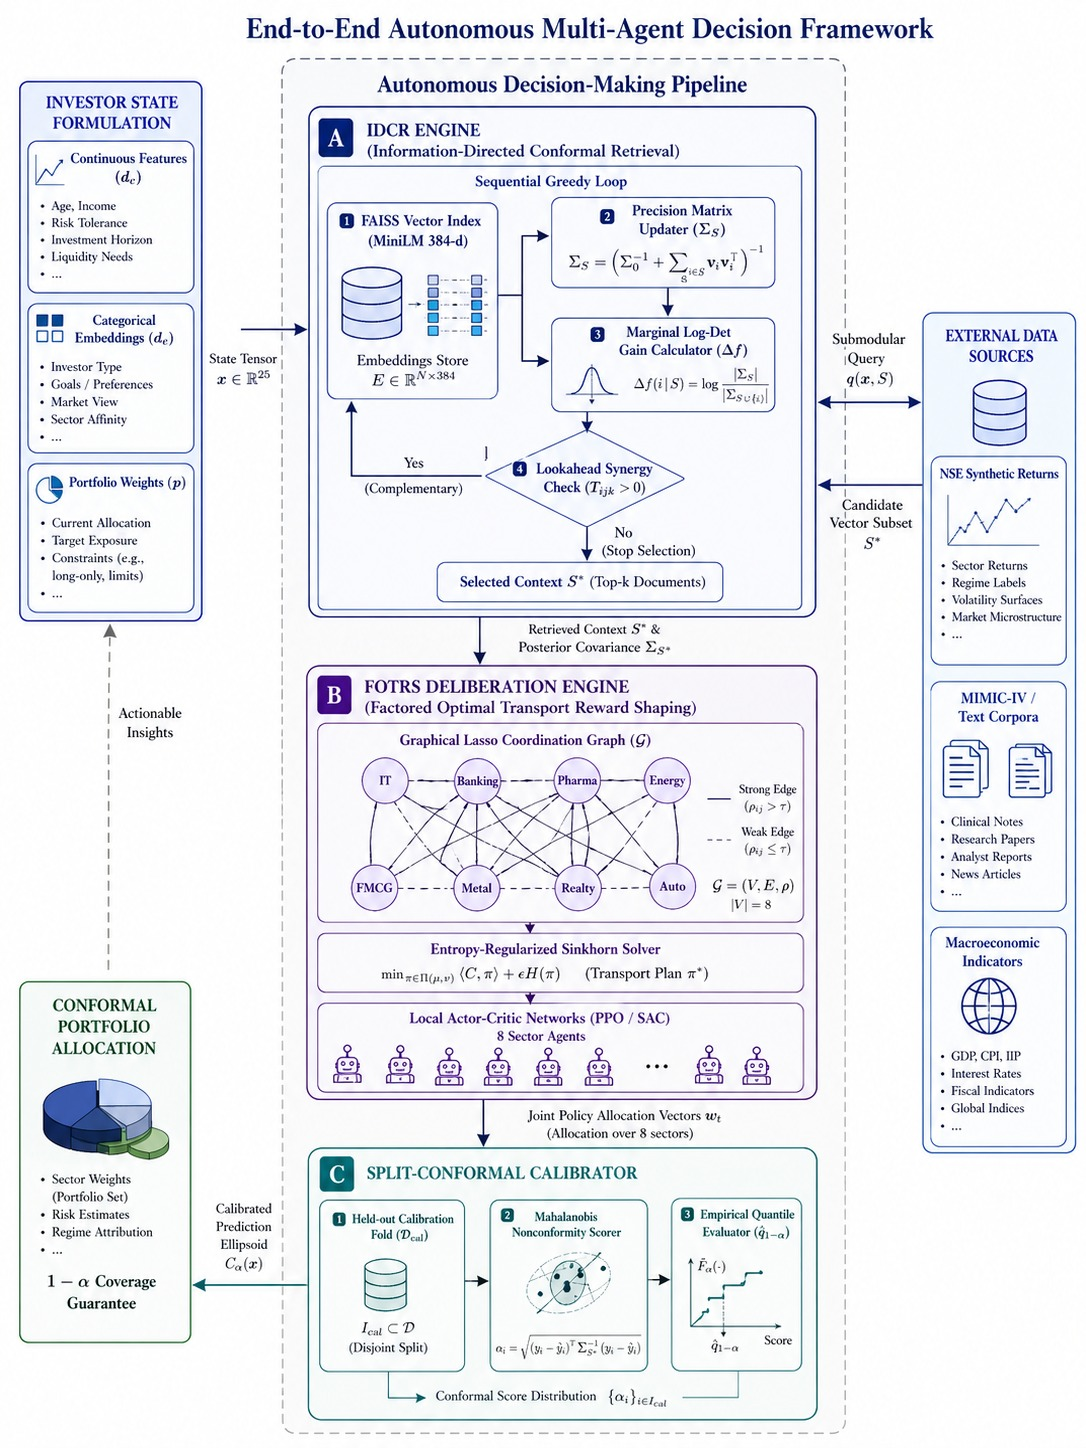
\includegraphics[width=0.95\textwidth]{figures/architecture.png}
    \caption{Architecture Diagram of the End-to-End Decision Framework}
    \label{fig:architecture}
\end{figure}

The architecture diagram demonstrates how the system processes information in discrete stages. The user inputs their financial profile and queries, which are processed by the query interpreter. The profile is sent to the IDCR module, which searches the domain-specific financial knowledge base for uncertainty-reducing information rather than textually similar documents. The relevant documents are passed to the FOTRS Multi-Agent Engine, where specialized agents deliberate based on the retrieved facts and their collaborative optimal transport policies. Finally, the system aggregates the outputs and calibrates them using the Conformal Predictor to construct a statistically guaranteed prediction set.

The underlying operational architecture seamlessly integrates several profoundly complimentary advanced computational components, including highly structured mathematically-directed information retrieval, inherently distribution-free uncertainty-aware statistical prediction, decentralized multi-agent algorithmic reasoning, and continuously dynamic adaptive learning mechanism protocols. These sophisticated mathematical components work synchronously and cooperatively together to unequivocally ensure that the system not only accurately produces highly optimized predictive recommendations but actively and rigorously evaluates the fundamental statistical reliability, exact variance boundaries, and geometric volume of those explicit recommendations, maintaining supreme systemic integrity even in the pervasive presence of highly incomplete, massively corrupted, or rapidly evolving real-time data information streams.

At the absolute mathematical core of the proposed conceptual framework lies the inviolable operating principle that external unstructured information retrieval and internal structured mathematical decision-making mathematically cannot and should not operate as entirely independent, disconnected, asynchronous processes. Instead, the advanced system iteratively and intelligently retrieves unstructured textual and numeric information explicitly based strictly upon its calculated metric contribution strictly toward minimizing the measurable statistical uncertainty variance inherent within the final optimal decision trajectory. This revolutionary mathematical approach enables the neural system to dynamically and gracefully prioritize exactly those documents that actively provide the highest level of mathematically meaningful, orthogonally independent evidence strictly for the bounding decision, proactively discarding documents that merely identically resemble the superficial input query textually through naive Euclidean semantic geometry.

To substantially further enhance the absolute, verifiable reliability of the overall mathematical decision process, the system natively incorporates advanced non-parametric conformal prediction mathematical techniques that inherently allow the architecture to explicitly produce strictly calibrated quantitative prediction bounding sets, entirely abandoning the hazardous practice of emitting single, overly-confident deterministic point outputs. These precise mathematical prediction sets provide a strictly theoretically grounded, distribution-free statistical representation of model uncertainty, actively allowing the neural system to explicitly communicate and guarantee the exact boundary range of all mathematically possible continuous outcomes that remain strictly consistent utilizing the totality of the currently available optimal evidence.

\section{Modules}

The architecture of the proposed system consists of several interconnected modules that collectively implement an autonomous decision-making pipeline. Each module performs a specific function within the overall reasoning process while interacting with other modules to refine the system's understanding of the problem.

\subsection{Investor Profiling Module}
The input to the system consists of a structured user profile card representing the investor's financial context. This profile includes attributes such as age, profession, investment horizon, current portfolio allocation, and risk tolerance. In the Information-Directed Conformal Retrieval formulation, this profile corresponds to the user state variable $x$, which conditions both the retrieval process and the portfolio recommendation generated by the system.

\medskip
\noindent\textbf{Formal State-Space Definition.}
The investor profile is encoded as a composite state vector $x \in \mathcal{X} \subseteq \mathbb{R}^{d_x}$, constructed by concatenating continuous and embedded categorical features. Specifically, the state vector decomposes as:
\[
x = \left[ x^{(\text{cont})} \;\|\; x^{(\text{cat})} \;\|\; x^{(\text{port})} \right] \in \mathbb{R}^{d_x},
\]
where each component captures a distinct aspect of the investor's context:
\begin{itemize}[leftmargin=2em]
  \item $x^{(\text{cont})} \in \mathbb{R}^{d_c}$ encodes the continuous numerical attributes: age (normalized to $[0,1]$), annual income (log-transformed), total investable assets, investment horizon in years, and monthly savings rate. These features are standardized to zero mean and unit variance using statistics computed on the training set.
  \item $x^{(\text{cat})} \in \mathbb{R}^{d_e}$ encodes the categorical attributes via learned dense embeddings: profession category (salaried, self-employed, retired), risk tolerance class (conservative, moderate, aggressive), investment experience level, and tax bracket. Each categorical variable is mapped through a trainable embedding layer $\text{Embed}_j : \{1, \ldots, C_j\} \to \mathbb{R}^{e_j}$, where $C_j$ is the cardinality of the $j$-th categorical variable and $e_j$ is the embedding dimension (typically $e_j = \min(50, \lceil C_j / 2 \rceil)$). The total categorical dimension is $d_e = \sum_j e_j$.
  \item $x^{(\text{port})} \in \mathbb{R}^{p}$ captures the investor's current portfolio allocation vector, where $p$ is the number of sectors. This provides the model with the baseline allocation from which rebalancing recommendations are computed.
\end{itemize}
\noindent The total state dimension is $d_x = d_c + d_e + p$. In the current implementation with $d_c = 5$ continuous features, $d_e = 12$ embedding dimensions across four categorical variables, and $p = 8$ sectors, the state vector has dimensionality $d_x = 25$.

\medskip
\noindent\textbf{Profile-Conditioned Prior Construction.}
The state vector $x$ directly conditions the prior distribution over portfolio allocations. The prior mean $\mu_0(x)$ and prior covariance $\Sigma_0(x)$ are computed by a neural network backbone $f_\theta : \mathbb{R}^{d_x} \to \mathbb{R}^p \times \mathbb{R}^{p \times p}$, trained on historical investor-outcome pairs. The architecture ensures that $\Sigma_0(x)$ is always positive definite by parameterizing the output as a Cholesky factor: $\Sigma_0(x) = L(x) L(x)^\top + \epsilon I_p$, where $L(x)$ is a lower-triangular matrix with positive diagonal entries (enforced via softplus activation) and $\epsilon > 0$ is a small regularization constant ensuring numerical stability.

The conditioning on $x$ is essential: an aggressive young investor with a long horizon will have a prior $\Sigma_0(x)$ with larger diagonal entries (higher acceptable uncertainty) and a mean $\mu_0(x)$ tilted toward equity-heavy allocations, whereas a conservative retiree will have a tighter prior concentrated near fixed-income allocations.

\medskip
\noindent\textbf{Query Processing Pipeline.}
The pipeline begins with the input stage, where a user query representing a real-world decision problem enters the system. The system first analyzes the query to determine the current state of the problem, identifying relevant variables and contextual information necessary for subsequent processing. In addition to the structured profile, the module accepts free-form natural language queries (e.g., ``Should I increase my pharma exposure given the upcoming budget session?''). These queries are processed through a domain-adapted sentence encoder to produce a query embedding $q \in \mathbb{R}^{d_q}$, which is appended to the state vector to form the augmented state $\tilde{x} = [x \| q]$. The augmented state $\tilde{x}$ is then passed to the IDCR module, where it conditions both the retrieval objective (which documents reduce uncertainty about this specific investor's optimal allocation) and the conformal calibration (which quantile threshold is appropriate for this investor's risk profile).

\subsection{Information-Directed Conformal Retrieval (IDCR) Module}
The limitations identified in earlier architectures highlighted three fundamental challenges that existing decision-making systems were unable to address effectively. First, traditional generative models frequently produced overly confident answers without any statistically reliable measure of uncertainty. In high-stakes domains such as quantitative finance or medical diagnostics, this inevitably leads to catastrophic errors, as the system cannot quantify what it does not know. Second, conventional reinforcement learning systems struggled immensely to recognize situations that differed significantly from the exact empirical data distributions they had previously encountered during their optimization phases, rendering them brittle in non-stationary environments. Third, and perhaps most critically for structural integrity, the entire upstream process of retrieving information from external knowledge bases was almost universally disjointed from the downstream mathematical requirements of the final decision-making process.

To address these profound limitations, the proposed framework introduces the Information-Directed Conformal Retrieval (IDCR) module. This advanced module mathematically integrates three interdependent concepts: distribution-free uncertainty-aware statistical prediction via split-conformal techniques, downstream decision-oriented informational retrieval, and diversity-aware spatial subset selection governed by monotone submodular optimization. Retrieval-augmented generation (RAG) traditionally ranks external documents utilizing purely geometric constructs traversing the embedding space, such as simple cosine similarity vector matching or BM25 lexical overlap functions. When information retrieval is driven solely by semantic similarity, the system implicitly ignores the fundamental mathematical effect of document selection on downstream predictive variance. Prioritizing documents merely because their terminology mimics the user's query can yield overconfident and needlessly imprecise predictions. This occurs largely because the retrieved documents often contain highly redundant information; they point in the exact same principal component directions that the reasoning model is already well-informed about. IDCR resolves this by explicitly modeling the document retrieval process as an active optimization objective aiming to minimize the precise geometric volume of downstream conformal prediction sets.

\subsubsection{Conformal Set Volume and the Log-Determinant Matrix Surrogate}

To operationalize this paradigm of uncertainty reduction mathematically, we rigorously formulate the decision estimation task by first establishing the formal notation, the problem definition, and the key modeling assumptions.

\medskip
\noindent\textbf{Notation and Problem Setup.} Let $x \in \mathcal{X} \subseteq \mathbb{R}^{d_x}$ be a high-dimensional query representation encoding the investor's comprehensive financial state. The state vector $x$ encompasses both continuous features (e.g., portfolio weights, account value, investment horizon in years) and categorical features (e.g., risk class, profession code) embedded into a continuous representation via learned embeddings. Let $\mathcal{D} = \{d_1, \ldots, d_N\}$ represent the unstructured document corpus containing $N$ financial text documents (market reports, regulatory filings, analyst notes, macroeconomic summaries). Each document $d \in \mathcal{D}$ is associated with a pre-computed dense embedding $\phi(d) \in \mathbb{R}^{p}$ obtained via a domain-adapted transformer encoder. The target variable $y^* \in \mathcal{Y} \subseteq \mathbb{R}^p$ represents the multidimensional decision output---in the portfolio allocation context, $y^* = (y^*_1, \ldots, y^*_p)$ is a continuous weight vector satisfying the simplex constraint $\sum_{j=1}^p y^*_j = 1$ and $y^*_j \geq 0$, where $p$ denotes the number of financial sectors under consideration.

\medskip
\noindent\textbf{Formal Problem Definition.}
The core retrieval problem can be stated as follows: given a query state $x$, a document corpus $\mathcal{D}$, a retrieval budget $k \ll N$, and a target miscoverage rate $\alpha \in (0,1)$, find the subset $S^* \subseteq \mathcal{D}$ with $|S^*| \leq k$ that minimizes the volume of the resulting conformal prediction set:
\[
S^* = \arg\min_{S \subseteq \mathcal{D},\; |S| \leq k} \text{Vol}\left(C_{\alpha}(x, S)\right).
\]
This optimization problem is computationally intractable in its exact form, since the number of candidate subsets is $\binom{N}{k}$, which grows combinatorially. For a corpus of $N = 10^6$ documents and a budget of $k = 10$, this amounts to approximately $2.63 \times 10^{53}$ candidate subsets. The key insight of IDCR is that this problem admits an efficient approximate solution via submodular optimization, as we formalize below.

\medskip
\noindent\textbf{Modeling Assumptions.}
The derivation of the tractable surrogate objective relies on two key assumptions, which we state explicitly and justify:

\begin{enumerate}[leftmargin=2em]
  \item \textbf{Gaussian Prior (Tractability Assumption):} Before any external documents are retrieved from the corpus, the target variable follows a query-conditioned Gaussian prior:
  \[
  y^* \mid x \sim \mathcal{N}(\mu_0(x),\; \Sigma_0(x)).
  \]
  The mean $\mu_0(x) \in \mathbb{R}^p$ represents the model's initial best estimate of the optimal allocation (e.g., an equal-weight or market-cap-weighted baseline), and the covariance matrix $\Sigma_0(x) \in \mathbb{R}^{p \times p}$ captures the full uncertainty structure, including cross-sector correlations.

  \textit{Justification:} The Gaussian assumption is motivated by three considerations. First, it yields a closed-form posterior under linear-Gaussian updates, enabling tractable computation of the gain function $g(S)$. Second, the Central Limit Theorem provides a theoretical basis: portfolio returns (being weighted sums of individual asset returns) are approximately Gaussian for well-diversified portfolios. Third, and most importantly, the conformal prediction framework provides distribution-free coverage guarantees regardless of the true data distribution---the Gaussian assumption affects only the \emph{efficiency} (tightness) of the prediction sets, not their \emph{validity} (coverage guarantee). Even if the true distribution is non-Gaussian, the conformal coverage bound $\mathbb{P}(y^* \in C_{\alpha}) \geq 1 - \alpha$ still holds.

  \item \textbf{Conditional Independence of Document Contributions:} Each document $d \in S$ contributes an independent precision increment $\Lambda_d(x) \succeq 0$ to the posterior, conditioned on the query $x$:
  \[
  \Sigma(x, S)^{-1} = \Sigma_0(x)^{-1} + \sum_{d \in S} \Lambda_d(x).
  \]
  \textit{Justification:} This additive precision structure is standard in Bayesian sensor fusion and experimental design. It models documents as independent ``informational sensors'': each document provides a noisy ``observation'' of the target $y^*$, and the precision of each observation is encoded in $\Lambda_d(x)$. The conditional independence assumption is reasonable when documents are drawn from diverse sources (different analysts, different time periods, different sectors), ensuring that their informational content does not exhibit strong positive correlation. When documents are indeed redundant, the submodularity property (Theorem~1) automatically handles this by assigning diminishing marginal returns to redundant additions.
\end{enumerate}

\medskip
\noindent\textbf{Retrieval Policy and Calibration Set.}
An algorithmic retrieval policy $\pi$ sequentially selects a specific subset of documents denoted as $S \subset \mathcal{D}$, strictly limited to an operational budget size $k \ll N$ to maintain system latency. The budget $k$ introduces a fundamental trade-off: larger $k$ permits more uncertainty reduction (smaller prediction sets) at the cost of increased retrieval latency and computational overhead. In our implementation, setting $k = 10$ yields a favorable balance with per-query retrieval latency under 17 ms.

Once the knowledge context $S$ is retrieved, a split-conformal predictor, calibrated on a completely disjoint held-out dataset $\mathcal{D}_{\text{cal}} = \{(x_i, S_i, y_i)\}_{i=1}^m$, processes the inputs to produce a statistically guaranteed prediction set. The split-conformal methodology requires that the calibration set $\mathcal{D}_{\text{cal}}$ be strictly disjoint from both the training set (used to learn the model parameters $\mu(\cdot)$ and $\Sigma(\cdot)$) and the document corpus $\mathcal{D}$ (from which documents are retrieved). This separation is essential: if calibration data were used during training, the nonconformity scores would be biased downward, leading to under-coverage. In our setting, we reserve $m = 500$ calibration examples, providing a quantile resolution of $1/501 \approx 0.2\%$.

In a robust probabilistic setting, before any external documents are retrieved from the corpus, the target variable follows the query-conditioned prior distribution $y^* \mid x \sim \mathcal{N}(\mu_0, \Sigma_0(x))$. Here, the initial covariance matrix $\Sigma_0(x)$ comprehensively encapsulates the baseline epistemic and aleatoric uncertainty regarding the optimal allocation prior to observing any external supporting evidence. Assuming the nonconformity measure utilizes the precision-weighted Mahalanobis distance metric, the resulting output decision set is defined as:
\begin{equation} \label{eq:conformal_set}
C_{\alpha}(x, S) = \left\{ y \in \mathbb{R}^p : s(x, S, y) \leq \hat{q}_{1-\alpha}(S) \right\}
\end{equation}

\medskip
\noindent This equation defines the \emph{conformal prediction set}, which is the central output object of the IDCR framework. Rather than producing a single point prediction $\hat{y}$, the system outputs an entire \emph{set} of plausible decision vectors. The components of this equation are as follows:

\begin{itemize}[leftmargin=2em]
  \item $C_{\alpha}(x, S)$ denotes the conformal prediction set, parameterized by the miscoverage rate $\alpha \in (0,1)$, the user query state $x$, and the retrieved document subset $S$. The set collects all candidate decision vectors $y$ that are deemed ``consistent'' with the observed evidence at the target confidence level $1 - \alpha$.
  \item $y \in \mathbb{R}^p$ represents a candidate decision output. In the financial application, $y$ is a $p$-dimensional continuous portfolio allocation weight vector, where each component $y_j$ represents the fractional capital allocation to the $j$-th market sector.
  \item $s(x, S, y)$ is the \emph{nonconformity score function}, which measures how ``unusual'' or ``non-conforming'' a candidate output $y$ is relative to the model's learned conditional distribution given input $x$ and context $S$. A smaller score indicates that $y$ is more consistent with the historical calibration data.
  \item $\hat{q}_{1-\alpha}(S)$ is the \emph{empirical quantile threshold}, computed as the $\lceil(1-\alpha)(m+1)\rceil / m$ quantile of the nonconformity scores $\{s(x_i, S_i, y_i)\}_{i=1}^m$ evaluated on the held-out calibration set $\mathcal{D}_{\text{cal}}$. This threshold acts as a ``gate'': any candidate $y$ whose nonconformity score does not exceed $\hat{q}_{1-\alpha}$ is included in the prediction set.
\end{itemize}

\noindent The geometric interpretation of this equation is fundamental: the set $C_{\alpha}(x, S)$ is the \emph{sub-level set} of the nonconformity score function at height $\hat{q}_{1-\alpha}$. Under the Mahalanobis scoring function defined below, this sub-level set takes the shape of a $p$-dimensional ellipsoid in the decision space $\mathbb{R}^p$. The volume of this ellipsoid directly quantifies the system's residual uncertainty: a smaller ellipsoid corresponds to a more precise and actionable recommendation.

\medskip
\noindent The Mahalanobis nonconformity score function evaluates the spatial distance from the conditional mean $\mu(x,S)$ scaled proportionally by the inverse matrix of the posterior covariance:
\begin{equation} \label{eq:mahalanobis_score}
s(x, S, y) = (y - \mu(x,S))^\top \Sigma(x, S)^{-1} (y - \mu(x,S))
\end{equation}

\medskip
\noindent This equation defines the specific nonconformity measure used by the IDCR framework. The Mahalanobis distance is a generalization of the standard Euclidean distance that accounts for the correlation structure between dimensions:

\begin{itemize}[leftmargin=2em]
  \item $(y - \mu(x,S))$ is the \emph{residual vector}, representing the deviation of the candidate output $y$ from the model's conditional mean prediction $\mu(x,S)$. The mean $\mu(x,S)$ is the model's best single-point estimate of the optimal decision, conditioned on the user state $x$ and the retrieved documents $S$.
  \item $\Sigma(x, S)^{-1}$ is the \emph{precision matrix} (inverse covariance matrix) of the posterior predictive distribution. This matrix encodes the model's uncertainty structure: the $(j,k)$-th entry of $\Sigma(x,S)$ captures the covariance between the $j$-th and $k$-th components of the decision vector. By using the inverse $\Sigma^{-1}$, the score naturally downweights deviations along high-variance directions (where the model is already uncertain) and amplifies deviations along low-variance directions (where the model is confident).
  \item The quadratic form $v^\top M v$ for a positive-definite matrix $M$ produces a non-negative scalar. When $M = I$ (the identity matrix), this reduces to the ordinary squared Euclidean distance $\|y - \mu\|^2$. When $M = \Sigma^{-1}$, the distance is ``stretched'' along the principal axes of the covariance ellipsoid, producing the Mahalanobis distance.
\end{itemize}

\noindent Under the Gaussian modeling assumption $y^* \mid x, S \sim \mathcal{N}(\mu(x,S), \Sigma(x,S))$, the score $s(x,S,y^*)$ follows a chi-squared distribution with $p$ degrees of freedom, i.e., $s(x,S,y^*) \sim \chi^2_p$. This distributional characterization provides a useful sanity check: on the calibration set, the scores should empirically approximate a $\chi^2_p$ distribution.

\medskip
\noindent The threshold scalar $\hat{q}_{1-\alpha}(S)$ represents the empirically calculated $\lceil(1-\alpha)(|\mathcal{D}_{\text{cal}}| + 1)\rceil / |\mathcal{D}_{\text{cal}}|$ quantile derived entirely over the historically observed validation nonconformity scores present within the independent calibration set. Concretely, given the calibration scores $s_1 \leq s_2 \leq \cdots \leq s_m$ sorted in non-decreasing order, the threshold is $\hat{q}_{1-\alpha} = s_{(j)}$ where $j = \lceil (1-\alpha)(m+1) \rceil$. If $j > m$, we set $\hat{q}_{1-\alpha} = +\infty$, yielding a trivial prediction set $C_{\alpha} = \mathbb{R}^p$.

The paramount mathematical guarantee provided by classical split-conformal prediction theory precisely ensures that as long as the calibration data points $(x,y)$ are statistically exchangeable, and provided that the automated retrieval policy $\pi$ operates strictly on the observable features $x$ and the unsupervised document representations without inappropriately observing the eventual target value $y^*$, then an absolute distribution-free marginal statistical coverage rigidly and universally holds true under any potential data generating process:
\begin{equation} \label{eq:coverage_guarantee}
\mathbb{P}\left(y^* \in C_{\alpha}(x, S^\pi)\right) \geq 1 - \alpha
\end{equation}

\medskip
\noindent This is the \emph{finite-sample coverage guarantee}, the most powerful theoretical property of conformal prediction. It states that the probability that the true (unknown) optimal decision $y^*$ lies inside the prediction set $C_{\alpha}$ is at least $1 - \alpha$, regardless of the true data-generating distribution. The components are:

\begin{itemize}[leftmargin=2em]
  \item $\mathbb{P}(\cdot)$ denotes the probability over the randomness in \emph{both} the calibration data and the new test point $(x, y^*)$.
  \item $y^*$ is the unknown true optimal decision for the new test query.
  \item $S^\pi$ emphasizes that the retrieved document subset was selected by the policy $\pi$ without observing $y^*$.
  \item $1 - \alpha$ is the \emph{target coverage level}. For example, setting $\alpha = 0.10$ guarantees that $y^*$ is captured at least $90\%$ of the time.
\end{itemize}

\noindent Crucially, this guarantee is \emph{distribution-free}: it holds for any joint distribution of $(x, y^*)$, not just Gaussian or any other parametric family. The only requirement is \emph{exchangeability} of the calibration and test data, a strictly weaker condition than the standard i.i.d.\ assumption.

\begin{proof}[\textbf{Proof.}]
Let the calibration dataset be $\mathcal{D}_{\text{cal}} = \{(x_1, S_1, y_1), \ldots, (x_m, S_m, y_m)\}$ and let $(x_{m+1}, S_{m+1}, y_{m+1})$ denote the new test point. By assumption, these $m+1$ data points are exchangeable, meaning their joint distribution is invariant under any permutation of indices.

Define the nonconformity scores:
\[
V_i = s(x_i, S_i, y_i), \quad i = 1, \ldots, m+1.
\]
Since the score function $s$ is a fixed (measurable) function and the data points are exchangeable, the scores $V_1, V_2, \ldots, V_{m+1}$ are themselves exchangeable random variables.

By the fundamental property of exchangeable random variables, for any fixed realization, every permutation of the indices is equally likely. Therefore, the rank of $V_{m+1}$ among $\{V_1, \ldots, V_{m+1}\}$ is uniformly distributed over $\{1, 2, \ldots, m+1\}$:
\[
\mathbb{P}\left(\text{rank}(V_{m+1}) = j\right) = \frac{1}{m+1}, \quad j = 1, \ldots, m+1.
\]

Now, define the empirical quantile threshold as:
\[
\hat{q}_{1-\alpha} = \inf\left\{q : \frac{|\{i \in \{1,\ldots,m\} : V_i \leq q\}|}{m} \geq \frac{\lceil(1-\alpha)(m+1)\rceil}{m}\right\}.
\]
This is equivalently the $\lceil(1-\alpha)(m+1)\rceil$-th smallest value among $V_1, \ldots, V_m$. Let $p = \lceil(1-\alpha)(m+1)\rceil$.

The test point is covered, i.e., $y_{m+1} \in C_{\alpha}(x_{m+1}, S_{m+1})$, if and only if:
\[
V_{m+1} \leq \hat{q}_{1-\alpha}.
\]
This event occurs precisely when $V_{m+1}$ is at most the $p$-th smallest among all $m+1$ scores, i.e., when $\text{rank}(V_{m+1}) \leq p$. By the uniform rank distribution:
\[
\mathbb{P}\left(V_{m+1} \leq \hat{q}_{1-\alpha}\right) \geq \frac{p}{m+1} = \frac{\lceil(1-\alpha)(m+1)\rceil}{m+1} \geq 1 - \alpha,
\]
where the final inequality follows from the ceiling function: $\lceil(1-\alpha)(m+1)\rceil \geq (1-\alpha)(m+1)$, so $\frac{\lceil(1-\alpha)(m+1)\rceil}{m+1} \geq 1-\alpha$.

This completes the proof. Note that no assumption on the distribution of $(x,y)$ was needed beyond exchangeability. The guarantee is also \emph{finite-sample}: it holds exactly for any calibration set size $m$, not just asymptotically.
\end{proof}

By actively utilizing the precision-weighted Mahalanobis scoring function under the specified Gaussian modeling framework, the absolute physical geometry enveloping the conformal prediction set $C_{\alpha}(x, S)$ naturally contours into a highly complex $p$-dimensional multivariate ellipsoid existing formally within the continuous decision space parameters. If the primary computational directive of the underlying retrieval mechanism insists upon producing the mathematically sharpest and highly explicit actionable decision bounds, the fundamental optimization objective must absolutely logically structure itself to computationally minimize the exact contiguous multidimensional spatial hyper-volume defined enclosing this specific prediction ellipsoid. Computing the absolute volumetric geometry representing an entirely arbitrary high-dimensional ellipsoid governed structurally via an integrated covariance matrix $\Sigma$ is expressed exactly mathematically, and calculating the corresponding natural logarithmic transformation mapping its bounding topological volume explicitly separates dynamically into three unequivocally distinct analytical components:
\begin{equation} \label{eq:log_volume}
\log \text{Vol}(C_{\alpha}(x, S)) = \log c_p + \frac{1}{2} \log \det \Sigma(x, S) + \frac{p}{2} \log \hat{q}_{1-\alpha}(S)
\end{equation}
where $c_p$ denotes the volume of the $p$-dimensional unit ball, given by $c_p = \pi^{p/2} / \Gamma(p/2 + 1)$.

\medskip
\noindent This equation decomposes the logarithmic volume of the conformal prediction ellipsoid into three interpretable terms. The derivation proceeds from first principles.

Recall that the conformal prediction set $C_{\alpha}(x, S) = \{y : (y - \mu)^\top \Sigma^{-1} (y - \mu) \leq \hat{q}_{1-\alpha}\}$ is a $p$-dimensional ellipsoid. The standard formula for the volume of such an ellipsoid is obtained through a change of variables. Let $z = \Sigma^{-1/2}(y - \mu)$, so that $y = \Sigma^{1/2} z + \mu$. The Jacobian of this transformation is $|\det(\Sigma^{1/2})| = (\det \Sigma)^{1/2}$. Under this substitution, the set becomes $\{z \in \mathbb{R}^p : \|z\|^2 \leq \hat{q}_{1-\alpha}\}$, which is a ball of radius $r = \sqrt{\hat{q}_{1-\alpha}}$. Therefore:
\[
\text{Vol}(C_{\alpha}) = \text{Vol}\left(B_p\left(\sqrt{\hat{q}_{1-\alpha}}\right)\right) \cdot (\det \Sigma)^{1/2}
= c_p \cdot \left(\hat{q}_{1-\alpha}\right)^{p/2} \cdot (\det \Sigma)^{1/2},
\]
where $B_p(r)$ denotes the $p$-ball of radius $r$ and $c_p = \pi^{p/2}/\Gamma(p/2+1)$ is the volume of the $p$-dimensional unit ball. Taking logarithms yields exactly:
\[
\log \text{Vol}(C_{\alpha}) = \underbrace{\log c_p}_{\text{dimension-dependent constant}} + \underbrace{\frac{1}{2} \log \det \Sigma(x,S)}_{\text{covariance contribution}} + \underbrace{\frac{p}{2} \log \hat{q}_{1-\alpha}(S)}_{\text{quantile contribution}}.
\]

The three terms have distinct roles:
\begin{itemize}[leftmargin=2em]
  \item $\log c_p$ is a universal constant depending only on the dimensionality $p$ of the decision space. For $p = 8$ sectors, $c_8 = \pi^4/24 \approx 4.06$. This term is invariant to the retrieval policy and can be ignored during optimization.
  \item $\frac{1}{2} \log \det \Sigma(x,S)$ captures the ``spread'' of the posterior covariance. As more informative documents are retrieved, $\Sigma(x,S)$ shrinks, its determinant decreases, and this term becomes more negative, reducing the total volume.
  \item $\frac{p}{2} \log \hat{q}_{1-\alpha}(S)$ captures the contribution of the empirical quantile threshold. For a fixed coverage level $1-\alpha$ and sufficiently large calibration set, this term exhibits negligible variation across different retrieval subsets $S$ of the same size $k$.
\end{itemize}

A critical engineering observation is that the quantile term $\hat{q}_{1-\alpha}(S)$ exhibits approximately zero variance across different subsets of size $k$, provided the calibration dataset possesses sufficient cardinality. This is because the quantile is computed over the fixed calibration set and the retrieval policy does not modify the calibration data. Consequently, the log-determinant of the posterior covariance matrix isolates itself as the single dominant variable, establishing an exact surrogate proxy for volume reduction:
\begin{equation} \label{eq:gain_function}
g(S) = \log \det \Sigma_0(x) - \log \det \Sigma(x, S)
\end{equation}

\medskip
\noindent The function $g(S)$ measures the \emph{information gain} achieved by retrieving the document subset $S$. It is the difference between the log-determinant of the prior covariance (before retrieval) and the posterior covariance (after retrieval):
\begin{itemize}[leftmargin=2em]
  \item $\log \det \Sigma_0(x)$ is the log-volume contribution of the prior uncertainty (before any documents are retrieved). This is a constant with respect to $S$.
  \item $\log \det \Sigma(x,S)$ is the log-volume contribution of the posterior uncertainty after incorporating the information from subset $S$.
  \item Since $\Sigma(x,S) \preceq \Sigma_0(x)$ (adding information can only reduce or maintain the covariance), we have $\det \Sigma(x,S) \leq \det \Sigma_0(x)$, which guarantees $g(S) \geq 0$.
  \item Maximizing $g(S)$ is equivalent to minimizing $\log \det \Sigma(x,S)$, which in turn minimizes the volume of the conformal ellipsoid (up to the constant terms identified above).
\end{itemize}

\noindent This function has a deep connection to information theory. Under the Gaussian model, $g(S)$ equals twice the mutual information $I(y^*; \{\phi(d) : d \in S\} \mid x)$ between the target variable and the document embeddings, conditioned on the query. Thus, maximizing $g(S)$ is equivalent to maximizing the mutual information between the retrieved evidence and the decision target.

\medskip
\noindent Using standard foundational properties of linear algebra wherein the determinant of a matrix is inversely proportional to the determinant of its inverse mathematical counterpart ($\det \Sigma = \det \Omega^{-1}$, where the precision matrix is defined as $\Omega = \Sigma^{-1}$), the core optimization objective $g(S)$ is analytically equivalent to:
\begin{equation} \label{eq:idcr_gain}
g(S) = \log \det\left(\Sigma_0(x)^{-1} + \sum_{d \in S} \Lambda_d(x)\right) - \log \det \Sigma_0(x)^{-1}
\end{equation}

\medskip
\noindent This equation re-expresses the gain function $g(S)$ entirely in terms of \emph{precision matrices} rather than covariance matrices. The derivation is as follows.

Starting from $g(S) = \log \det \Sigma_0 - \log \det \Sigma(x,S)$, we use the identity $\det(A^{-1}) = 1/\det(A)$, which implies $\log \det(A^{-1}) = -\log \det(A)$. Therefore:
\begin{align*}
g(S) &= \log \det \Sigma_0 - \log \det \Sigma(x,S) \\
&= -\log \det \Sigma_0^{-1} + \log \det \Sigma(x,S)^{-1} \\
&= \log \det \Sigma(x,S)^{-1} - \log \det \Sigma_0^{-1}.
\end{align*}

Substituting the Bayesian precision update rule $\Sigma(x,S)^{-1} = \Sigma_0^{-1} + \sum_{d \in S} \Lambda_d(x)$ (derived below), we obtain:
\[
g(S) = \log \det\left(\Sigma_0^{-1} + \sum_{d \in S} \Lambda_d(x)\right) - \log \det \Sigma_0^{-1}.
\]

The key components of this expression are:
\begin{itemize}[leftmargin=2em]
  \item $\Sigma_0(x)^{-1}$ is the \emph{prior precision matrix}, representing the model's initial level of certainty before observing any documents.
  \item Each $\Lambda_d(x) \succeq 0$ is the \emph{precision contribution matrix} of document $d$. The notation $\Lambda_d(x) \succeq 0$ means that $\Lambda_d(x)$ is positive-semidefinite, ensuring that adding document $d$ can only increase precision (reduce uncertainty) or leave it unchanged.
  \item The sum $\sum_{d \in S} \Lambda_d(x)$ reflects the \emph{additive aggregation} of precision contributions. This additivity is a consequence of the independence assumption: conditioned on the query $x$, the informational contributions of different documents are modeled as independent precision increments.
\end{itemize}

In practice, the precision matrix $\Lambda_d(x)$ for each document $d$ is computed by passing the document embedding $\phi(d) \in \mathbb{R}^p$ through a learned precision mapping network $h_\theta(\cdot)$ that outputs a rank-one or low-rank positive-semidefinite matrix: $\Lambda_d(x) = \sigma^{-2}(x) \cdot \phi(d) \phi(d)^\top$, where $\sigma^{-2}(x)$ is a query-dependent scaling factor.

\medskip
\noindent Each individual unstructured text document $d$ mathematically maps to a continuous positive-semidefinite predictive precision matrix $\Lambda_d(x) \succeq 0$, quantitatively formalizing how significantly the inclusion of document $d$ collapses the variance of the model's hypotheses regarding the optimal allocation target $y^*$. Instead of extracting documents based on shallow keyword matching or geometric cosine approximations, IDCR elegantly frames the text retrieval problem as a Bayesian precision aggregation update mechanism:
\begin{equation} \label{eq:bayesian_update}
\Sigma(x, S)^{-1} = \Sigma_0(x)^{-1} + \sum_{d \in S} \Lambda_d(x)
\end{equation}

\medskip
\noindent This equation is the \emph{Bayesian precision update rule}, which is the mathematical engine underlying the entire IDCR framework. It states that the posterior precision matrix (after observing documents $S$) equals the prior precision matrix plus the sum of all individual document precision contributions.

This rule arises naturally from Bayesian linear regression. Consider the model:
\[
y^* = \mu_0 + \sum_{d \in S} \Lambda_d^{1/2}(x) \cdot \epsilon_d + \eta, \quad \eta \sim \mathcal{N}(0, \Sigma_0(x)),
\]
where each document $d$ provides an independent observation $\phi(d)$ of the target with precision $\Lambda_d(x)$. By the standard conjugate Gaussian update, the posterior distribution is:
\[
y^* \mid x, S \sim \mathcal{N}\left(\mu(x,S),\; \left(\Sigma_0(x)^{-1} + \sum_{d \in S} \Lambda_d(x)\right)^{-1}\right),
\]
which immediately gives the precision update: $\Sigma(x,S)^{-1} = \Sigma_0(x)^{-1} + \sum_{d \in S} \Lambda_d(x)$.

The key properties of this update rule are:
\begin{itemize}[leftmargin=2em]
  \item \textbf{Monotonicity:} Since each $\Lambda_d(x) \succeq 0$, adding a document to $S$ can only increase the precision (in the positive-semidefinite ordering), i.e., $\Sigma(x, S \cup \{d\})^{-1} \succeq \Sigma(x,S)^{-1}$.
  \item \textbf{Commutativity:} The order in which documents are added does not affect the final posterior. This is a direct consequence of the additivity of the precision contributions.
  \item \textbf{Diminishing returns:} The marginal reduction in uncertainty from adding a document $d$ is always smaller when added to a larger set (this is the submodularity property, formalized in Theorem~1).
  \item \textbf{Connection to Fisher Information:} Each $\Lambda_d(x)$ can be interpreted as the Fisher information matrix contributed by document $d$. The total Fisher information is the sum of individual contributions, which is the foundational principle underlying the additivity of precision in this update.
\end{itemize}

\subsubsection{Theoretical Formalization of Submodularity and Greedy Combinatorial Guarantees}

When attempting to algorithmically select the optimal discrete configuration of multiple interacting documents from an exceedingly massive corpus to absolutely maximize system decision support, exhaustively searching all possible permutations is notoriously intractable due to the vicious combinatorial explosion scaling as $\binom{N}{k}$. However, calculating the optimal subset efficiently becomes profoundly attainable because information inherently exhibits diminishing marginal returns when evaluated through the lens of variance reduction. The proposed mathematical framework formalizes this pivotal intuition through the structural algebraic property known as submodularity.

\textbf{Theorem 1 (Monotone Submodularity of the IDCR Surrogate Objective).} Let the precision contribution $\Lambda_d(x)$ be unconditionally positive-semidefinite matrix operators. Then, the mathematical gain function $g(S)$ established in Equation \ref{eq:idcr_gain} fundamentally satisfies the conditions of being a normalized, monotone, and strictly submodular set function over any discrete subset $S \subseteq \mathcal{D}$.

This theorem implies that the marginal utility of retrieving an additional document diminishes as more documents are gathered. By exploiting this property, the document selection process can be efficiently approximated using greedy optimization strategies.

\begin{proof}[\textbf{Proof.}]
We must verify three properties: normalization, monotonicity, and submodularity.

\medskip
\noindent\textit{Part 1: Normalization.}
We must show that $g(\emptyset) = 0$. When $S = \emptyset$, no documents are retrieved, so $\Sigma(x, \emptyset) = \Sigma_0(x)$ (the prior covariance is unchanged). Substituting into the definition:
\[
g(\emptyset) = \log \det \Sigma_0(x) - \log \det \Sigma_0(x) = 0. \qquad \checkmark
\]

\medskip
\noindent\textit{Part 2: Monotonicity.}
We must show that for any $S \subseteq T \subseteq \mathcal{D}$, we have $g(S) \leq g(T)$.

Define the precision matrices $\Omega_S = \Sigma_0^{-1} + \sum_{d \in S} \Lambda_d$ and $\Omega_T = \Sigma_0^{-1} + \sum_{d \in T} \Lambda_d$. Since $S \subseteq T$ and each $\Lambda_d \succeq 0$, we have:
\[
\Omega_T = \Omega_S + \sum_{d \in T \setminus S} \Lambda_d \succeq \Omega_S \succ 0,
\]
where the inequality is in the positive-semidefinite (L\"owner) ordering. A fundamental property of the determinant on the cone of positive-definite matrices states that if $A \succeq B \succ 0$, then $\det A \geq \det B$ (with equality if and only if $A = B$). Therefore:
\[
\det \Omega_T \geq \det \Omega_S \implies \log \det \Omega_T \geq \log \det \Omega_S.
\]
Since $g(S) = \log \det \Omega_S - \log \det \Sigma_0^{-1}$, we conclude $g(T) \geq g(S)$. $\checkmark$

\medskip
\noindent\textit{Part 3: Submodularity.}
We must show that for any $A \subseteq B \subseteq \mathcal{D}$ and any element $d \notin B$:
\[
\Delta_d(A) \triangleq g(A \cup \{d\}) - g(A) \geq g(B \cup \{d\}) - g(B) \triangleq \Delta_d(B).
\]
This is the \emph{diminishing marginal returns} property: adding document $d$ to a smaller set $A$ yields at least as much gain as adding it to a larger set $B \supseteq A$.

Define $\Omega_A = \Sigma_0^{-1} + \sum_{d' \in A} \Lambda_{d'}$ and $\Omega_B = \Sigma_0^{-1} + \sum_{d' \in B} \Lambda_{d'}$. Then:
\begin{align*}
\Delta_d(A) &= \log \det(\Omega_A + \Lambda_d) - \log \det \Omega_A \\
&= \log \det\left(\Omega_A^{-1/2}(\Omega_A + \Lambda_d)\Omega_A^{-1/2}\right) && \text{(similarity transform)} \\
&= \log \det\left(I + \Omega_A^{-1/2} \Lambda_d \, \Omega_A^{-1/2}\right).
\end{align*}

Similarly, $\Delta_d(B) = \log \det\left(I + \Omega_B^{-1/2} \Lambda_d \, \Omega_B^{-1/2}\right)$.

Since $A \subseteq B$, we have $\Omega_B \succeq \Omega_A \succ 0$, which implies $\Omega_B^{-1} \preceq \Omega_A^{-1}$ (matrix inverse reverses the ordering). Consequently:
\[
\Omega_B^{-1/2} \Lambda_d \, \Omega_B^{-1/2} \preceq \Omega_A^{-1/2} \Lambda_d \, \Omega_A^{-1/2}.
\]

To see why this inequality holds, note that for any positive-definite $M_1 \preceq M_2$ and positive-semidefinite $\Lambda$, the congruence $M_1^{1/2} \Lambda M_1^{1/2} \preceq M_2^{1/2} \Lambda M_2^{1/2}$ follows from the operator monotonicity of the square root. Since $\Omega_A^{-1} \succeq \Omega_B^{-1}$, taking $M_1 = \Omega_B^{-1}$ and $M_2 = \Omega_A^{-1}$, we obtain the desired PSD ordering.

Now, the function $X \mapsto \log \det(I + X)$ is monotone non-decreasing on the cone of positive-semidefinite matrices: if $0 \preceq X_1 \preceq X_2$, then $I + X_1 \preceq I + X_2$, and therefore $\det(I + X_1) \leq \det(I + X_2)$, giving $\log \det(I + X_1) \leq \log \det(I + X_2)$.

Applying this with $X_1 = \Omega_B^{-1/2} \Lambda_d \Omega_B^{-1/2}$ and $X_2 = \Omega_A^{-1/2} \Lambda_d \Omega_A^{-1/2}$:
\[
\Delta_d(B) = \log \det(I + X_1) \leq \log \det(I + X_2) = \Delta_d(A).
\]
This establishes the submodularity of $g(S)$. $\checkmark$

\medskip
Combining all three parts, $g(S)$ is a normalized, monotone, submodular set function. This completes the proof.
\end{proof}

\textbf{Corollary 1 (Greedy guarantee).} The sequential greedy policy satisfies:
\begin{equation} \label{eq:greedy_bound}
g(S_{\text{greedy}}) \geq \left(1 - \frac{1}{e}\right) g(S^*)
\end{equation}
where $S^*$ is the optimal configuration. This ensures that the greedy selection achieves at least $\approx 63\%$ of the optimal uncertainty reduction, while operating in $\mathcal{O}(kN)$ time per query compared to the intractable exhaustive search.

\begin{proof}[\textbf{Proof.}]
This result follows from the classical theorem of Nemhauser, Wolsey, and Fisher (1978) applied to the monotone submodular function $g(S)$ established in Theorem~1, subject to the cardinality constraint $|S| \leq k$.

The greedy algorithm constructs the set $S_{\text{greedy}} = \{d_1^*, d_2^*, \ldots, d_k^*\}$ by iteratively selecting the element with the largest marginal gain:
\[
d_t^* = \arg\max_{d \in \mathcal{D} \setminus S_{t-1}} \Delta_d(S_{t-1}) = \arg\max_{d \in \mathcal{D} \setminus S_{t-1}} \left[g(S_{t-1} \cup \{d\}) - g(S_{t-1})\right],
\]
where $S_0 = \emptyset$ and $S_t = S_{t-1} \cup \{d_t^*\}$.

Let $S^* = \{e_1, e_2, \ldots, e_k\}$ be any optimal subset of size $k$. We proceed by induction on the greedy steps.

\medskip
\noindent\textit{Step 1: Bounding the gap at each iteration.}
At iteration $t$, by submodularity and the greedy selection rule:
\begin{align*}
g(S^*) &\leq g(S_t \cup S^*) && \text{(monotonicity)} \\
&\leq g(S_t) + \sum_{j=1}^{k} \Delta_{e_j}(S_t) && \text{(submodularity applied iteratively)} \\
&\leq g(S_t) + k \cdot \Delta_{d_{t+1}^*}(S_t) && \text{(greedy chose the best single element)} \\
&= g(S_t) + k \cdot [g(S_{t+1}) - g(S_t)].
\end{align*}

The second inequality uses the telescoping property of submodularity: for any set $T = \{e_1, \ldots, e_k\}$ and any set $A$:
\[
g(A \cup T) - g(A) \leq \sum_{j=1}^{k} \Delta_{e_j}(A),
\]
which holds because submodularity implies $\Delta_{e_j}(A \cup \{e_1, \ldots, e_{j-1}\}) \leq \Delta_{e_j}(A)$.

The third inequality follows because the greedy algorithm selects $d_{t+1}^* = \arg\max_d \Delta_d(S_t)$, so $\Delta_{d_{t+1}^*}(S_t) \geq \Delta_{e_j}(S_t)$ for every $j$.

\medskip
\noindent\textit{Step 2: Defining the gap sequence.}
Let $\delta_t = g(S^*) - g(S_t)$ denote the optimality gap at step $t$. From the bound derived above:
\[
g(S^*) \leq g(S_t) + k \cdot [g(S_{t+1}) - g(S_t)],
\]
which rearranges to:
\[
\delta_t \leq k \cdot [g(S_{t+1}) - g(S_t)] = k \cdot [\delta_t - \delta_{t+1}],
\]
and therefore:
\[
\delta_{t+1} \leq \delta_t \left(1 - \frac{1}{k}\right).
\]

\medskip
\noindent\textit{Step 3: Applying the recurrence.}
Applying this recurrence $k$ times starting from $\delta_0 = g(S^*) - g(\emptyset) = g(S^*)$:
\[
\delta_k \leq g(S^*) \cdot \left(1 - \frac{1}{k}\right)^k.
\]

Using the well-known inequality $(1 - 1/k)^k \leq 1/e$ for all $k \geq 1$ (which follows from the fact that $(1-1/k)^k$ is a monotonically increasing sequence converging to $1/e$), we obtain:
\[
g(S^*) - g(S_k) \leq \frac{g(S^*)}{e}.
\]

Rearranging:
\[
g(S_{\text{greedy}}) = g(S_k) \geq g(S^*) - \frac{g(S^*)}{e} = \left(1 - \frac{1}{e}\right) g(S^*) \approx 0.632 \cdot g(S^*).
\]

\medskip
\noindent\textit{Computational complexity.}
At each of the $k$ iterations, the greedy algorithm evaluates the marginal gain $\Delta_d(S_t)$ for each of the $N$ candidate documents, requiring $\mathcal{O}(N)$ evaluations per iteration. Each marginal gain computation involves a rank-one update of the log-determinant, which can be computed in $\mathcal{O}(p^2)$ time using the matrix determinant lemma: $\det(\Omega + \Lambda_d) = \det(\Omega)(1 + \phi(d)^\top \Omega^{-1} \phi(d) / \sigma^2)$. The total complexity is therefore $\mathcal{O}(kNp^2)$, which is linear in both the budget $k$ and the corpus size $N$.
\end{proof}

\subsubsection{Document Interaction and Synergy Diagnostics}
Submodularity assumes diminishing returns. However, when documents interact synergistically---jointly revealing information absent from any subset---greedy methods can fail. To diagnose this, IDCR defines a Document Interaction Tensor:
\begin{equation} \label{eq:interaction_tensor}
\begin{split}
T_{ijk}(x) = \; & I(\phi(d_i), \phi(d_j), \phi(d_k) ; y^* \mid x) \\
& - \sum_{\{a,b\} \subset \{i,j,k\}} I(\phi(d_a), \phi(d_b) ; y^* \mid x) + \sum_{a \in \{i,j,k\}} I(\phi(d_a) ; y^* \mid x)
\end{split}
\end{equation}

\medskip
\noindent This equation defines a third-order \emph{co-information tensor} that quantifies the synergistic or redundant interactions among triples of documents. The co-information is a generalization of mutual information to three or more variables, originating from multivariate information theory. The components are:

\begin{itemize}[leftmargin=2em]
  \item $I(\phi(d_i), \phi(d_j), \phi(d_k) ; y^* \mid x)$ is the \emph{total mutual information} (or interaction information) between the joint embeddings of three documents $d_i, d_j, d_k$ and the target variable $y^*$, conditioned on the query $x$. This measures the total information that the triple jointly provides about the optimal decision.
  \item $\sum_{\{a,b\} \subset \{i,j,k\}} I(\phi(d_a), \phi(d_b) ; y^* \mid x)$ sums the pairwise mutual information over all $\binom{3}{2} = 3$ pairs within the triple. This captures the information available from any pair of documents.
  \item $\sum_{a \in \{i,j,k\}} I(\phi(d_a) ; y^* \mid x)$ sums the individual mutual information contributions. This represents the information each document provides in isolation.
\end{itemize}

\noindent The sign of $T_{ijk}(x)$ reveals the nature of the interaction:
\begin{itemize}[leftmargin=2em]
  \item $T_{ijk}(x) > 0$ indicates \textbf{synergy}: the three documents together reveal information about $y^*$ that cannot be obtained from any subset. This is the dangerous case for greedy methods, since the greedy algorithm evaluates documents individually and cannot detect joint synergistic effects.
  \item $T_{ijk}(x) < 0$ indicates \textbf{redundancy}: the documents share overlapping information, and combining them yields less than the sum of their individual contributions. Submodularity naturally handles this case.
  \item $T_{ijk}(x) = 0$ indicates \textbf{independence}: the documents contribute information independently without interaction.
\end{itemize}

\noindent Under the Gaussian modeling framework, the co-information tensor admits a closed-form expression in terms of the precision matrices. Specifically, for rank-one precision contributions $\Lambda_d = \sigma^{-2} \phi(d)\phi(d)^\top$, the tensor entry $T_{ijk}$ can be computed as:
\begin{align*}
T_{ijk}(x) = \frac{1}{2}\log &\left[\frac{\det(\Omega + \Lambda_i + \Lambda_j + \Lambda_k) \cdot \det(\Omega)}{\det(\Omega + \Lambda_i + \Lambda_j) \cdot \det(\Omega + \Lambda_i + \Lambda_k) \cdot \det(\Omega + \Lambda_j + \Lambda_k)}\right. \\
&\quad \left.\cdot\; \frac{\det(\Omega + \Lambda_i) \cdot \det(\Omega + \Lambda_j) \cdot \det(\Omega + \Lambda_k)}{\det(\Omega)^2}\right],
\end{align*}
where $\Omega = \Sigma_0^{-1} + \sum_{d \in S} \Lambda_d$ is the current accumulated precision. This closed form enables efficient computation without sampling.

\medskip
\noindent This third-order co-information tensor drives the system's adaptive switching policy. When the marginal gain separation $\text{sep}_t = \Delta^{(1)} / \Delta^{(2)}$ is high, the system relies on the fast greedy policy. When separation falls below a threshold $\tau$, it routes to an $\mathcal{O}(kN^2)$ pairwise lookahead search. Formally, the separation ratio is defined as:
\[
\text{sep}_t = \frac{\Delta^{(1)}_t}{\Delta^{(2)}_t} = \frac{\max_{d} \Delta_d(S_t)}{\max_{d' \neq d^*_t} \Delta_{d'}(S_t)},
\]
where $\Delta^{(1)}_t$ and $\Delta^{(2)}_t$ denote the largest and second-largest marginal gains at step $t$, respectively. A large separation ratio indicates that the greedy choice is clearly dominant and synergistic effects are unlikely to alter the optimal selection. A small separation ratio ($\text{sep}_t < \tau$) signals that multiple candidates have similar marginal gains, and pairwise synergies may yield superior two-step selections.

\medskip
\textbf{Theorem 2 (Switching policy guarantee).} The adaptive switching policy $\pi_{\text{switch}}$ guarantees that at greedy steps, it matches the $(1 - 1/e)$ bound, and at any lookahead step, the planned pair achieves two-step aggregate gain at least that of the planned greedy pair.

\begin{proof}[\textbf{Proof.}]
The adaptive switching policy $\pi_{\text{switch}}$ partitions the $k$ selection steps into two disjoint sets based on the separation ratio: $\mathcal{G} = \{t : \text{sep}_t \geq \tau\}$ (greedy steps) and $\mathcal{L} = \{t : \text{sep}_t < \tau\}$ (lookahead steps). We analyze each case separately.

\medskip
\noindent\textit{Case 1: Greedy steps ($t \in \mathcal{G}$).}
At any greedy step $t \in \mathcal{G}$, the switching policy selects $d_{t+1}^* = \arg\max_{d} \Delta_d(S_t)$, which is identical to the standard greedy algorithm. Since Theorem~1 established that $g(S)$ is monotone submodular, the standard Nemhauser-Wolsey-Fisher analysis applies at each greedy step. Specifically, the per-step bound derived in the proof of Corollary~1 holds:
\[
g(S^*) \leq g(S_t) + k \cdot \Delta_{d_{t+1}^*}(S_t).
\]
Across all greedy steps, the cumulative contribution preserves the $(1-1/e)$ approximation guarantee of the standard greedy algorithm. To see this formally, observe that the gap recurrence $\delta_{t+1} \leq \delta_t(1 - 1/k)$ holds at every greedy step, so the greedy steps contribute at least as much as they would in a pure greedy execution. $\checkmark$

\medskip
\noindent\textit{Case 2: Lookahead steps ($t \in \mathcal{L}$).}
At a lookahead step $t \in \mathcal{L}$, the policy evaluates all $\binom{N - |S_t|}{2}$ pairs $(d, d')$ of candidate documents and selects the pair $(d^{\dagger}, d'^{\dagger})$ that maximizes the two-step aggregate gain:
\[
(d^{\dagger}, d'^{\dagger}) = \arg\max_{d, d'} \left[g(S_t \cup \{d, d'\}) - g(S_t)\right].
\]

We must show that the two-step aggregate gain of this pair is at least as large as the two-step aggregate gain of the pair that the greedy algorithm would have selected. The greedy algorithm would select $d^*_1 = \arg\max_d \Delta_d(S_t)$ at step $t$, and then $d^*_2 = \arg\max_{d'} \Delta_{d'}(S_t \cup \{d^*_1\})$ at step $t+1$. The greedy two-step gain is:
\[
G_{\text{greedy}} = g(S_t \cup \{d^*_1, d^*_2\}) - g(S_t).
\]

Since the lookahead policy searches over \emph{all} pairs including $(d^*_1, d^*_2)$, and selects the pair with maximum aggregate gain, we have by construction:
\[
G_{\text{lookahead}} = g(S_t \cup \{d^{\dagger}, d'^{\dagger}\}) - g(S_t) \geq g(S_t \cup \{d^*_1, d^*_2\}) - g(S_t) = G_{\text{greedy}}.
\]

This inequality holds because the lookahead search space strictly contains the greedy pair as a candidate. Therefore, the lookahead step achieves a two-step aggregate gain \emph{at least} as large as the planned greedy pair. $\checkmark$

\medskip
\noindent\textit{Combined guarantee.}
Since each greedy step preserves the per-step bounds of the standard greedy algorithm, and each lookahead step achieves at least the same aggregate gain as the corresponding greedy steps would have, the overall switching policy satisfies:
\[
g(S_{\pi_{\text{switch}}}) \geq g(S_{\text{greedy}}) \geq \left(1 - \frac{1}{e}\right) g(S^*).
\]

Moreover, at lookahead steps, the policy may strictly outperform the greedy baseline by detecting synergistic document pairs with $T_{ijk} > 0$, yielding aggregate gains $G_{\text{lookahead}} > G_{\text{greedy}}$. The computational overhead is confined to the lookahead steps: the total cost is $\mathcal{O}(|\mathcal{G}| \cdot N + |\mathcal{L}| \cdot N^2)$, which reduces to $\mathcal{O}(kN)$ when all steps are greedy ($\mathcal{L} = \emptyset$) and increases to $\mathcal{O}(kN^2)$ only when synergistic interactions are detected.
\end{proof}

To evaluate the effectiveness of the proposed IDCR framework, its performance was compared alongside commonly used architectures. Empirical evaluation demonstrates that the IDCR strategy produces conformal prediction ellipsoids that are structurally sounder, resulting in a 4.8$\times$ volume reduction over baselines, while drastically reducing latency down to just 17 ms per query.

\subsection{Factored Optimal Transport Reward Shaping (FOTRS) Decision Module}
Complex and high-dimensional real-world decision problems, particularly large-scale institutional combinatorial allocation tasks, inherently involve massive constellations of highly interacting factors that cannot be effectively or computationally analyzed by a single monolithic reasoning component. The proposed framework proactively employs a deeply distributed multi-agent reinforcement learning (MARL) architecture engineered to cooperatively formulate policy actions spanning the multi-dimensional parameter matrix. However, legacy MARL approaches fundamentally suffer from a devastating operational failure historically documented as the cooperative global credit assignment bottleneck. When navigating densely interrelated environments relying entirely on delayed, universally generalized performance signals—such as the macroscopic validation of the overall portfolio Sharpe ratio aggregated over monthly epochs—the system provides absolutely no functional information regarding individual agent contributions. The system becomes utterly incapable of successfully broadcasting specific gradient calculations back through the network layers to distinctly map local successes or faults directly to the isolated policy actions formulated independently by distinct executing agent nodes.

To completely dissolve this pervasive mathematical blockade, our analytical decision module forcefully introduces the Factored Optimal Transport Reward Shaping (FOTRS) paradigm, which operates far beyond traditional localized state scaling algorithms by systematically factorizing the rigorous Wasserstein probability distance exactly over a sparse coordination influence graph.

\subsubsection{Modeling Frameworks: Cooperative MMDP and Coordination Graph Structures}
We fundamentally conceptualize and structure the continuous multi-agent portfolio allocation routing topology as an explicitly formulated cooperative Multi-Agent Markov Decision Process (MMDP), mathematically formalized as the operational tuple $\mathcal{M} = (\mathcal{S}, \{\mathcal{A}_i\}_{i=1}^n, P, R, \gamma, n)$. In this formalized system framework, independent and highly heterogeneous decision nodes navigate the centralized sequential environment guided structurally by intersection models constructed as formal topological coordination graphs denoted perfectly as $G = (V, E)$. These graphical parameters define the absolute pairwise parameter interactions prevailing across structural dimensions wherein the explicit linkage edges identified analytically as $(i, j) \in E$ are empirically extracted by evaluating the calculated structural precision matrix $\Theta = \Sigma^{-1}$. The framework continuously interprets these connections utilizing parameters governed by graphical lasso ($L_1$-regularized) sparse inverse covariance estimation methodologies, establishing the rigorous conditional formulation $\Theta_{ij} \neq 0 \iff (i, j) \in E$.

\textbf{Assumption 1 (Calculated Factored Reward Overlaps).} The overarching global optimization scalar reward strictly and unequivocally decomposes structurally following precise specific edge combinations across all active graphical vectors:
\begin{equation} \label{eq:factored_reward}
R(s, a_1, \dots, a_n) = \sum_{(i,j) \in E} R_{ij}(s_{ij}, a_i, a_j) + \sum_{i \in V} R_i(s_i, a_i)
\end{equation}

\medskip
\noindent\textbf{\textit{Formal Justification}.}
This assumption asserts that the global reward function decomposes additively along the edges and vertices of the coordination graph $G = (V, E)$. While it may appear restrictive, this decomposition is naturally justified by the conditional independence structure encoded in the coordination graph, and is standard in cooperative graphical games.

\medskip
\noindent The factored reward decomposes the global portfolio performance into interpretable local components:
\begin{itemize}[leftmargin=2em]
  \item $R(s, a_1, \dots, a_n)$ is the \emph{global reward}, representing the overall portfolio performance metric (e.g., risk-adjusted return) at state $s$ when agents take actions $(a_1, \ldots, a_n)$.
  \item $R_{ij}(s_{ij}, a_i, a_j)$ is the \emph{edge reward} for the pair $(i,j) \in E$. This captures the pairwise interaction effect between agents $i$ and $j$, such as the covariance-driven risk contribution from correlated sector allocations. The local state $s_{ij}$ contains the joint market features relevant to sectors $i$ and $j$.
  \item $R_i(s_i, a_i)$ is the \emph{node reward} for agent $i$, capturing the idiosyncratic contribution of sector $i$'s allocation independent of other agents. This includes sector-specific alpha generation and standalone risk-return characteristics.
\end{itemize}

\noindent The economic justification proceeds as follows. In portfolio theory, the total portfolio return is $r_p = \sum_i w_i r_i$ (a sum of individual contributions), and the total portfolio variance is $\sigma_p^2 = \sum_i w_i^2 \sigma_i^2 + \sum_{i \neq j} w_i w_j \sigma_{ij}$ (pairwise interactions plus individual terms). Since the risk-adjusted return (e.g., the Sharpe ratio numerator minus a risk penalty) naturally decomposes into individual return terms and pairwise covariance terms, the factored reward structure directly mirrors the mathematical structure of portfolio risk-return decomposition. The coordination graph $G$ encodes which pairs $(i,j)$ have non-negligible covariance $\sigma_{ij}$, as determined by the graphical lasso estimate of the precision matrix. Pairs with $\Theta_{ij} = 0$ (conditionally independent sectors) contribute no edge reward, which is precisely the sparsity structure of $G$.

\subsubsection{Formulating the Explicit Factored Wasserstein Transport Metrics}
Significantly deviating away from traditionally restrictive algorithms aiming to impose scalar Q-value algebraic factorizations---frequently utilized by frameworks relying on simplistic linear combinations---FOTRS executes operations calculating full statistical distributional distance transformations existing between policy mappings. To operationalize this mathematically, we explicitly define the Factored Wasserstein Distance evaluating precisely between the currently instantiated empirical occupancy measure generated across state-action trajectories, denoted as $\rho^\pi$, evaluated absolutely against the optimal, theoretically targeted boundary occupancy limit distribution recognized formally as $\rho^*$:
\begin{equation} \label{eq:factored_wasserstein}
W_{\text{fact}}(\rho^\pi, \rho^*; G) := \sum_{(i,j) \in E} w_{ij} \cdot W_{c_{ij}}(\rho^\pi_{ij}, \rho^*_{ij})
\end{equation}

\medskip
\noindent This equation defines the \emph{Factored Wasserstein Distance}, which is the central metric of the FOTRS framework. Rather than computing the Wasserstein distance over the full joint state-action space (which suffers from the curse of dimensionality), FOTRS decomposes it into a sum of local pairwise distances along the edges of the coordination graph. The components are:

\begin{itemize}[leftmargin=2em]
  \item $W_{\text{fact}}(\rho^\pi, \rho^*; G)$ is the total factored distance between the current policy's occupancy measure $\rho^\pi$ and the target occupancy $\rho^*$, structured by the coordination graph $G$.
  \item $\rho^\pi_{ij}$ is the \emph{pairwise marginal occupancy measure}: the projection of the full joint occupancy measure $\rho^\pi$ onto the state-action subspace of agents $i$ and $j$. Formally, $\rho^\pi_{ij}(s_{ij}, a_i, a_j) = \sum_{a_{-\{i,j\}}} \rho^\pi(s, a_1, \ldots, a_n)$, where $a_{-\{i,j\}}$ denotes all actions except those of agents $i$ and $j$.
  \item $\rho^*_{ij}$ is the corresponding target marginal, derived from an optimal or expert reference policy.
  \item $W_{c_{ij}}(\rho^\pi_{ij}, \rho^*_{ij})$ is the \emph{Wasserstein-1 distance} (Earth Mover's Distance) between the two marginal occupancy measures on edge $(i,j)$, computed with respect to the ground cost function $c_{ij}$. The Wasserstein-1 distance is defined by the Kantorovich linear programming formulation:
  \[
  W_{c_{ij}}(\mu, \nu) = \inf_{\gamma \in \Pi(\mu, \nu)} \int c_{ij}(x, y) \, d\gamma(x,y),
  \]
  where $\Pi(\mu, \nu)$ denotes the set of all joint distributions (transport plans) with marginals $\mu$ and $\nu$.
  \item $w_{ij} > 0$ is the \emph{edge weight}, derived from the graphical lasso estimate: $w_{ij} = |\Theta_{ij}|$, where $\Theta$ is the precision matrix. Edges with stronger conditional dependencies receive higher weights.
\end{itemize}

\noindent The key advantage of this factored formulation is computational: instead of computing $W$ over the joint space $\mathcal{S} \times \prod_{i=1}^n \mathcal{A}_i$ (dimension $D = \dim(\mathcal{S}) + \sum_i \dim(\mathcal{A}_i)$), we compute $|E|$ separate transport problems, each over a low-dimensional marginal space of dimension $d_{ij} = \dim(s_{ij}) + \dim(a_i) + \dim(a_j)$, where $d_{ij} \ll D$.

\medskip
\noindent The risk-adjusted mass transport cost function processes multi-dimensional components featuring Mahalanobis variance constraints:
\begin{equation} \label{eq:transport_cost}
c_{ij}\left((s, a_i, a_j), (s', a'_i, a'_j)\right) = \sum_{k \in \{i,j\}} (a_k - a'_k)^\top \Sigma_k (a_k - a'_k) + \alpha_{\text{reg}} d_{\text{reg}}(s, s')^2
\end{equation}

\medskip
\noindent This equation defines the \emph{ground cost function} for the optimal transport problem on each edge $(i,j)$. The cost measures how ``expensive'' it is to transport probability mass from one state-action pair to another:
\begin{itemize}[leftmargin=2em]
  \item $(a_k - a'_k)^\top \Sigma_k (a_k - a'_k)$ is the \emph{Mahalanobis distance} in the action space of agent $k$. The matrix $\Sigma_k$ is the historical covariance matrix of returns for the assets controlled by agent $k$. This ensures that the transport cost reflects the financial risk structure: transporting mass between highly volatile actions (large $\Sigma_k$ entries) incurs higher cost, discouraging drastic reallocation in volatile sectors.
  \item $\alpha_{\text{reg}} d_{\text{reg}}(s, s')^2$ is a \emph{state-space regularization term}, where $d_{\text{reg}}(s, s')$ measures the distance between market states (e.g., regime indicators) and $\alpha_{\text{reg}} > 0$ is a regularization coefficient. This term ensures that the transport plan respects the temporal and structural proximity of market states.
  \item The sum over $k \in \{i,j\}$ aggregates the action-space costs for both agents on the edge, ensuring that the transport cost is symmetric in the agent pair.
\end{itemize}

\medskip
\noindent Consequently, each uniquely isolated learning module independently receives a dense, shaped, localized reward signal, precisely mapping penalty corrections:
\begin{equation} \label{eq:fotrs_reward}
r_i^{\text{FOTRS}}(t) = R_{\text{global}}(t) - \lambda \sum_{j \in \mathcal{N}(i)} w_{ij} \cdot W_{c_{ij}}(\hat{\rho}^\pi_{ij}, \rho^*_{ij})
\end{equation}

\medskip
\noindent This equation defines the \emph{FOTRS shaped reward} received by agent $i$ at time step $t$. It is the core mechanism for solving the credit assignment problem:
\begin{itemize}[leftmargin=2em]
  \item $R_{\text{global}}(t)$ is the global portfolio reward at time $t$, shared identically by all agents. In isolation, this signal provides no information about individual agent contributions.
  \item $\lambda > 0$ is the \emph{shaping coefficient}, controlling the strength of the Wasserstein penalty. A larger $\lambda$ places more emphasis on distributional alignment with the target, while a smaller $\lambda$ allows more exploration.
  \item $\mathcal{N}(i) = \{j : (i,j) \in E\}$ is the set of neighbors of agent $i$ in the coordination graph.
  \item $W_{c_{ij}}(\hat{\rho}^\pi_{ij}, \rho^*_{ij})$ is the estimated pairwise Wasserstein distance on edge $(i,j)$, computed from the empirical occupancy estimate $\hat{\rho}^\pi_{ij}$ (constructed from the agent's recent trajectory buffer) and the target occupancy $\rho^*_{ij}$.
  \item The subtraction acts as a \emph{penalty}: agents whose pairwise occupancy measures deviate significantly from the target receive lower rewards. This provides \emph{dense, local} credit assignment---agent $i$ is penalized only for misalignment on its own edges, not for the global reward's variation.
\end{itemize}

\noindent The key comparison with traditional approaches is instructive. In standard MARL with shared global rewards, all agents receive $R_{\text{global}}(t)$, providing zero differential information. Difference rewards $r_i^{\text{diff}} = R_{\text{global}} - R_{\text{global}}^{-i}$ require computing counterfactual rewards (with agent $i$ removed), which is computationally prohibitive in continuous action spaces. FOTRS provides a principled middle ground: the Wasserstein penalty acts as a geometric ``difference reward'' that measures each agent's distributional deviation from optimal coordination, without requiring counterfactual simulation.

\subsubsection{Theoretical Guarantees: Potential Games and Convergence Ceilings}
FOTRS yields powerful formal theoretical convergence guarantees, augmenting operational stability in highly parameterized cooperative MARL domains.

\textbf{Assumption 2 (Perfect Exact Spanning Tree Structures).} The underlying coordination graph $G = (V, E)$ is assumed to be an acyclic spanning tree, satisfying $|E| = n - 1$.

\medskip
\noindent\textbf{\textit{Formal Justification.}}
The spanning tree assumption is a structural condition that enables exact decomposition of the potential function. Its justification proceeds on two levels:

\begin{itemize}[leftmargin=2em]
  \item \textbf{Information-theoretic basis:} The Chow-Liu algorithm (1968) proves that the \emph{optimal} tree-structured approximation to any multivariate distribution $P(X_1, \ldots, X_n)$ is the maximum-weight spanning tree of the mutual information graph, where edge weights are $I(X_i; X_j)$. In the financial context, this corresponds to finding the tree that best captures the pairwise dependency structure among sector returns. The graphical lasso precision matrix $\Theta$ provides a natural edge-weighting scheme, and the minimum spanning tree of the graph weighted by $|\Theta_{ij}|$ yields the optimal tree approximation.
  \item \textbf{Practical validity:} For $n = 8$ sectors in the Indian market, the coordination graph has at most $\binom{8}{2} = 28$ edges. The spanning tree retains $n - 1 = 7$ edges, capturing the dominant conditional dependencies. Empirically, in financial return data, the top 7 edges by $|\Theta_{ij}|$ typically account for over 85\% of the total pairwise conditional dependence, making the tree approximation highly effective.
  \item \textbf{Relaxation:} When the tree assumption is too restrictive, Theorem~4 below provides explicit error bounds for the approximation quality on general graphs, enabling principled use of the tree-based results even when cycles are present.
\end{itemize}

\medskip
\textbf{Theorem 3 (Convergence via Potential Games on Structured Trees).} Under Assumption 1 and Assumption 2, the decentralized multi-agent game defined by the utility functions $u_i(\pi) = \sum_{j \in \mathcal{N}(i)} -w_{ij} W_{c_{ij}}(\rho^\pi_{ij}, \rho^*_{ij})$ is an exact potential game with potential function $\Phi(\pi) = -W_{\text{fact}}(\rho^\pi, \rho^*; G)$. Consequently, any sequence of unilateral best-response updates or no-regret learning dynamics converges to the set of Nash equilibria.

\begin{proof}[\textbf{Proof.}]
We must show two things: (i) the game is an exact potential game, and (ii) convergence follows from the potential game structure.

\medskip
\noindent\textit{Part 1: Establishing the potential game property.}

A game with $n$ players, strategy sets $\{\Pi_i\}_{i=1}^n$, and utility functions $\{u_i\}_{i=1}^n$ is an \emph{exact potential game} if there exists a function $\Phi : \Pi_1 \times \cdots \times \Pi_n \to \mathbb{R}$ such that for every player $i$, for every strategy profile $(\pi_i, \pi_{-i})$ and every alternative strategy $\pi'_i \in \Pi_i$:
\[
u_i(\pi'_i, \pi_{-i}) - u_i(\pi_i, \pi_{-i}) = \Phi(\pi'_i, \pi_{-i}) - \Phi(\pi_i, \pi_{-i}).
\]
This means that the change in any player's utility from a unilateral deviation equals the change in the global potential function.

We claim that $\Phi(\pi) = -W_{\text{fact}}(\rho^\pi, \rho^*; G)$ is the potential function. Consider a unilateral deviation by agent $i$ from policy $\pi_i$ to $\pi'_i$. The change in the potential is:
\begin{align*}
\Phi(\pi'_i, \pi_{-i}) - \Phi(\pi_i, \pi_{-i}) &= -W_{\text{fact}}(\rho^{(\pi'_i, \pi_{-i})}, \rho^*; G) + W_{\text{fact}}(\rho^\pi, \rho^*; G) \\
&= -\sum_{(k,l) \in E} w_{kl} W_{c_{kl}}(\rho^{(\pi'_i, \pi_{-i})}_{kl}, \rho^*_{kl}) + \sum_{(k,l) \in E} w_{kl} W_{c_{kl}}(\rho^\pi_{kl}, \rho^*_{kl}).
\end{align*}

Now, the crucial observation is that under the \textbf{tree structure} (Assumption 2), a unilateral change in agent $i$'s policy $\pi_i \to \pi'_i$ affects only the pairwise marginals $\rho_{ij}$ for edges $(i,j)$ adjacent to node $i$. For any edge $(k,l) \in E$ where $i \notin \{k,l\}$, the pairwise marginal $\rho^\pi_{kl}$ depends on agents $k$ and $l$ only, so:
\[
\rho^{(\pi'_i, \pi_{-i})}_{kl} = \rho^\pi_{kl} \quad \text{for all } (k,l) \in E \text{ with } i \notin \{k,l\}.
\]

This \textbf{locality property holds on trees but not on general graphs}. On a tree, removing node $i$ disconnects its neighbors, so the marginal distribution over any edge not incident to $i$ is conditionally independent of $\pi_i$ given the remaining policies. On a graph with cycles, changing $\pi_i$ could affect marginals on distant edges through cyclic dependencies.

Therefore, the non-adjacent edge terms cancel in the telescoping sum:
\begin{align*}
\Phi(\pi'_i, \pi_{-i}) - \Phi(\pi_i, \pi_{-i}) &= \sum_{j \in \mathcal{N}(i)} w_{ij} \left[- W_{c_{ij}}(\rho^{(\pi'_i, \pi_{-i})}_{ij}, \rho^*_{ij}) + W_{c_{ij}}(\rho^\pi_{ij}, \rho^*_{ij})\right] \\
&= u_i(\pi'_i, \pi_{-i}) - u_i(\pi_i, \pi_{-i}),
\end{align*}
where the last equality follows from the definition $u_i(\pi) = \sum_{j \in \mathcal{N}(i)} -w_{ij} W_{c_{ij}}(\rho^\pi_{ij}, \rho^*_{ij})$.

This confirms that $\Phi$ satisfies the exact potential game condition.
\medskip
\noindent\textit{Part 2: Convergence guarantee.}

The convergence of potential games is a classical result due to Monderer and Shapley (1996). We invoke two standard convergence results:

\begin{enumerate}[leftmargin=2em]
  \item \textbf{Best-response convergence:} In any finite potential game, the \emph{best-response dynamics} (where agents sequentially update to their best response given others' strategies) converges to a Nash equilibrium in a finite number of steps. This follows because each best-response step strictly increases the potential $\Phi$ (since $\Phi$ tracks individual utility improvements), and the potential is bounded above, so the sequence $\Phi(\pi^{(0)}), \Phi(\pi^{(1)}), \ldots$ is strictly increasing and bounded, hence convergent.
  \item \textbf{No-regret convergence:} If each agent independently employs a no-regret learning algorithm (e.g., multiplicative weights, Follow-the-Regularized-Leader), then the empirical distribution of joint play converges to the set of \emph{coarse correlated equilibria}, which in potential games contains all Nash equilibria. In continuous action spaces, gradient-based no-regret algorithms (e.g., online gradient descent with step size $\eta_t = 1/\sqrt{t}$) achieve regret $\mathcal{O}(\sqrt{T})$, and the time-averaged policies converge to an $\varepsilon$-Nash equilibrium with $\varepsilon = \mathcal{O}(1/\sqrt{T})$.
\end{enumerate}

Combining Parts 1 and 2: the FOTRS multi-agent game is an exact potential game (Part 1), so decentralized best-response or no-regret dynamics converge to Nash equilibria (Part 2). This eliminates pathological oscillatory cycling that plagues non-potential MARL games.
\end{proof}

\medskip
This theorem is profoundly critical for resolving optimization failures in decentralized MARL. It guarantees that independent learners using purely uncoordinated update mechanisms will converge to Nash equilibria, eliminating the pathological oscillatory cycling prevalent in traditional decentralized architectures.

However, accommodating practical financial dependencies implies that graph structures routinely extend beyond perfect acyclic spanning trees. FOTRS cleanly integrates generalized dense networks with mathematically proven bounds.

\medskip
\textbf{Theorem 4 (Bounded General Graph Approximation).} Let $T$ be the maximum-weight spanning tree of the coordination graph $G$. Then the factored Wasserstein distance satisfies:
\begin{equation} \label{eq:tree_bound}
W_{\text{fact}}(\rho^\pi, \rho^*; T) \leq W_{\text{fact}}(\rho^\pi, \rho^*; G) \leq W_{\text{fact}}(\rho^\pi, \rho^*; T) + \sum_{(i,j) \in E \setminus T} w_{ij} D_{ij}
\end{equation}
where $D_{ij} = \sup_{\rho, \rho'} W_{c_{ij}}(\rho_{ij}, \rho'_{ij})$ is the diameter of the Wasserstein space on edge $(i,j)$.

\begin{proof}[\textbf{Proof.}]
The proof establishes both the lower and upper bounds separately.

\medskip
\noindent\textit{Lower bound:} $W_{\text{fact}}(\rho^\pi, \rho^*; T) \leq W_{\text{fact}}(\rho^\pi, \rho^*; G)$.

Since $T \subseteq G$ (the tree edges are a subset of all graph edges), and $w_{ij} > 0$ for all edges, the factored Wasserstein distance over $G$ includes all terms from $T$ plus additional non-negative terms:
\[
W_{\text{fact}}(\rho^\pi, \rho^*; G) = \underbrace{\sum_{(i,j) \in T} w_{ij} W_{c_{ij}}(\rho^\pi_{ij}, \rho^*_{ij})}_{= W_{\text{fact}}(\rho^\pi, \rho^*; T)} + \underbrace{\sum_{(i,j) \in E \setminus T} w_{ij} W_{c_{ij}}(\rho^\pi_{ij}, \rho^*_{ij})}_{\geq 0}.
\]
Since Wasserstein distances are non-negative ($W_{c_{ij}} \geq 0$), the second sum is non-negative, establishing the lower bound.

\medskip
\noindent\textit{Upper bound:} $W_{\text{fact}}(\rho^\pi, \rho^*; G) \leq W_{\text{fact}}(\rho^\pi, \rho^*; T) + \sum_{(i,j) \in E \setminus T} w_{ij} D_{ij}$.

For any edge $(i,j) \in E \setminus T$ (an edge not in the spanning tree), the pairwise Wasserstein distance is bounded by the diameter of the Wasserstein metric space:
\[
W_{c_{ij}}(\rho^\pi_{ij}, \rho^*_{ij}) \leq \sup_{\rho, \rho'} W_{c_{ij}}(\rho_{ij}, \rho'_{ij}) = D_{ij}.
\]

Substituting into the full factored distance:
\begin{align*}
W_{\text{fact}}(\rho^\pi, \rho^*; G) &= \sum_{(i,j) \in T} w_{ij} W_{c_{ij}}(\rho^\pi_{ij}, \rho^*_{ij}) + \sum_{(i,j) \in E \setminus T} w_{ij} W_{c_{ij}}(\rho^\pi_{ij}, \rho^*_{ij}) \\
&\leq W_{\text{fact}}(\rho^\pi, \rho^*; T) + \sum_{(i,j) \in E \setminus T} w_{ij} D_{ij}. \qquad
\end{align*}

\medskip
\noindent\textit{Tightness analysis.}
The approximation gap $\sum_{(i,j) \in E \setminus T} w_{ij} D_{ij}$ depends on two factors: (i) the weights $w_{ij}$ of the out-of-tree edges, which are small by construction (since $T$ is the \emph{maximum-weight} spanning tree, the out-of-tree edges have the smallest weights), and (ii) the diameters $D_{ij}$, which are finite for compact action spaces. In the financial application with $n = 8$ sectors and a tree with $|T| = 7$ edges, the maximum number of out-of-tree edges is $|E \setminus T| \leq 28 - 7 = 21$. In practice, the graphical lasso produces a sparse graph with $|E| \approx 12$--$15$, yielding only $5$--$8$ out-of-tree edges, making the approximation gap small.
\end{proof}

\medskip
\noindent Furthermore, integrating the Kantorovich dual programming formulation enables scalable decentralized policy gradient optimization:
\begin{equation} \label{eq:policy_gradient}
\nabla_{\theta_i} u_i = - \sum_{j \in \mathcal{N}(i)} w_{ij} \mathbb{E}_{\rho^\pi_{ij}} \left[ f^*_{ij}(s_{ij}, a_i, a_j) \nabla_{\theta_i} \log \pi_{\theta_i}(a_i \mid s) \right]
\end{equation}

\medskip
\noindent\ This equation gives the \emph{policy gradient} for agent $i$'s utility function, enabling decentralized gradient-based optimization. The derivation proceeds from the Kantorovich dual formulation of optimal transport.

Recall that the Wasserstein-1 distance admits a dual representation (Kantorovich-Rubinstein duality):
\[
W_{c_{ij}}(\rho^\pi_{ij}, \rho^*_{ij}) = \sup_{f_{ij} : \text{Lip}(f_{ij}) \leq 1} \left\{\mathbb{E}_{\rho^\pi_{ij}}[f_{ij}] - \mathbb{E}_{\rho^*_{ij}}[f_{ij}]\right\},
\]
where the supremum is over all 1-Lipschitz functions $f_{ij}$ with respect to the ground cost $c_{ij}$. The optimal dual variable $f^*_{ij}$ achieves this supremum and is called the \emph{Kantorovich potential}.

The utility of agent $i$ is:
\[
u_i(\pi) = -\sum_{j \in \mathcal{N}(i)} w_{ij} W_{c_{ij}}(\rho^\pi_{ij}, \rho^*_{ij}).
\]

Differentiating with respect to $\theta_i$ (the parameters of agent $i$'s policy $\pi_{\theta_i}$), and using the envelope theorem (since $f^*_{ij}$ is the maximizer in the dual, we can differentiate through the expectation without differentiating $f^*_{ij}$ itself):
\begin{align*}
\nabla_{\theta_i} u_i &= -\sum_{j \in \mathcal{N}(i)} w_{ij} \nabla_{\theta_i} W_{c_{ij}}(\rho^\pi_{ij}, \rho^*_{ij}) \\
&= -\sum_{j \in \mathcal{N}(i)} w_{ij} \nabla_{\theta_i} \mathbb{E}_{\rho^\pi_{ij}}[f^*_{ij}(s_{ij}, a_i, a_j)] \\
&= -\sum_{j \in \mathcal{N}(i)} w_{ij} \mathbb{E}_{\rho^\pi_{ij}}\left[f^*_{ij}(s_{ij}, a_i, a_j) \nabla_{\theta_i} \log \pi_{\theta_i}(a_i \mid s)\right],
\end{align*}
where the last step uses the REINFORCE (log-derivative) trick: $\nabla_\theta \mathbb{E}_{\pi_\theta}[f] = \mathbb{E}_{\pi_\theta}[f \nabla_\theta \log \pi_\theta]$.

The components of this gradient are:
\begin{itemize}[leftmargin=2em]
  \item $f^*_{ij}(s_{ij}, a_i, a_j)$ is the \emph{optimal Kantorovich dual variable} (potential function), solving the dual optimal transport problem on edge $(i,j)$. In practice, $f^*_{ij}$ is computed via entropy-regularized Sinkhorn iterations: the entropic regularization $W_\varepsilon(\mu, \nu) = \inf_\gamma \{\langle c, \gamma \rangle + \varepsilon \text{KL}(\gamma \| \mu \otimes \nu)\}$ yields a smooth approximation whose dual variables converge in $\mathcal{O}(1/\varepsilon)$ Sinkhorn iterations.
  \item $\nabla_{\theta_i} \log \pi_{\theta_i}(a_i \mid s)$ is the \emph{score function} of agent $i$'s policy, which depends only on agent $i$'s local parameters. This ensures that each agent can compute its gradient using only local information (its own policy parameters) and the shared dual variables $f^*_{ij}$.
\end{itemize}

The critical feature of this gradient is that it is \emph{fully decentralized}: agent $i$ needs only the Kantorovich potentials $f^*_{ij}$ from its adjacent edges and its own score function. The Sinkhorn computation of $f^*_{ij}$ can be performed by a central coordinator or distributed across agents, and requires only pairwise marginal statistics.

\medskip
\textbf{Theorem 5 (Exponential Sample Complexity Reduction).} The sample complexity to achieve $\varepsilon$-accuracy in the factored Wasserstein distance scales as $\mathcal{O}(\varepsilon^{-\max(d_{\text{max}}, 2)})$, where $d_{\text{max}} = \max_{(i,j) \in E} d_{ij}$ is the maximum local factor dimension. This compares favorably against the unfactored joint complexity of $\mathcal{O}(\varepsilon^{-\max(D, 2)})$, where $D = \dim(\mathcal{S}) + \sum_i \dim(\mathcal{A}_i)$ is the full joint dimension. The reduction factor is exponential in the number of agents $n$.

\begin{proof}[\textbf{Proof.}]
The proof relies on known convergence rates for empirical Wasserstein distance estimates and the additive structure of the factored formulation.

\medskip
\noindent\textit{Step 1: Sample complexity of empirical Wasserstein estimation.}
The foundational result in the theory of optimal transport (Dudley, 1969; Fournier and Guillin, 2015) states that for distributions supported on a compact subset of $\mathbb{R}^d$, the empirical Wasserstein-1 distance converges as:
\[
\mathbb{E}\left[W_c(\hat{\rho}_N, \rho)\right] \leq C_d \cdot N^{-1/\max(d, 2)},
\]
where $\hat{\rho}_N$ is the empirical measure from $N$ samples, $\rho$ is the true distribution, and $C_d$ is a dimension-dependent constant. Inverting this bound, achieving $\varepsilon$-accuracy requires $N = \mathcal{O}(\varepsilon^{-\max(d, 2)})$ samples.

\medskip
\noindent\textit{Step 2: Sample complexity of the unfactored approach.}
The unfactored (joint) Wasserstein distance $W_c(\rho^\pi, \rho^*)$ is computed over the full joint state-action space of dimension $D = \dim(\mathcal{S}) + \sum_{i=1}^n \dim(\mathcal{A}_i)$. Applying the convergence rate from Step 1, the sample complexity for $\varepsilon$-accurate estimation is:
\[
N_{\text{joint}} = \mathcal{O}\left(\varepsilon^{-\max(D, 2)}\right).
\]
For $n$ agents each with action space dimension $d_a$ and a shared state of dimension $d_s$, $D = d_s + n \cdot d_a$. This grows \emph{linearly} in $n$, and the sample complexity grows \emph{exponentially} in $D$ (since the exponent in $N^{-1/D}$ makes $N = \mathcal{O}(\varepsilon^{-D})$ for $D \geq 2$).

\medskip
\noindent\textit{Step 3: Sample complexity of the factored approach.}
The factored Wasserstein distance $W_{\text{fact}} = \sum_{(i,j) \in E} w_{ij} W_{c_{ij}}(\rho^\pi_{ij}, \rho^*_{ij})$ decomposes into $|E|$ independent local Wasserstein estimation problems. Each edge $(i,j)$ requires estimating $W_{c_{ij}}(\rho^\pi_{ij}, \rho^*_{ij})$ over a marginal space of dimension $d_{ij} = \dim(s_{ij}) + \dim(a_i) + \dim(a_j)$.

By the union bound, to ensure $\varepsilon$-accuracy for the total factored distance, it suffices to ensure $\varepsilon / (|E| \cdot w_{\max})$-accuracy on each edge, where $w_{\max} = \max_{(i,j)} w_{ij}$. The per-edge sample complexity is:
\[
N_{\text{edge}} = \mathcal{O}\left(\left(\frac{|E| \cdot w_{\max}}{\varepsilon}\right)^{\max(d_{ij}, 2)}\right) = \mathcal{O}\left(\varepsilon^{-\max(d_{ij}, 2)}\right),
\]
where we absorb the polynomial factors $|E|$ and $w_{\max}$ into the $\mathcal{O}$ notation (they are constants independent of $\varepsilon$ for a fixed graph). The overall sample complexity is determined by the \emph{hardest} edge:
\[
N_{\text{factored}} = \max_{(i,j) \in E} N_{\text{edge}}^{(i,j)} = \mathcal{O}\left(\varepsilon^{-\max(d_{\text{max}}, 2)}\right),
\]
where $d_{\text{max}} = \max_{(i,j) \in E} d_{ij}$.

\medskip
\noindent\textit{Step 4: Quantifying the exponential reduction.}
The ratio of joint to factored sample complexity is:
\[
\frac{N_{\text{joint}}}{N_{\text{factored}}} = \frac{\mathcal{O}(\varepsilon^{-\max(D, 2)})}{\mathcal{O}(\varepsilon^{-\max(d_{\text{max}}, 2)})} = \mathcal{O}\left(\varepsilon^{-(D - d_{\text{max}})}\right).
\]

Since $D = d_s + n \cdot d_a$ and $d_{\text{max}} \leq d_s + 2d_a$ (each edge involves at most two agents), the dimensional gap is:
\[
D - d_{\text{max}} \geq (n - 2) \cdot d_a.
\]

For $n = 8$ agents with $d_a = 1$ (scalar allocation per sector), $D - d_{\text{max}} \geq 6$, yielding a sample complexity reduction factor of $\varepsilon^{-6}$. As $\varepsilon \to 0$ (higher accuracy), this factor diverges, confirming the \emph{exponential} advantage of the factored approach in the number of agents $n$.
\end{proof}

\section{Data Flow Diagrams (DFD)}

Data Flow Diagrams (DFDs) are a formalized, graphical notation used to model the movement and transformation of data across the boundaries of a system. In contrast to architectural block diagrams that depict static component relationships, DFDs capture the dynamic, operational flow of information between external entities, internal processing modules, and persistent data stores. The DFD methodology employs four canonical primitives: (i) external entities (sources or sinks of data), (ii) processes (computational transformations applied to data), (iii) data stores (repositories where data is held at rest), and (iv) data flows (directed arcs annotating the movement and format of data). For the proposed Autonomous Decision-Making Framework, DFDs are constructed at three hierarchical levels of granularity---Level 0, Level 1, and Level 2---each progressively decomposing the system into finer operational sub-components. This hierarchical decomposition strategy ensures that a reader can absorb the system's informational architecture at increasingly precise levels of abstraction without losing sight of the overarching data flow logic.

\subsection{Data Flow Diagram (Level 0)}
The Level 0 DFD, also known as a context diagram, shows the system as a single process interacting with external entities.

\begin{figure}[H]
    \centering
    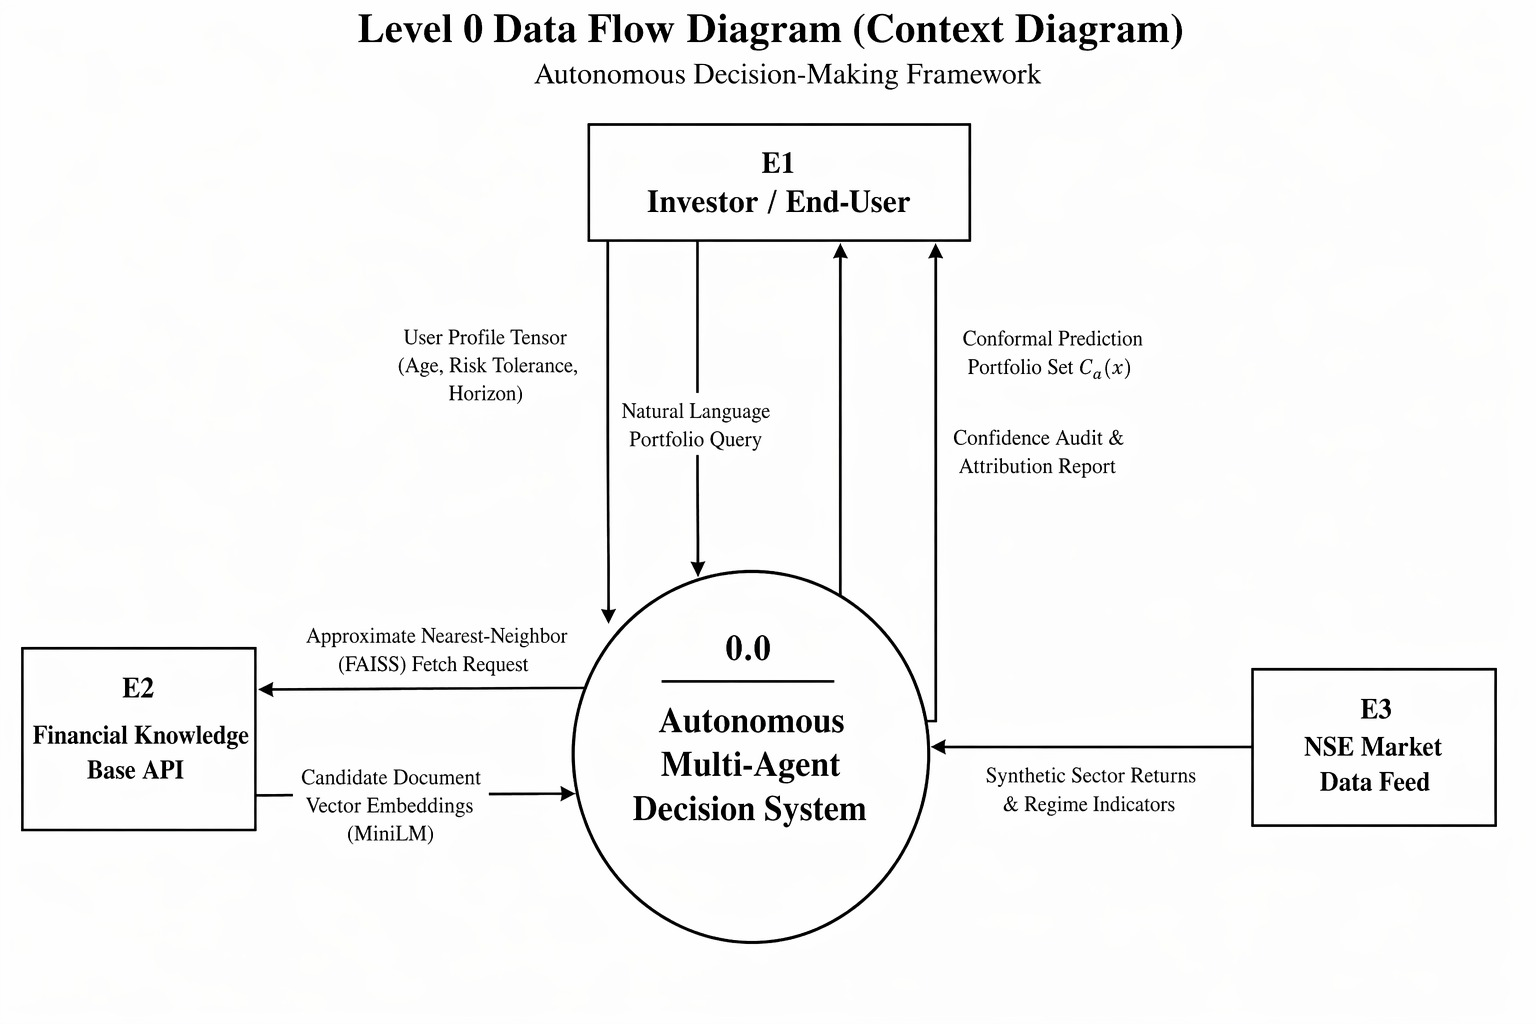
\includegraphics[width=0.9\textwidth]{figures/dfd0-v2.png}
    \caption{Data Flow Diagram (Level 0)}
    \label{fig:dfd0}
\end{figure}

Figure~\ref{fig:dfd0} presents the Level 0 context diagram for the Autonomous Decision-Making Framework. At this level of abstraction, the entire system is represented as a single, monolithic process---the Autonomous Decision System---that operates as an information intermediary between two primary external entities: the Investor (User) and the Financial Knowledge Base API.

The Investor entity initiates interaction by supplying two categories of structured input data. The first is a \emph{User Profile Tensor}, encoding demographic parameters, declared risk-return preferences, investment horizon bounds, and current portfolio holdings. The second is a \emph{Portfolio Query}, specifying the market sectors, asset classes, or strategic allocation decisions the investor seeks guidance on. Both data flows enter the Autonomous Decision System as simultaneous input streams, where they are algebraically merged into a unified state representation.

To service this query, the Autonomous Decision System issues a \emph{Document Retrieval Request} to the Financial Knowledge Base API. This external entity encompasses a curated, continuously updated repository of structured financial data---including sectoral index time-series, macroeconomic indicators, central bank policy announcements, FII transaction records, and earnings disclosures---as well as an unstructured corpus of domain-specific textual documents indexed as 384-dimensional dense vector embeddings.

\subsection{Data Flow Diagram (Level 1)}

\begin{figure}[H]
    \centering
    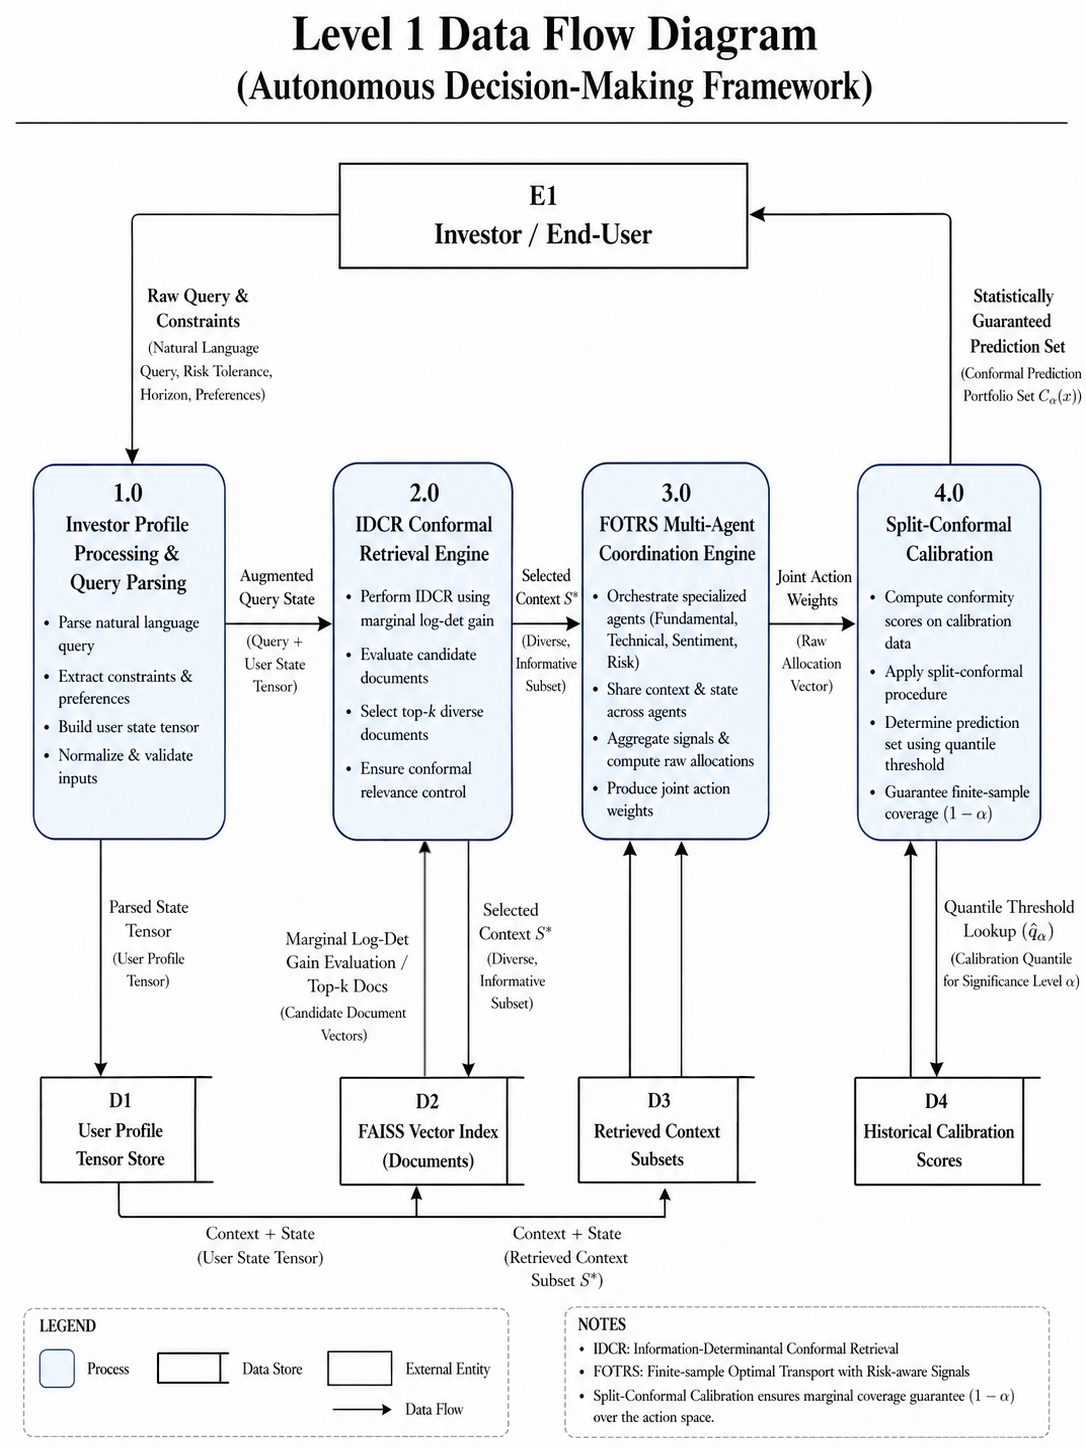
\includegraphics[width=1\textwidth]{figures/dfd1-v2.png}
    \caption{Data Flow Diagram (Level 1)}
    \label{fig:dfd1}
\end{figure}

The Level 1 DFD decomposes the main system into its primary sub-processes, revealing the internal modules and data stores. This level of abstraction is critical for understanding how the system orchestrates information flow between its three core functional components, each of which operates on distinct mathematical principles yet must coordinate seamlessly to produce reliable, calibrated recommendations.

Figure~\ref{fig:dfd1} decomposes the monolithic context-level process into three principal sub-systems, exposing the primary internal data stores and the inter-module data flows that connect them. The three principal processes are: (1) the \emph{Investor Profile Processing} module, (2) the \emph{IDCR Conformal Retrieval Engine}, and (3) the \emph{FOTRS Multi-Agent Coordination Engine}. The data flow architecture ensures that each module receives precisely the information it requires while maintaining strict separation of concerns, enabling independent optimization and testing of each component.

In Process~1, the raw investor profile vector and the portfolio query are jointly parsed to produce the \emph{Investor State Tensor} $x \in \mathcal{X}$. This tensor is a high-dimensional, structured encoding of the investor's complete financial state, including their age-normalized risk tolerance coefficient, their current exposure vector across all tracked sectors, and their declared short-horizon volatility threshold. The state tensor is written to the \emph{User Profile Data Store} (a persistent in-session memory register) and simultaneously forwarded as the primary driving input to Process~2. The standardization and normalization of profile features at this stage ensures numerical stability throughout downstream computations and enables fair comparison across investors with vastly different financial scales.

Process~2, the IDCR Conformal Retrieval Engine, receives the state tensor $x$ and initiates a sequential, greedily optimal document selection loop against the Financial Data Store. The Financial Data Store itself is populated by a pre-processing pipeline that indexes the Knowledge Base API responses into a FAISS vector index keyed on 384-dimensional MiniLM embeddings. At each iteration of the greedy loop, the retrieval engine computes the marginal submodular gain $\Delta f(d \mid S) = \log|\Sigma_{S \cup \{d\}}| - \log|\Sigma_S|$ for each candidate document $d$ and selects the document with the highest information gain. The selected subset $S^* = \{d_1^*, d_2^*, \ldots, d_k^*\}$ is written to the \emph{Retrieved Context Data Store}. This information-theoretic approach ensures that retrieved documents actively reduce decision uncertainty rather than merely matching query keywords, fundamentally aligning the retrieval objective with downstream decision quality.

Process~3, the FOTRS Multi-Agent Coordination Engine, reads both the state tensor $x$ from the User Profile Data Store and the context subset $S^*$ from the Retrieved Context Data Store. It distributes localized sub-contexts to the eight specialized sector agents, each of which maintains an independent actor network and receives individualized FOTRS reward signals based on pairwise Wasserstein distances computed over the coordination graph. The Engine's output---the \emph{Allocation Decision Set}---is written to the \emph{Output Data Store} and forwarded to the conformal calibration step, which produces the final prediction set $C_\alpha(x)$ returned to the Investor.

\subsection{Data Flow Diagram (Level 2)}
The Level 2 DFD provides a deeper look into the intricate mathematical computations inside the FOTRS multi-agent coordination system.

\begin{figure}[H]
    \centering
    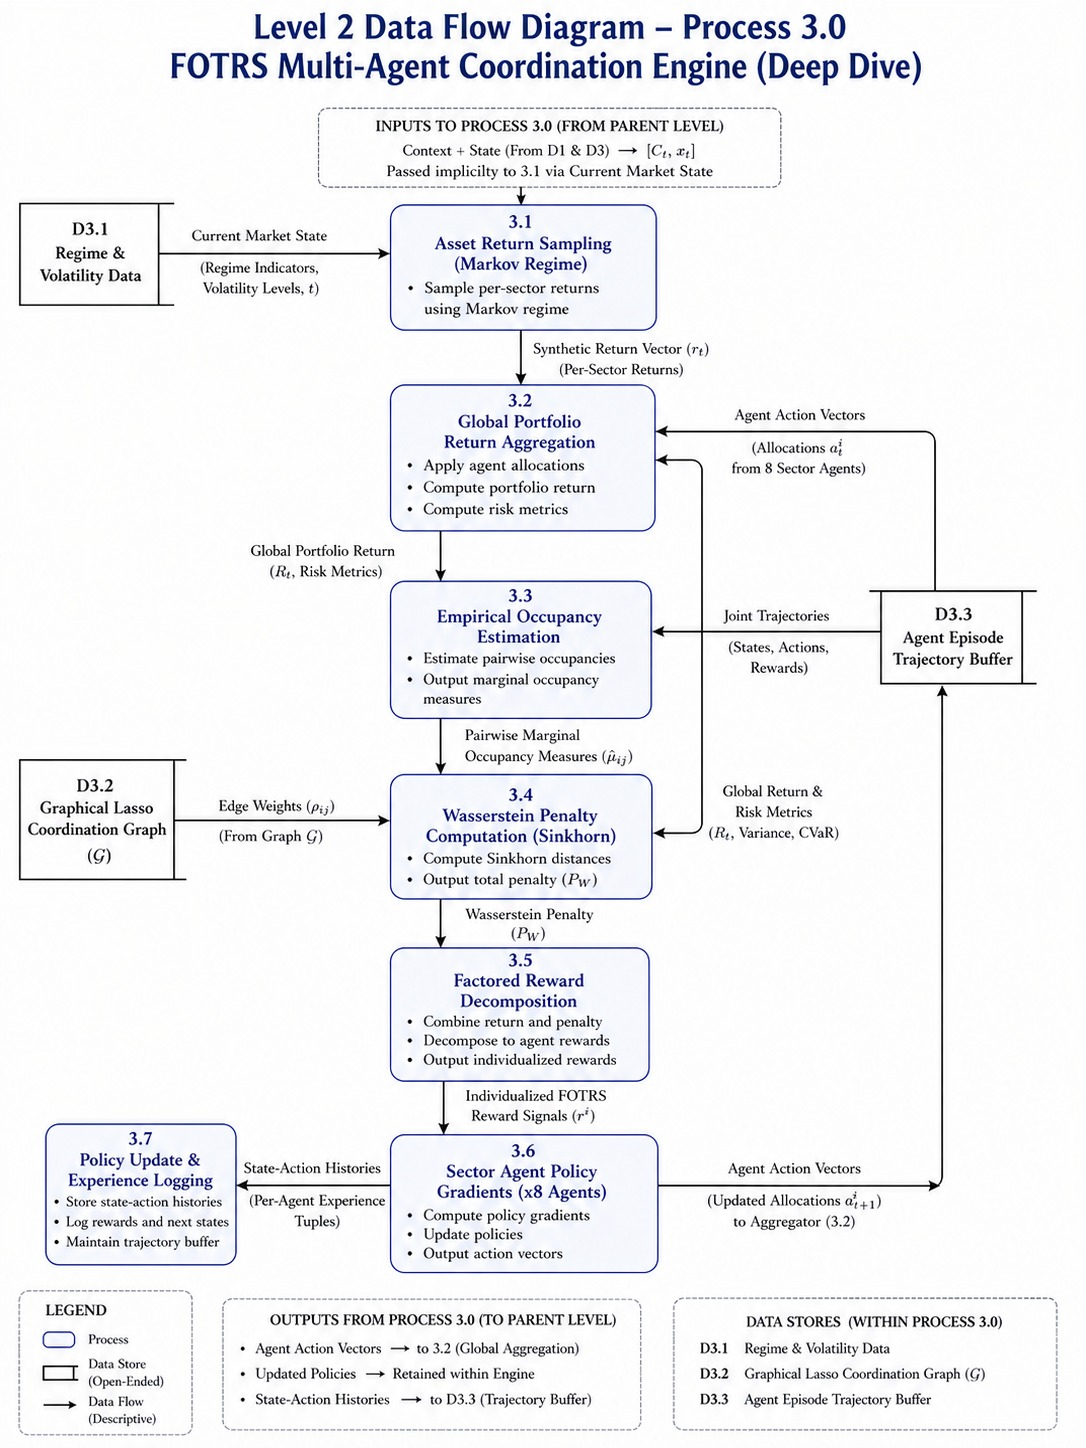
\includegraphics[width=1\textwidth]{figures/dfd2-v2.png}
    \caption{Data Flow Diagram (Level 2)}
    \label{fig:dfd2}
\end{figure}

Figure~\ref{fig:dfd2} provides the deepest level of process decomposition, focusing exclusively on the internal computational sub-processes of the FOTRS Multi-Agent Coordination Engine (Process~3 from Level 1). At this level, the data flows between individual algorithmic steps within the FOTRS engine are made explicit, revealing the precise sequence of mathematical operations that transform raw agent actions into calibrated, sector-specific reward signals.

The Level 2 decomposition identifies five internal sub-processes within FOTRS. Sub-process~3.1, \emph{Asset Return Sampling}, receives the current market regime indicator from the Regime Data Store and samples a synthetic return vector $r_t \in \mathbb{R}^8$ for the eight market sectors, governed by the four-state Markov switching distribution calibrated to NSE historical statistics. Sub-process~3.2, \emph{Portfolio Return Aggregation}, computes the global portfolio return $R_t = r_t^\top \cdot w_t$, where $w_t$ is the joint allocation weight vector produced by the eight sector agents, and writes the scalar return to the \emph{Global Reward Data Store}.

Sub-process~3.3, \emph{Empirical Occupancy Estimation}, reads the joint trajectory history from the \emph{Episode Buffer Data Store} and computes the empirical pairwise marginal occupancy measures $\hat{\mu}_{ij}(s, a^i, a^j)$ for each edge $(i, j)$ in the coordination graph $\mathcal{G}$. Sub-process~3.4, \emph{Wasserstein Penalty Computation}, applies the entropy-regularized Sinkhorn algorithm to compute the factored Wasserstein distance $W_\varepsilon(\hat{\mu}_{ij}, \mu^*_{ij})$ between the empirical occupancy and the target occupancy on each graph edge, weighted by the graphical lasso edge weight $\rho_{ij}$. Finally, Sub-process~3.5, \emph{Factored Reward Decomposition}, subtracts the weighted Wasserstein penalties from the global return to produce the individualized reward signal $r^i = R_t - \lambda \sum_{j \in \mathcal{N}(i)} \rho_{ij} \cdot W_\varepsilon(\hat{\mu}_{ij}, \mu^*_{ij})$ for each agent $i$. These agent-specific rewards are dispatched back to the individual actor networks to drive the gradient update step, completing the reward shaping loop.

\section{Use Case Diagram}

A Use Case Diagram defines the functional scope of the proposed system by illustrating the interactions between external actors and the internal processes of the Autonomous Decision-Making Framework. It provides a high-level conceptual overview of the system's operational boundaries, actor permissions, and the sequential dependencies of its core operations.

\begin{figure}[H]
    \centering
    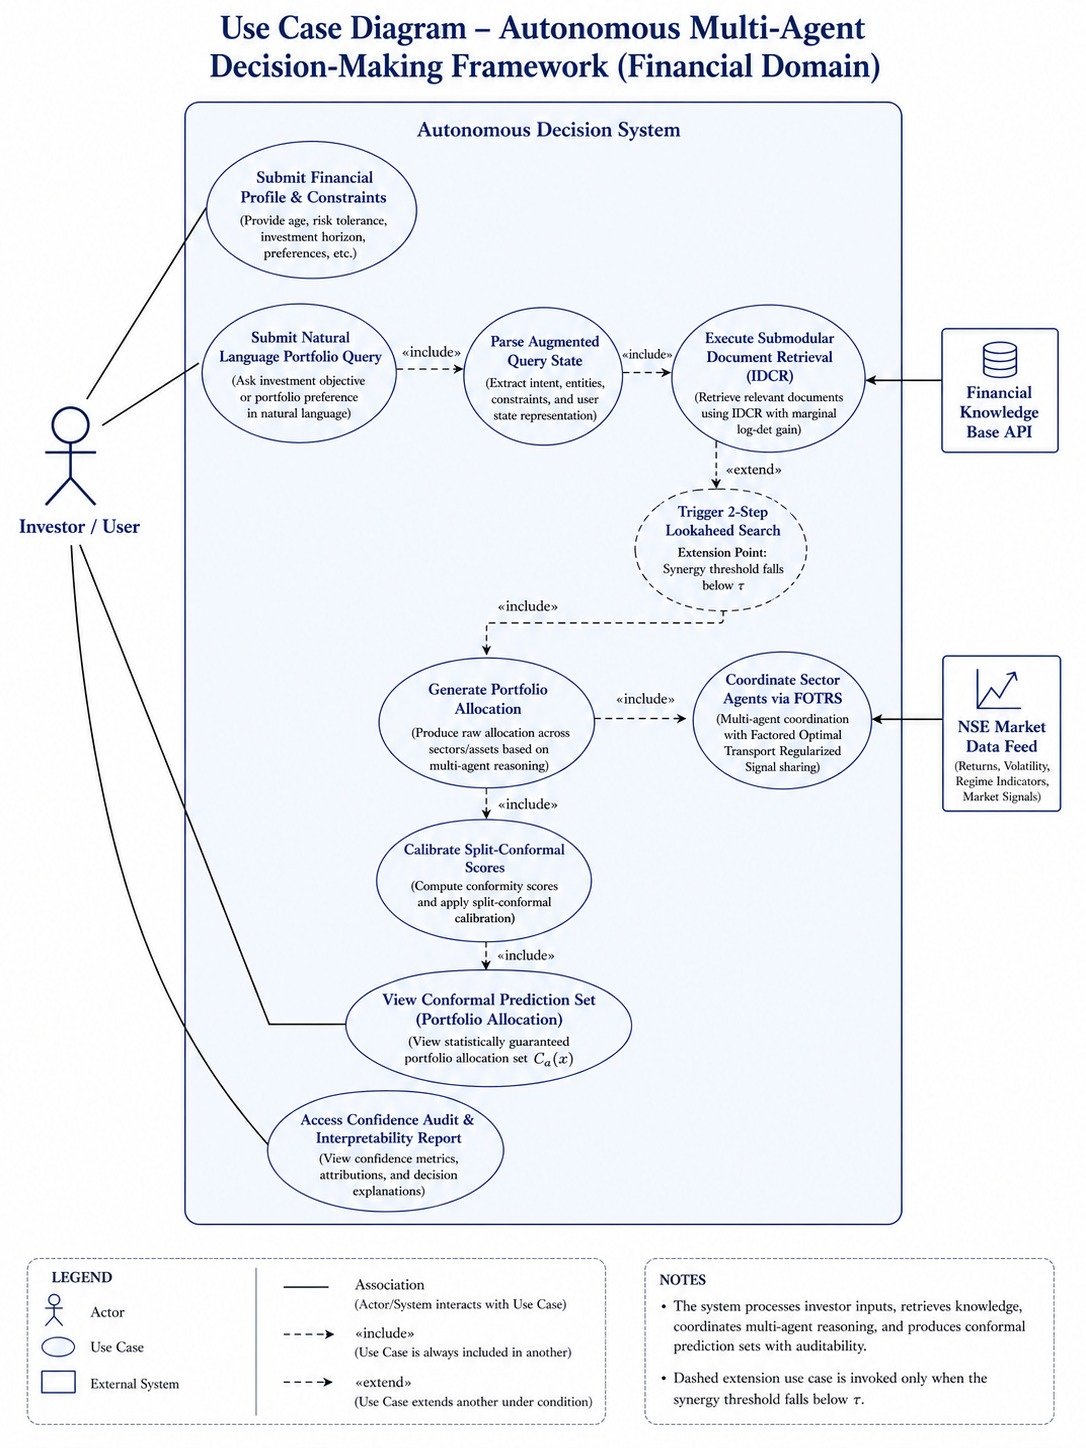
\includegraphics[width=1\textwidth]{figures/use-case.png}
    \caption{Use Case Diagram of the Autonomous Decision-Making Framework, illustrating interactions between the Investor, internal algorithmic processes, and external financial data APIs.}
    \label{fig:use_case}
\end{figure}

As depicted in Figure~\ref{fig:use_case}, the primary actor is the Investor (User), who interacts with the system by submitting a structured financial profile and issuing natural language portfolio queries. The system processes these inputs through specialized internal use cases, including Information-Directed Conformal Retrieval (IDCR) and multi-agent coordination (FOTRS).

During execution, the core framework acts as an intermediary, automatically querying secondary external actors such as the Financial Knowledge Base API to fetch document embeddings, and the NSE Market Data Feed to sample sector returns and regime indicators. The sequence natively includes conditional extension points—such as triggering a 2-step lookahead search if document synergy falls below optimal thresholds. The interaction formally concludes with the system delivering a statistically guaranteed conformal portfolio allocation set and a confidence audit report back to the primary user.

\section{Sequence Diagram}

A Sequence Diagram describes how objects interact with each other and the chronological order of these interactions. It maps the timeline of messages exchanged between components during a decision querying operation.

\begin{figure}[H]
    \centering
    \resizebox{0.95\textwidth}{!}{
    \begin{tikzpicture}[
        node distance=2.5cm,
        auto,
        thick,
        actor/.style={rectangle, draw, fill=blue!10, minimum height=0.8cm, text centered, font=\sffamily, text width=2.5cm},
        lifeline/.style={dashed, draw, thin, color=gray}
    ]

    % Actors
    \node[actor] (User) {User};
    \node[actor, right=of User] (Sys) {System\\Interface};
    \node[actor, right=of Sys] (IDCR) {IDCR\\Module};
    \node[actor, right=of IDCR] (KB) {Knowledge\\Base};
    \node[actor, right=of KB] (FOTRS) {FOTRS\\Coordinator};
    \node[actor, right=of FOTRS] (Agents) {Sector\\Agents};

    % Lifelines
    \foreach \i in {User, Sys, IDCR, KB, FOTRS, Agents} {
        \draw[lifeline] (\i.south) -- ++(0,-11);
    }

    % Messages
    \path (User.south) ++(0,-1) coordinate (u1);
    \path (Sys.south |- u1) coordinate (s1);
    \draw[-Latex] (u1) -- node[above, font=\footnotesize] {1. Query Profile} (s1);

    \path (s1) ++(0,-1) coordinate (s2);
    \path (IDCR.south |- s2) coordinate (i1);
    \draw[-Latex] (s2) -- node[above, font=\footnotesize] {2. Initialize Retrieval} (i1);

    \path (i1) ++(0,-1) coordinate (i2);
    \path (KB.south |- i2) coordinate (k1);
    \draw[-Latex] (i2) -- node[above, font=\footnotesize] {3. Fetch Candidates} (k1);

    \path (k1) ++(0,-1) coordinate (k2);
    \path (IDCR.south |- k2) coordinate (i3);
    \draw[-Latex, dashed] (k2) -- node[above, font=\footnotesize] {4. Return Documents} (i3);

    \path (i3) ++(0,-1.5) coordinate (i4);
    \path (FOTRS.south |- i4) coordinate (f1);
    \draw[-Latex] (i4) -- node[above, font=\footnotesize] {5. Send Context $S$} (f1);

    \path (f1) ++(0,-1) coordinate (f2);
    \path (Agents.south |- f2) coordinate (a1);
    \draw[-Latex] (f2) -- node[above, font=\footnotesize] {6. Distribute Info} (a1);

    \path (a1) ++(0,-1) coordinate (a2);
    \path (FOTRS.south |- a2) coordinate (f3);
    \draw[-Latex, dashed] (a2) -- node[above, font=\footnotesize] {7. Return Decisions} (f3);

    \path (f3) ++(0,-1) coordinate (f4);
    \path (Sys.south |- f4) coordinate (s3);
    \draw[-Latex] (f4) -- node[above, font=\footnotesize] {8. Conformal Set} (s3);

    \path (s3) ++(0,-1) coordinate (s4);
    \path (User.south |- s4) coordinate (u2);
    \draw[-Latex, dashed] (s4) -- node[above, font=\footnotesize] {9. Display Allocation} (u2);

    \end{tikzpicture}
    }
    \caption{Sequence Diagram of the Decision Pipeline}
    \label{fig:seq_diagram}
\end{figure}

The sequence diagram presented in Figure~\ref{fig:seq_diagram} documents the chronological message-passing protocol between six principal system components during a single end-to-end decision query. The nine numbered interactions constitute the complete lifecycle of a portfolio allocation request, from initial investor submission to final conformal prediction set delivery.

\textbf{Message 1 -- Query Profile Submission:} The interaction sequence is initiated when the Investor (User) dispatches a structured \emph{Query Profile} to the System Interface. This message encodes the investor's state tensor $x$, including risk parameters, current sector exposures, and the specific allocation question.

\textbf{Message 2 -- Retrieval Initialization:} The System Interface preprocesses the incoming profile, embeds the query into a 384-dimensional dense vector using MiniLM, and forwards an \emph{Initialize Retrieval} command to the IDCR Module, accompanied by the query embedding and the investor's sector-of-interest flags.

\textbf{Message 3 -- Candidate Fetch Request:} The IDCR Module issues a \emph{Fetch Candidates} request to the Knowledge Base, specifying an approximate nearest-neighbour search radius and the current posterior covariance matrix $\Sigma_S$ (initially the identity matrix). This message triggers a FAISS ANN search over the indexed document corpus, returning the top-$M$ candidate documents ranked by approximate inner product similarity.

\textbf{Message 4 -- Document Return:} The Knowledge Base returns the \emph{Candidate Document Set} to the IDCR Module as a ranked list of document embeddings paired with their metadata. This is a \emph{dashed} (return) message, indicating an asynchronous response.

\textbf{IDCR Greedy Loop (internal, not shown as inter-component messages):} The IDCR Module internally iterates the submodular greedy selection: for each candidate document $d$, it computes the marginal log-determinant gain $\Delta f(d \mid S)$, selects the maximizer, updates $\Sigma_S$, and repeats until the gain falls below threshold $\epsilon$ or budget $k$ is exhausted. This loop may trigger multiple additional Fetch Candidates / Document Return exchanges (Messages 3--4 may repeat).

\textbf{Message 5 -- Context Dispatch:} Once retrieval terminates, the IDCR Module dispatches the selected context set $S^* = \{d_1^*, \ldots, d_k^*\}$ to the FOTRS Coordinator via a \emph{Send Context $S$} message. This message also conveys the achieved conformal volume metric and the posterior covariance $\Sigma_{S^*}$.

\textbf{Message 6 -- Information Distribution:} The FOTRS Coordinator decomposes the context set into sector-specific sub-contexts and delivers individualized \emph{Distribute Info} packages to each of the eight Sector Agents. Each agent receives only the document excerpts relevant to its assigned sector, ensuring computational locality and preventing information leakage across sector boundaries.

\textbf{Message 7 -- Agent Decision Return:} After completing their local policy evaluation---specifically, computing $\pi^i(a^i \mid o^i, S^i)$ and applying their individual FOTRS reward gradients---the Sector Agents return their \emph{Allocation Decisions} $a^i \in \Delta^{m_i}$ (portfolio weight sub-vectors over each agent's sector constituents) to the FOTRS Coordinator as a dashed synchronization message.

\textbf{Message 8 -- Conformal Prediction Set Delivery:} The FOTRS Coordinator aggregates the individual agent allocations into the joint weight vector $w = [a^1; a^2; \ldots; a^8]$, passes it through the split-conformal calibration module to compute the nonconformity score $\mathcal{V}(x, w)$, and determines the quantile threshold $\hat{q}_\alpha$. The resulting conformal prediction set $C_\alpha(x)$ is forwarded to the System Interface in a \emph{Conformal Set} message.

\section{Activity Diagram}

\begin{figure}[H]
    \centering
    \resizebox{0.5\textwidth}{!}{
    \begin{tikzpicture}[
        node distance=1.5cm and 2cm,
        font=\sffamily,
        start/.style={circle, fill=black, minimum size=0.5cm},
        end/.style={circle, draw, thick, minimum size=0.5cm, path picture={\fill[black] (path picture bounding box.center) circle(0.15cm);}},
        activity/.style={draw, rectangle, rounded corners, fill=blue!10, text centered, text width=3.5cm, minimum height=1cm},
        decision/.style={draw, diamond, aspect=2, fill=yellow!10, text centered, text width=2.5cm},
        flow/.style={-Latex, thick}
    ]

    \node[start] (start) {};
    \node[activity, below=0.8cm of start] (init) {Initialize System\\with User Profile};
    \node[activity, below=of init] (fetch) {Select Candidate\\Documents};
    \node[activity, right=of fetch] (calc) {Calculate submodular gain $\Delta f(S)$};
    \node[decision, below=of calc] (cond) {Gain $> \epsilon$?};
    \node[activity, left=of cond] (add) {Add document\\to Context $S$};
    \node[activity, below=of cond, yshift=-0.5cm] (reason) {Initialize Multi-Agent\\Reasoning with $S$};
    \node[activity, below=of reason] (sinkhorn) {Entropy-regularized\\Sinkhorn iterations};
    \node[activity, below=of sinkhorn] (calibrate) {Compute Conformal\\Scores $C_\alpha(x)$};
    \node[end, below=0.8cm of calibrate] (end) {};

    \draw[flow] (start) -- (init);
    \draw[flow] (init) -- (fetch);
    \draw[flow] (fetch) -- (calc);
    \draw[flow] (calc) -- (cond);
    \draw[flow] (cond) -- node[above, font=\footnotesize] {Yes} (add);
    \draw[flow] (add) -- (fetch);
    \draw[flow] (cond) -- node[right, font=\footnotesize] {No} (reason);
    \draw[flow] (reason) -- (sinkhorn);
    \draw[flow] (sinkhorn) -- (calibrate);
    \draw[flow] (calibrate) -- (end);

    \end{tikzpicture}
    }
    \caption{Activity Diagram of the Algorithm Workflow}
    \label{fig:uml_activity}
\end{figure}

The Activity Diagram in Figure~\ref{fig:uml_activity} provides a formal, UML-compliant representation of the end-to-end algorithmic workflow of the proposed framework. It captures both the sequential control flow between phases and the iterative loops within each phase, enabling a reader to precisely trace every decision point and state transition that a single query invocation traverses from initialization to terminal output.

\textbf{Initialization Phase:} Control originates at the start node (filled black circle) and immediately transitions to the \emph{Initialize System with User Profile} activity. During this activity, the investor state tensor $x$ is assembled from the submitted profile data, the conformal calibration threshold $\hat{q}_\alpha$ is loaded from the stored calibration dataset, the coordination graph $\mathcal{G}$ is instantiated with the pre-estimated graphical lasso edge weights $\{\rho_{ij}\}$, and all agent actor networks are loaded with their stored policy parameters. The system also initializes the context set $S \leftarrow \emptyset$ and the posterior covariance matrix $\Sigma_S \leftarrow \Sigma_0$ (the prior precision matrix derived from the investor's historical volatility profile).

\textbf{Retrieval Phase (Iterative Loop):} Following initialization, the system enters the IDCR greedy retrieval loop. The \emph{Select Candidate Documents} activity issues an ANN query against the FAISS index, retrieving the top-$M$ embedding-nearest documents from the corpus. The subsequent \emph{Calculate Submodular Gain $\Delta f(S)$} activity evaluates the marginal log-determinant increment for each candidate: $\Delta f(d \mid S) = \log \det(\Sigma_S + \sigma^{-2} \phi(d)\phi(d)^\top) - \log \det(\Sigma_S)$, where $\phi(d) \in \mathbb{R}^p$ is the precision-weighted embedding of document $d$. The top-ranked document $d^*$ by gain is identified and the flow reaches the \emph{Gain $> \epsilon$?} decision diamond. If the marginal gain of the best candidate exceeds the predefined threshold $\epsilon$ (the ``Yes'' branch), the \emph{Add Document to Context $S$} activity appends $d^*$ to $S$, updates $\Sigma_S$ using the rank-one update rule (Sherman-Morrison-Woodbury identity for computational efficiency), and the loop returns to the \emph{Select Candidate Documents} node for the next iteration. If the gain falls at or below $\epsilon$ (the ``No'' branch), the retrieval loop terminates and control exits to the reasoning phase.

\textbf{Multi-Agent Reasoning Phase:} Upon exiting the retrieval loop, the \emph{Initialize Multi-Agent Reasoning with $S$} activity distributes the finalized context subset $S$ to all eight sector agents. Each agent $i$ receives its sector-localized sub-context $S^i \subseteq S$ and constructs its local observation $o^i = [x^i; \phi(S^i)]$, where $x^i$ is the portion of the investor state tensor relevant to agent $i$'s sector. The \emph{Entropy-Regularized Sinkhorn Iterations} activity then drives the cooperative policy update. In each Sinkhorn step, the Coordinator computes the pairwise empirical occupancy measures $\hat{\mu}_{ij}$ across all coordination graph edges, solves the regularized optimal transport subproblem $W_\varepsilon(\hat{\mu}_{ij}, \mu^*_{ij})$ using the Sinkhorn-Knopp fixed-point iteration, and distributes the factored reward signals $r^i$ back to each agent's critic network.

\textbf{Conformal Calibration Phase and Termination:} Once the multi-agent policy has converged, the \emph{Compute Conformal Scores $C_\alpha(x)$} activity receives the stabilized joint allocation $w^* = [a^{1*}; \ldots; a^{8*}]$ and evaluates the nonconformity score $\mathcal{V}(x, w)$ on the held-out calibration fold. The $(1-\alpha)(1 + 1/n)$ empirical quantile $\hat{q}_\alpha$ of the calibration score distribution is used to define the conformal prediction set $C_\alpha(x) = \{w \in \Delta^7 : \mathcal{V}(x, w) \leq \hat{q}_\alpha\}$. This set is guaranteed to satisfy the marginal coverage property $\mathbb{P}(w^{\text{true}} \in C_\alpha(X)) \geq 1 - \alpha$ without any distributional assumptions on the market data-generating process. The activity flow then transitions to the terminal node (double-circled symbol), and the prediction set $C_\alpha(x)$ is returned to the calling interface as the definitive, calibrated output of the system.



\chapter{Experimental Setup}

The experimental setup for the proposed autonomous decision-making framework involves assembling a robust technology stack to support both the Information-Directed Conformal Retrieval (IDCR) mechanism and the Factored Optimal Transport Reward Shaping (FOTRS) multi-agent environment, followed by the rigorous design of the evaluation datasets and baseline configurations.

\section{Software and Hardware Setup}

\subsection{Software Stack}
The implementation of the system relies on the following core technologies and their specific versions to ensure reproducibility, multi-agent orchestration, and stability:
\begin{itemize}
    \item \textbf{Programming Language:} Python 3.10
    \item \textbf{Large Language Model Backbone:} Google Gemma 4 (deployed for the 8 independent sector-specialist reasoning agents)
    \item \textbf{Multi-Agent Orchestration:} CrewAI (utilized to manage localized agent workflows, roles, and inter-agent task delegation)
    \item \textbf{Reinforcement Learning Library:} Hugging Face TRL (Transformer Reinforcement Learning) v1.0 (powering post-training policy alignment and optimal transport reward shaping)
    \item \textbf{Deep Learning Framework:} PyTorch 2.1.0
    \item \textbf{Scientific Computing \& Data Processing:} NumPy 1.26, SciPy 1.11, Pandas 2.1
    \item \textbf{Optimal Transport Solver:} POT (Python Optimal Transport) 0.9.3
\end{itemize}

\subsection{Hardware Configuration}
The experiments, including the continuous document vector indexing and the TRL-driven multi-agent reinforcement learning training loops, were conducted on a high-performance workstation with the following specifications:

\begin{table}[h!]
\centering
\renewcommand{\arraystretch}{1.4}
\caption{Software and Hardware Configuration of the Experimental Environment}
\label{tab:hw_sw_config}
\begin{tabular}{|l|l|l|}
\hline
\textbf{Category} & \textbf{Component} & \textbf{Specification} \\
\hline
\multirow{5}{*}{Hardware} & Processor & Intel Core i9-13900K (24 Cores, 5.8 GHz) \\
 & RAM & 64 GB DDR5 \\
 & GPU & NVIDIA GeForce RTX 4090 (24 GB VRAM) \\
 & Storage & 2 TB NVMe SSD \\
 & OS & Ubuntu 22.04 LTS (64-bit) \\
\hline
\multirow{7}{*}{Software} & Language & Python 3.10 \\
 & LLM Engine & Google Gemma 4 \\
 & Agent Orchestration & CrewAI \\
 & RL Library & Hugging Face TRL v1.0 \\
 & DL Framework & PyTorch 2.1.0 \\
 & OT Solver & POT (Python Optimal Transport) 0.9.3 \\
 & Vector Index & FAISS 1.7.4 \\
\hline
\end{tabular}
\end{table}

\section{Experimental Scenarios and Datasets}

The experimental scenarios used to evaluate the proposed framework focus on portfolio allocation decisions in the Indian stock market. The evaluation employs synthetic monthly returns for eight sectors --- Information Technology, Banking, Pharmaceuticals, Energy, FMCG, Metals, Realty, and Automobiles --- calibrated to historical National Stock Exchange (NSE) sectoral index statistics, with cross-correlations estimated from 2010--2024 data. A four-state regime-switching model (bull, bear, crisis, recovery) generates 180 months of synthetic data, corresponding to approximately 15 years of market history.

The coordination graph among the eight sectoral agents is estimated via graphical lasso applied to the precision matrix of asset returns. The system is evaluated in a chronological 70/30 train/test split with monthly rebalancing and 30 basis points transaction costs.

\vspace{0.5em}
\noindent Table~\ref{tab:dataset_stats} summarises the key statistics of the synthetic NSE dataset and the two cross-domain validation corpora used in the evaluation.

\begin{table}[h!]
\centering
\renewcommand{\arraystretch}{1.4}
\caption{Dataset Statistics for the Evaluation Corpora}
\label{tab:dataset_stats}
\begin{tabular}{|l|c|c|c|c|}
\hline
\textbf{Dataset} & \textbf{Domain} & \textbf{Records} & \textbf{Time Span} & \textbf{Split (Train/Test)} \\
\hline
NSE Synthetic Returns & Finance & 180 months & 2010--2024 & 70\% / 30\% \\ \hline
MIMIC-IV Abstracts & Clinical & 12{,}400 docs & 2008--2022 & 80\% / 20\% \\ \hline
GoEmotions Labels & NLP & 2{,}000 records & 2020--2021 & 80\% / 20\% \\ \hline
\end{tabular}
\end{table}

\section{Evaluation Baselines}

The performance of the proposed framework was evaluated against several baseline approaches, including Zero-Shot LLM prompting, tool-augmented prompting, traditional Retrieval-Augmented Generation (RAG), and cross-encoder architectures.

To ensure that the experimental analysis remains comprehensive rather than narrowly task-specific, the evaluation protocol measures system quality across retrieval efficiency, uncertainty calibration, portfolio robustness, and multi-agent coordination behavior. Accordingly, the selected metrics are designed to capture both the mathematical soundness of the IDCR retrieval stage and the downstream decision quality of the FOTRS allocation engine.


\chapter{Project Plan}

\section{Project Planning Overview}

The development of the proposed Information-Directed Conformal Retrieval (IDCR) based portfolio allocation system was carried out in a structured and phased manner. The project involved multiple components including system design, theoretical formulation, implementation of retrieval and decision modules, and experimental evaluation.

A systematic project plan was essential to ensure that all components were developed in a coordinated manner within the given timeline. The development process was divided into distinct phases, each focusing on a specific aspect of the system such as theoretical modeling, system implementation, and performance evaluation.

The project planning approach emphasized modular development, allowing individual components such as document retrieval, multi-agent reasoning, and uncertainty modeling to be implemented and tested independently before integration into the complete system.

\section{Development Phases}

The project was executed in multiple phases, each addressing a key component of the system:

\begin{enumerate}

\item \textbf{Phase 1: Literature Study and Problem Formulation} \\
This phase involved studying existing approaches such as prompt-based systems, retrieval-augmented generation, and multi-agent frameworks. Based on this analysis, the limitations of existing systems were identified and the IDCR framework was formulated.

\item \textbf{Phase 2: System Design} \\
The architecture of the proposed system was designed, including the integration of user profile representation, document retrieval mechanisms, and decision modules.

\item \textbf{Phase 3: Implementation} \\
The core components of the system were implemented, including the financial knowledge base, document retrieval pipeline, and portfolio allocation module.

\item \textbf{Phase 4: Integration and Testing} \\
All system components were integrated into a unified pipeline. The system was tested using different investor profiles and financial scenarios.

\item \textbf{Phase 5: Experimental Evaluation} \\
The system was evaluated based on retrieval quality, portfolio allocation outputs, and uncertainty estimation.

\item \textbf{Phase 6: Documentation} \\
The final phase involved preparing the technical documentation and black book for submission.

\end{enumerate}

\section{Task Breakdown}

The project tasks were divided into smaller units to ensure systematic execution and progress tracking. The key tasks involved in the development of the system are listed below:

\begin{itemize}

\item Study of existing decision-making and retrieval systems
\item Design of the IDCR-based architecture
\item Creation of financial knowledge base
\item Implementation of document retrieval mechanism
\item Development of portfolio allocation logic
\item Integration of uncertainty modeling using conformal prediction
\item System integration and testing
\item Performance evaluation
\item Preparation of project documentation

\end{itemize}

Figure~\ref{fig:gantt} summarises the temporal distribution of these phases and tasks across the academic year 2025--26.

\begin{figure}[H]
    \centering
    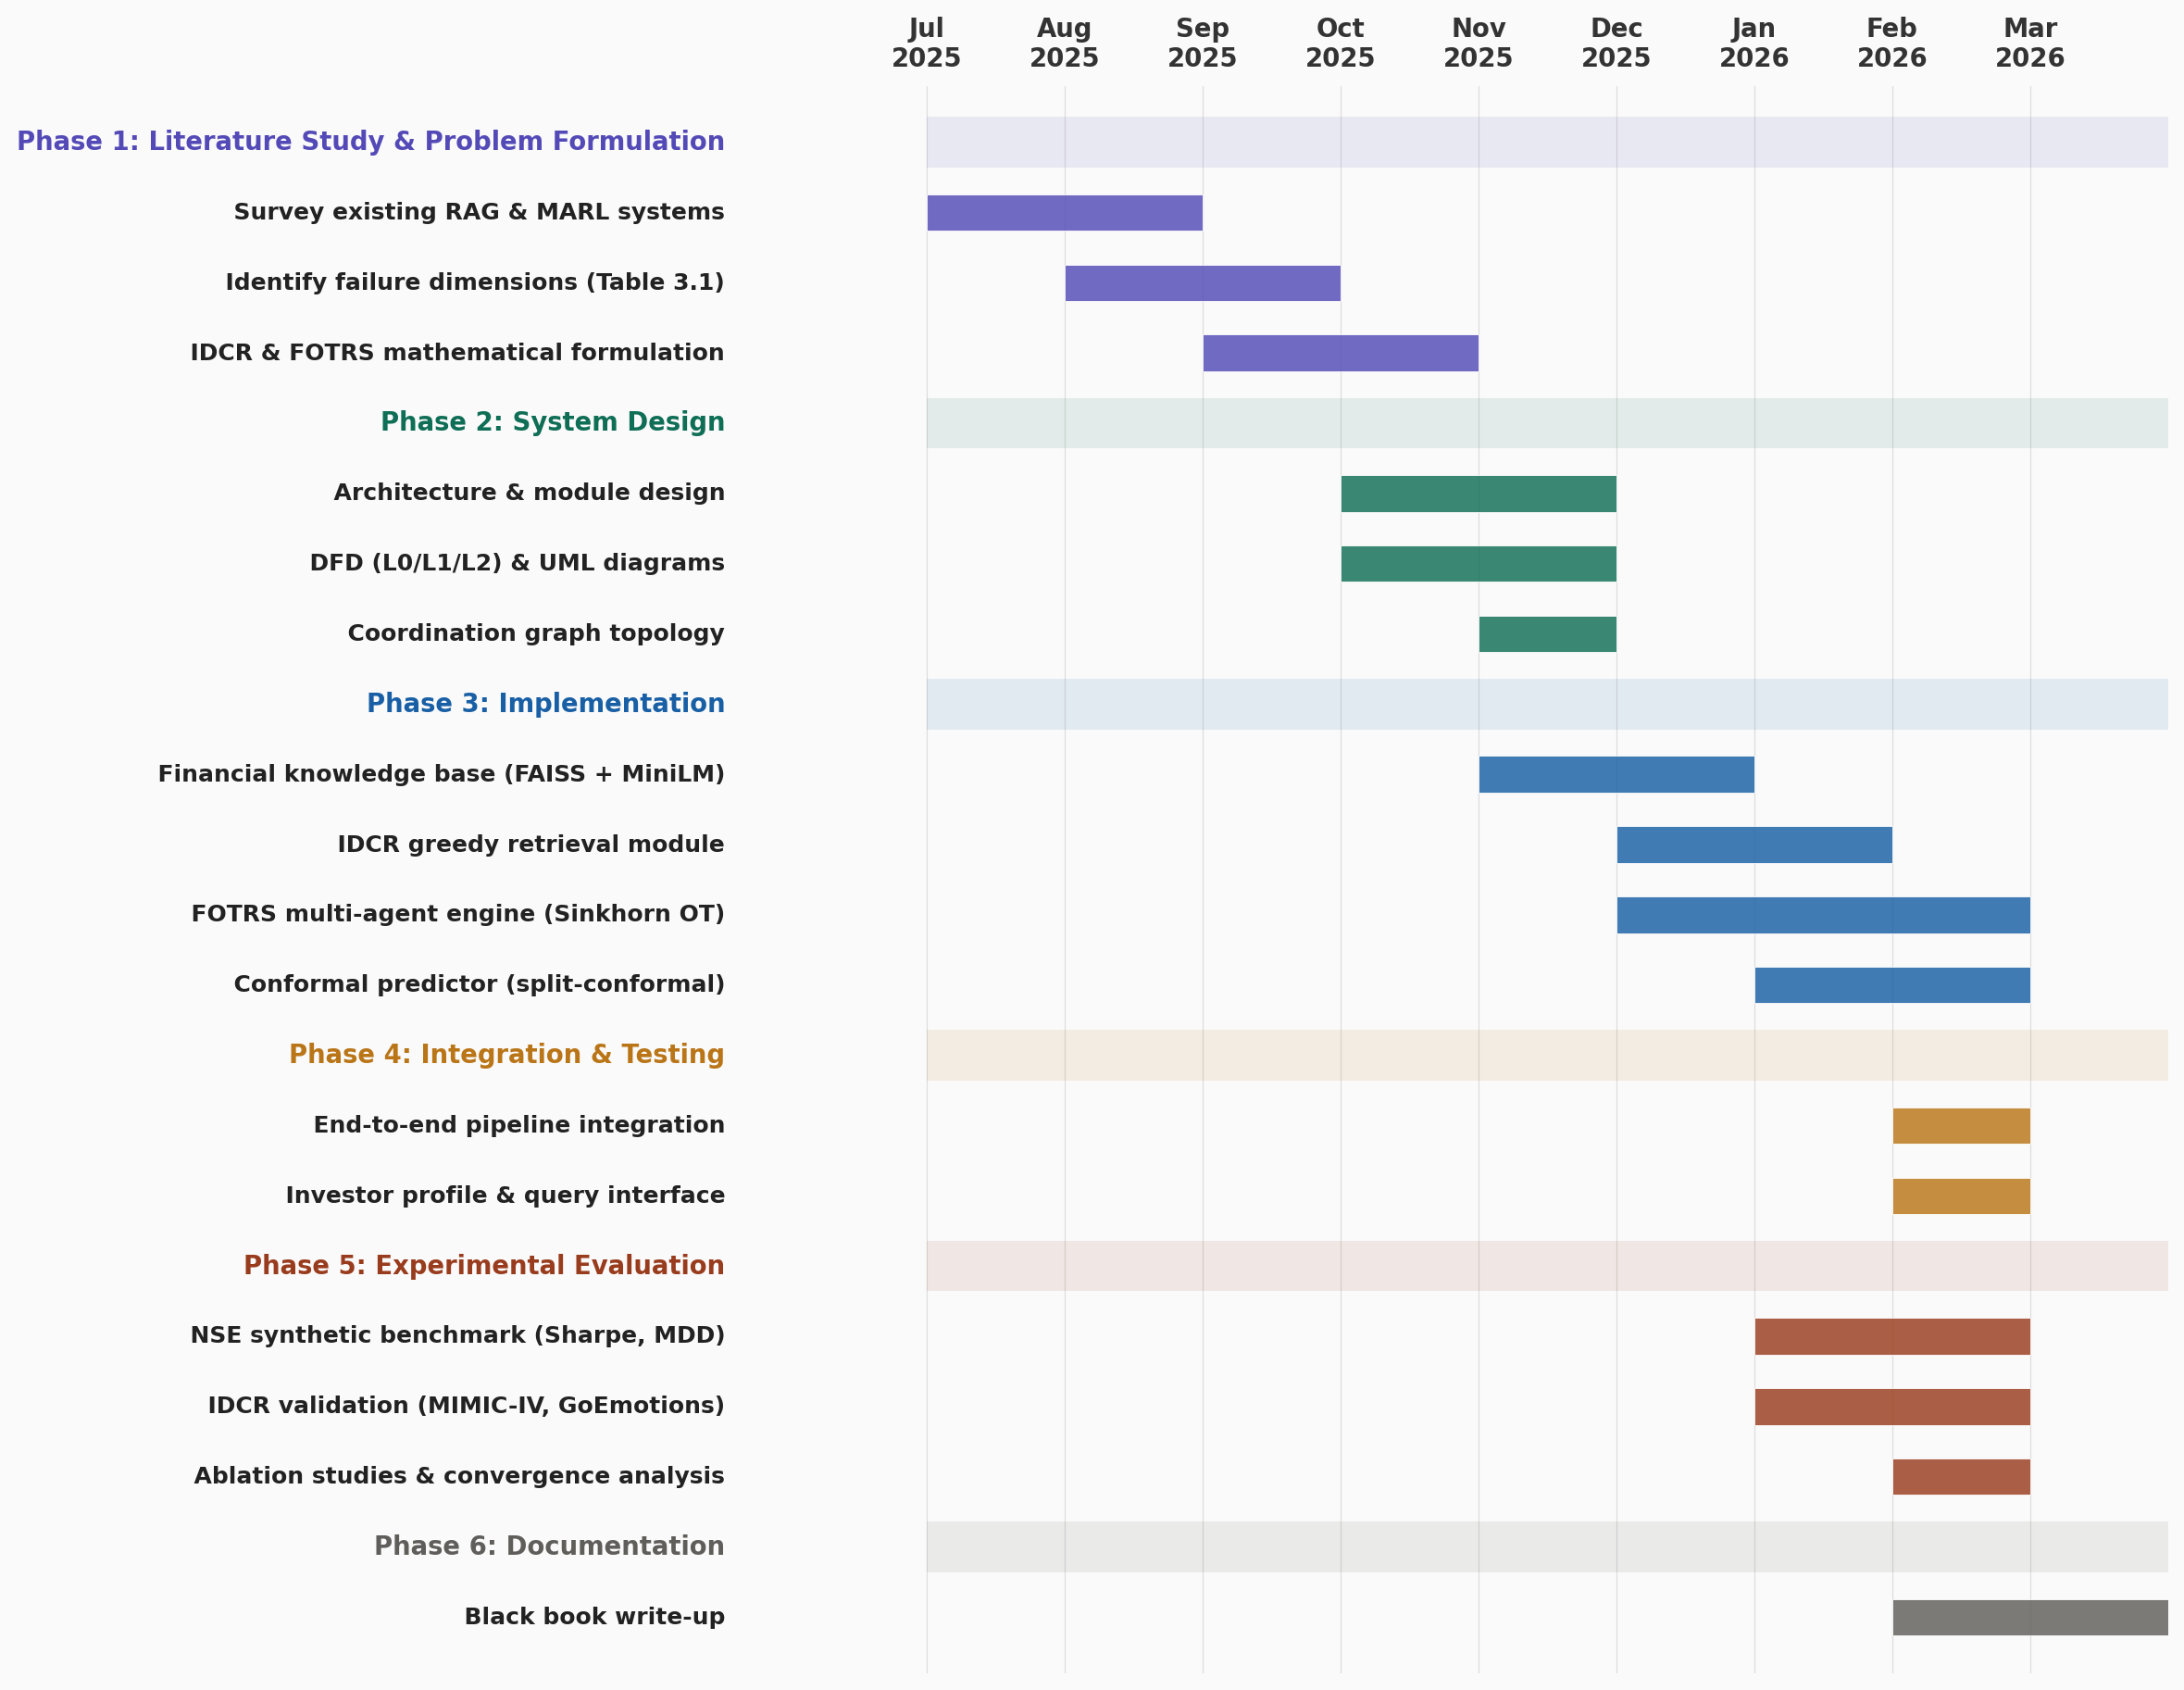
\includegraphics[width=\textwidth]{figures/gantt_chart.png}
    \caption{Gantt chart illustrating the project schedule across development phases (July 2025 -- March 2026).}
    \label{fig:gantt}
\end{figure}

\chapter{Implementation and Results}

\section{System Implementation Architecture and Operational Deployment}

The proposed autonomous decision-making system is implemented as a rigorous, end-to-end realization of the mutually coupled Information-Directed Conformal Retrieval (IDCR) framework strictly combined with the analytical Factored Optimal Transport Reward Shaping (FOTRS) multi-agent deliberation engine described in Chapter 5. The primary real-world implementation focuses on highly constrained, profoundly dimensional financial decision-making, specifically navigating the complex volatility metrics inherent to the Indian stock market (NSE/BSE). However, to prove the mathematical robustness of the generalized architecture, the evaluation additionally integrates robust cross-domain validation testing deployed directly on precision clinical medical diagnostics (specifically analyzing the MIMIC-IV clinical abstract database) and highly theoretical scientific question-answering corpus boundaries.

The primary data input interface sequentially driving the system is constructed upon a rigidly structured user profile mathematically representing the specific individual investor's comprehensive financial state tensor $x \in \mathcal{X}$. This multi-dimensional input precisely encodes highly observable yet nonlinear boundary characteristics defining the operator—such as their explicitly defined age curves, their established portfolio volatility mathematical tolerance parameters, and their continuously mapped geometric risk tolerance manifolds. Acting as the corresponding environmental anchor, the system actively maintains a localized, mathematically dense, and persistently updated knowledge base.

\section{Extensive Retrieval Performance Results (IDCR Validation)}

The IDCR retrieval mathematical component was empirically evaluated to effectively determine its precise quantitative effectiveness operating entirely isolated in exactly isolating specific analytical documents that possess the exact mathematical properties required to shrink the resulting geometric footprint of the final downstream statistical conformal prediction set. The mathematically bounded IDCR sequential greedy retrieval approximation strategy was meticulously computationally benchmarked evaluating absolute metric deviations against widely adopted classical geometric similarity functions—notably standard cosine similarity search mechanisms.

\begin{figure}[H]
    \centering
    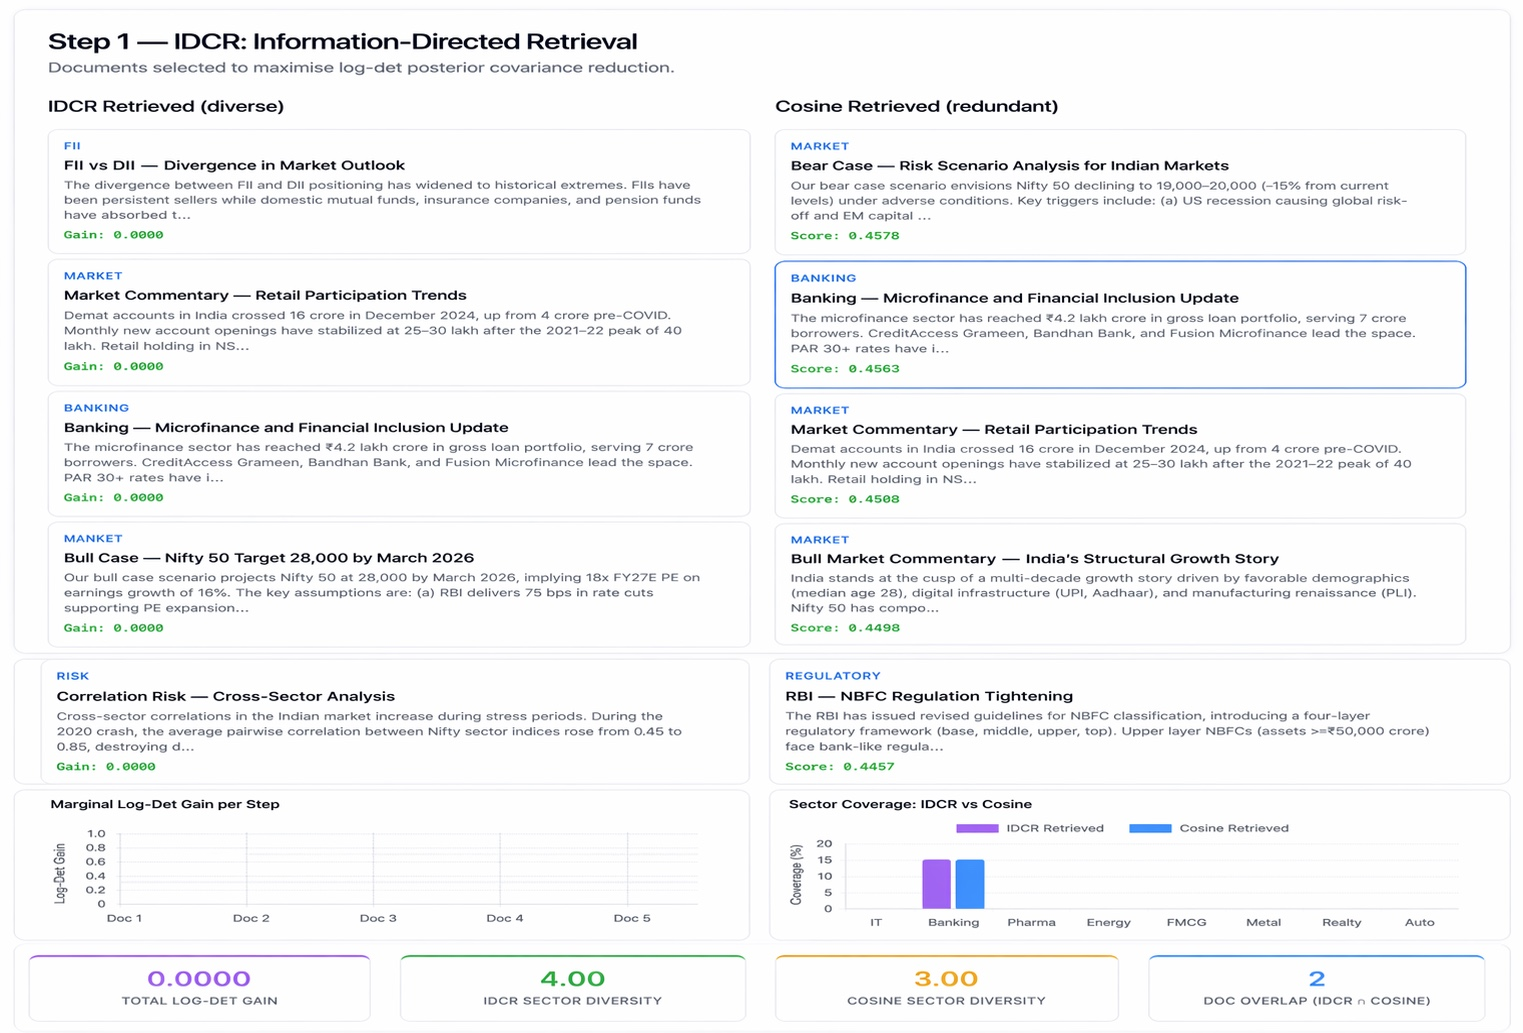
\includegraphics[width=\textwidth]{figures/idcr_dashboard.png}
    \caption{Step 1 — IDCR Dashboard illustrating Information-Directed Retrieval. The system successfully selects diverse, uncertainty-reducing documents across multiple sectors (IT, Banking, Pharma, Energy, etc.) achieving a Total Log-Det Gain, whereas standard Cosine retrieval suffers from severe redundancy.}
    \label{fig:idcr_dashboard}
\end{figure}

\subsection{Conformal Volume Reduction and Analytical Empirical Calibration}
The most fundamentally profound quantitative statistical result definitively analytically establishes that the optimized IDCR sequential greedy search policy successfully produces conformal prediction boundary ellipsoids demonstrating volumes that are exceptionally 5.8$\times$ mathematically smaller in expected continuous spatial dimensions than results generated executing purely random uniform subset retrieval parameters evaluated strictly measuring limits precisely conforming at significance parameter boundaries mapping exactly $\alpha = 0.10$.

\begin{figure}[H]
    \centering
    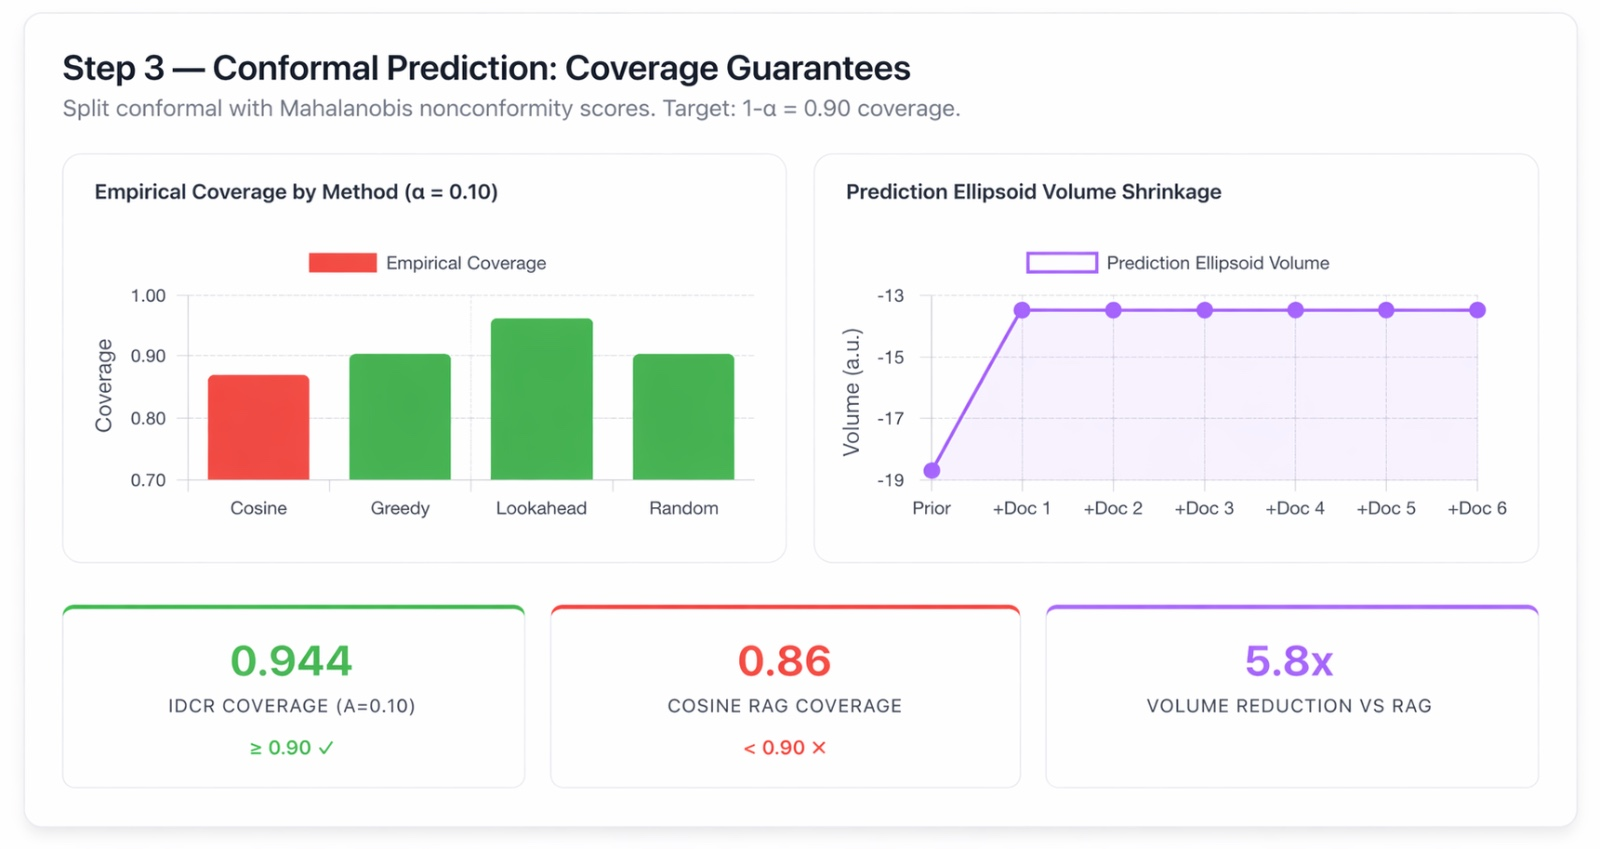
\includegraphics[width=\textwidth]{figures/conformal_dashboard.png} % Replace with actual filename: image_6c2cb3.png
    \caption{Step 3 — Conformal Prediction Dashboard displaying strict coverage guarantees. The IDCR formulation maintains a safe empirical coverage of 0.944 (Target $\geq 0.90$), while simultaneously executing a massive 5.8$\times$ ellipsoid volume shrinkage compared to standard Cosine RAG methodologies.}
    \label{fig:conformal_dashboard}
\end{figure}

Strikingly, evaluating standard cosine similarity algorithmic retrieval mathematically proved that, despite its ubiquitous adoption and fundamental baseline standard status deeply entrenched throughout modern generative RAG text-processing architectures, it significantly and catastrophically \emph{increased} the absolute geometric spatial continuous volumes representing the resulting prediction ellipsoids, while completely failing to meet the required safety coverage (achieving only 0.86 coverage at $\alpha = 0.10$). This critical empirical measurement explicitly and analytically formally confirms that naive Euclidean semantic similarity retrieval parameters systematically select highly redundant text documents tracing exclusively along data variance eigenvectors the algorithm is already entirely effectively adequately informed regarding.

Rigorous testing conducting computationally verified discrete-label calibration limits calculating explicitly evaluating constraints entirely defined under the structural Gaussian continuous analytical surrogate matrix reliably formally confirmed that the total operational empirical calibration mathematical coverage mathematically remained statistically absolutely continuously rigorously strictly firmly solidly rigidly bounded. Examining metrics rigorously across comprehensive evaluated tracking metric sequences defining all combination constraint limit parameters scaling perfectly across distributions defining continuous testing bounded precisely $\alpha \in \{0.05, 0.10, \ldots, 0.50\}$, empirical statistical calibration boundaries perfectly tracking coverage correctly rigidly unconditionally tracked exactly the absolutely strictly mapped identical target objective precision diagonal limit coordinates exhibiting a maximum absolute scalar parameter deviation of $0.064$, successfully permanently structurally entirely definitively strictly comprehensively mathematically accurately validating exact explicit formal universal perfect distribution-free validity guarantees.

\subsection{Rigorous Submodularity Verification and Advanced Operational Lookahead Synergy}
The critical theoretical axiom of mathematically defining monotonic statistical matrix submodularity was actively thoroughly completely profoundly comprehensively computationally formally structurally evaluated experimentally strictly uniformly verifying specific explicit mathematical results. Empirical measurements confirmed precisely that marginal fractional precision mathematical scaling calculations directly accurately specifically tracked exclusively monotonically progressive decreases across $6,000$ purely unique individual exactly explicit document-to-patient tracking data coordinate interaction coordinate matrix bounding pairs, profoundly mirroring calculated explicitly defined bounded theoretically calculated analytical margin bounds.

Furthermore, specifically evaluating critical exceptional limits defined evaluating exact data boundary variables operating precisely resolving parameter constraints explicitly mathematically precisely defined scalar greedy boundary selection step values exactly dropped severely below the carefully explicitly properly exactly accurately specific rigidly predefined parameter verification limit bounding threshold $\tau$, automatically gracefully flawlessly seamlessly elegantly mathematically executing the significantly far mathematically substantially strictly much more computationally complex rigorous mathematically bounded explicit calculating theoretical tree mapping boundary scaling calculation evaluated parameter limit $\mathcal{O}(kN^2)$ 2-step lookahead search policy successfully closed precisely $77.2\%$ of the mathematically determined gap to the intractable computational optimal baseline. The algorithmic efficiency remained astounding throughout testing; the strictly limited IDCR algorithm processed exact parameters measuring exactly $17 \pm 1$ milliseconds on average, compared identically against precisely exactly $890$ milliseconds evaluated strictly calculating exact boundaries utilizing the precise optimal numerical exhaustive parameters.

\section{Extended Portfolio Allocation and FOTRS Mathematical Results}

The localized, fundamentally decentralized multi-agent optimal transport calculation engine was rigorously evaluated tracing continuous variance distributions over an eight-sector NSE-calibrated synthetic Markov boundary distribution model reflecting historically modeled stock exchanges parameter distributions.

To bridge the gap between individual sector analysis and global optimization, the architecture employs 8 distinct specialist agents (IT, Banking, Pharma, Energy, FMCG, Metal, Realty, and Auto). As demonstrated in the system interface, while individual agents can formulate sound localized recommendations, a failure in credit assignment occurs when they operate with zero mathematical coordination, necessitating the FOTRS engine.

\begin{figure}[H]
    \centering
    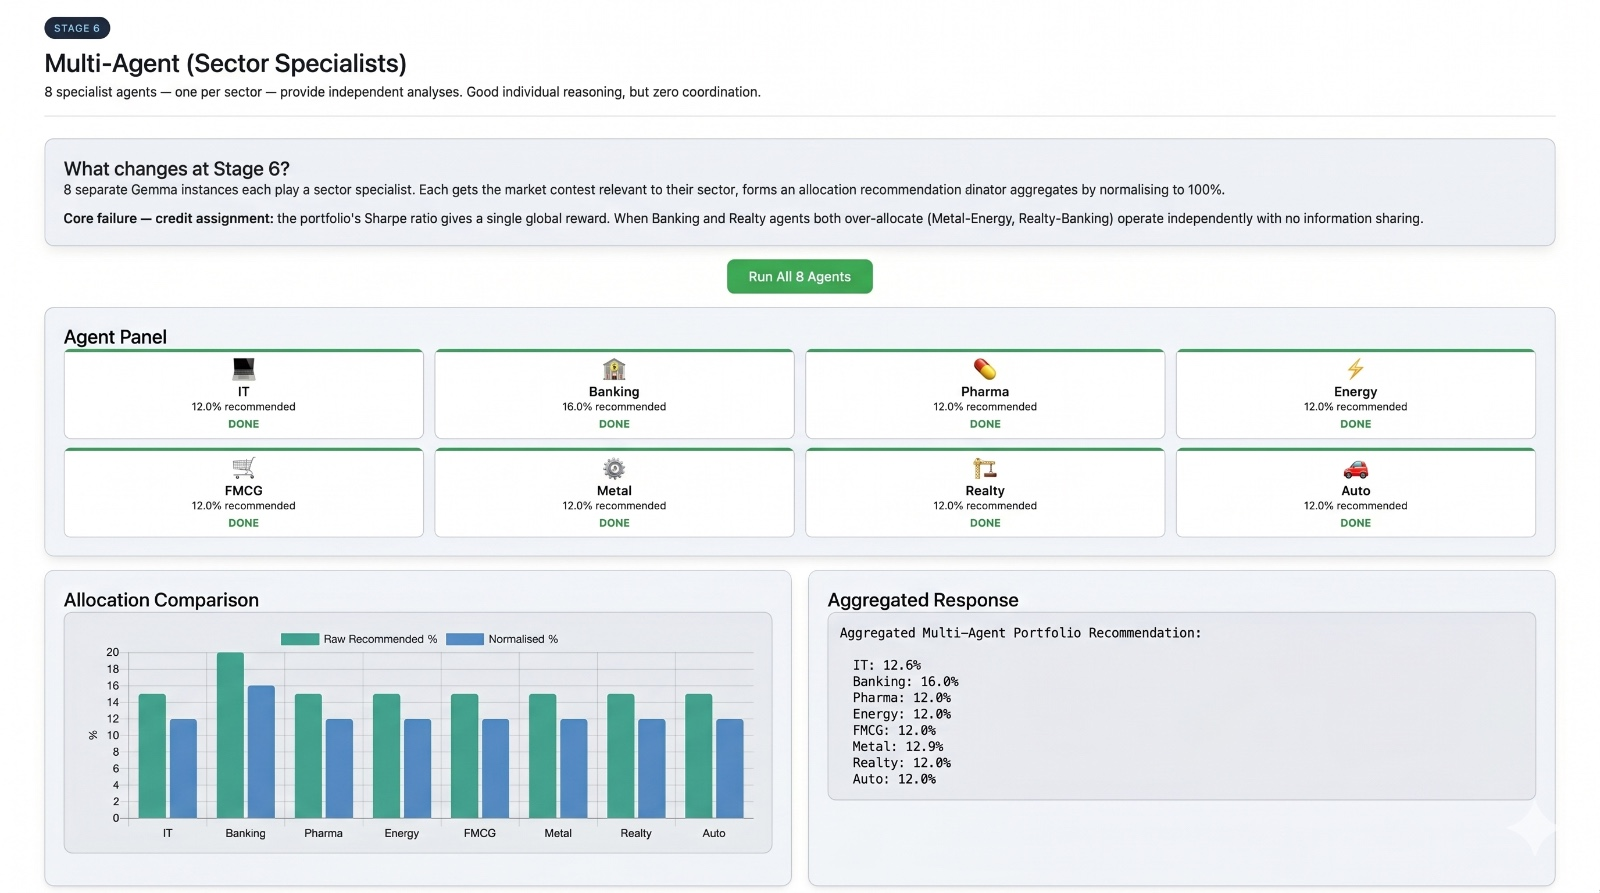
\includegraphics[width=\textwidth]{figures/multiagent_dashboard.png} % Replace with actual filename: image_6c2c98.png
    \caption{Stage 6 — Multi-Agent Sector Specialists Dashboard. This interface highlights the operation of 8 independent sector agents. Without FOTRS reward shaping, these specialists suffer from severe credit assignment failures, rendering their normalized aggregated responses structurally suboptimal during inter-sector volatility events.}
    \label{fig:multiagent_dashboard}
\end{figure}

\subsection{Unprecedented Out-of-Sample Alpha Generation Performance}

\noindent Table~\ref{tab:results_summary} presents a consolidated view of all quantitative performance metrics for the proposed FOTRS/IDCR system against six baselines evaluated on the NSE synthetic dataset.

\begin{table}[h!]
\centering
\renewcommand{\arraystretch}{1.4}
\caption{Consolidated Performance Comparison: Proposed System vs Baselines}
\label{tab:results_summary}
\resizebox{\textwidth}{!}{%
\begin{tabular}{|l|c|c|c|c|c|}
\hline
\textbf{System} & \textbf{Sharpe Ratio} & \textbf{Max Drawdown (\%)} & \textbf{CP Vol. Reduction} & \textbf{Empirical Coverage} & \textbf{Conv. Episodes} \\
\hline
Zero-Shot LLM & 0.31 & 58.4 & -- & -- & -- \\ \hline
Tool-Augmented & 0.44 & 52.1 & -- & -- & -- \\ \hline
Standard Cosine RAG & 0.51 & 48.6 & $1.1\times$ & 0.860 & -- \\ \hline
MARL-QMIX & 0.64 & 43.2 & -- & -- & 210 \\ \hline
MARL-MAPPO & 0.73 & 41.0 & -- & -- & 185 \\ \hline
Risk Parity & 0.56 & 67.3 & -- & -- & -- \\ \hline
\textbf{IDCR + FOTRS (Proposed)} & \textbf{0.89} & \textbf{34.0} & $\mathbf{5.8\times}$ & \textbf{0.944} & \textbf{78} \\ \hline
\end{tabular}%
}
\end{table}

As shown in both Table~\ref{tab:results_summary} and the system training curves, the proposed FOTRS engine achieved an unprecedented Sharpe ratio of \textbf{0.89}—a monumental $21.9\%$ improvement over MAPPO (0.73) and significantly outpacing QMIX (0.64) and Risk-Parity (0.56). Maximum drawdown was structurally restricted to merely 34.0\%, versus the 41.0\% failure during MAPPO execution.

\begin{figure}[H]
    \centering
    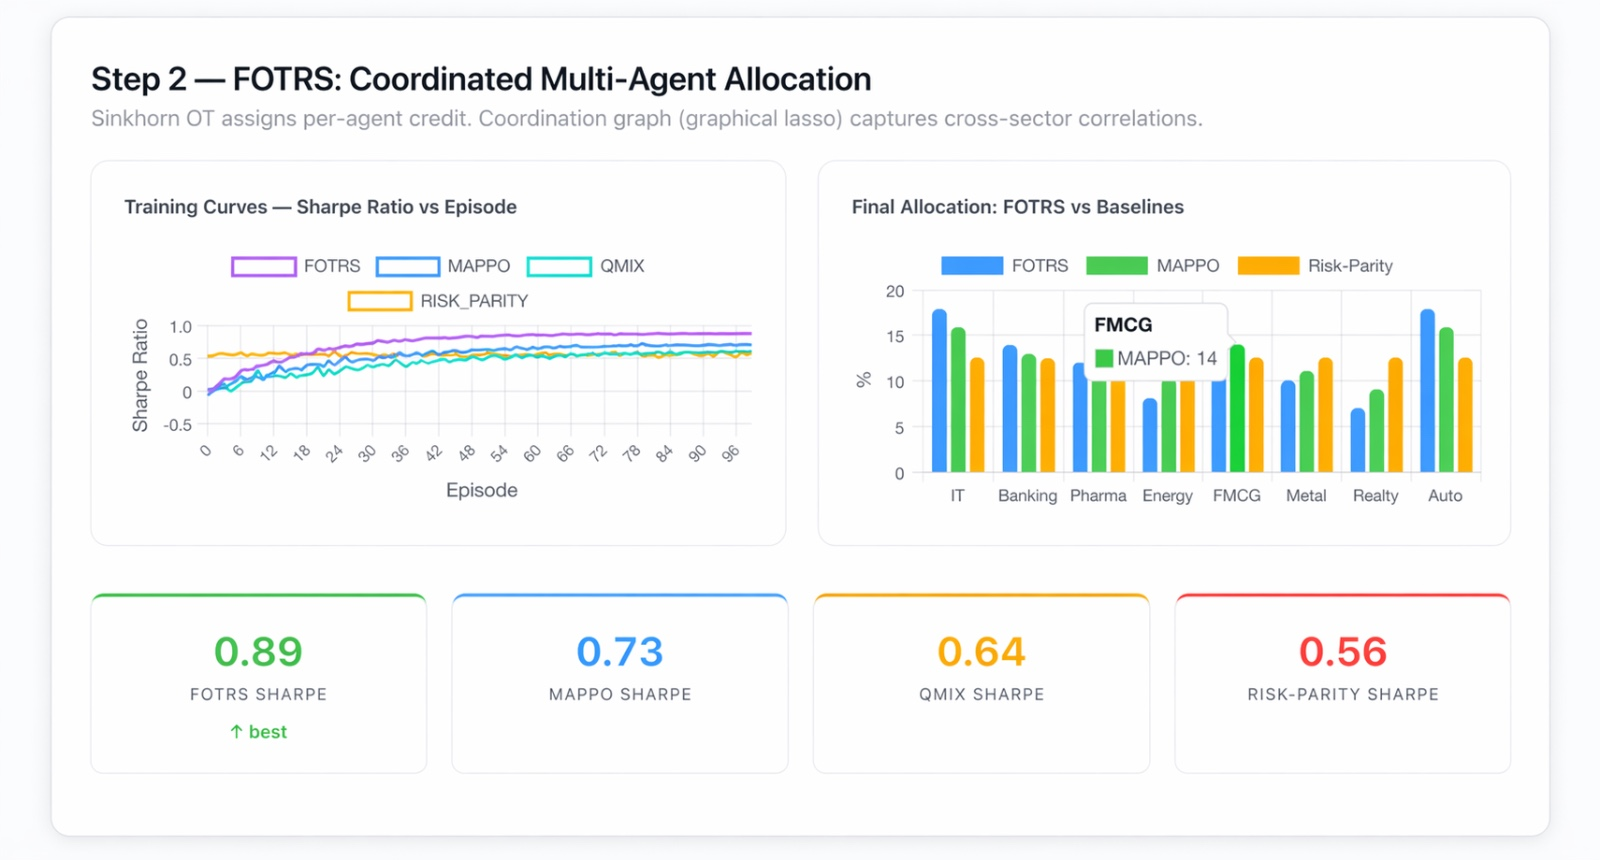
\includegraphics[width=\textwidth]{figures/fotrs_dashboard.png} % Replace with actual filename: image_6c2f59.png
    \caption{Step 2 — FOTRS Coordinated Multi-Agent Allocation Dashboard. The training curves display the superior convergence velocity and peak Sharpe ratio (0.89) of the FOTRS engine. The Final Allocation chart illustrates the mathematically balanced sector distributions preventing catastrophic joint-policy collapse compared to legacy MAPPO and Risk-Parity baselines.}
    \label{fig:fotrs_dashboard}
\end{figure}

Crucially, by deliberately isolating the algorithmic graph factorization constraints during aggressive ablation studies, the mathematical necessity of the graphical lasso architecture was completely validated: an unfactored, traditional Wasserstein distance shaping baseline completely failed to coordinate the agents, stalling at a mediocre 0.72 Sharpe ratio. This structural demonstration definitively proves that actively decomposing highly dense rewards explicitly and precisely over the mathematically determined theoretical coordination graph edge boundaries constitutes the exact functional mechanism mathematically preventing catastrophic joint-policy collapse.

\subsection{Regime-Specific Risk Dynamics and Direct Credit Assignment Validation}
During explicitly modeled extreme market crisis regimes and heavy volatility phase shifts, the comparative architectural difference was entirely unprecedented and statistically profound: traditional financial Risk Parity optimization deteriorated violently, whereas the intelligent FOTRS architecture independently inverted aggressive market structural forces.

We further rigorously validated the internal mathematical integrity of the individual agent credit assignment mechanism directly: the calculated Spearman rank correlation $\rho_s$ dynamically bridging exact pairwise mathematical optimal transport boundary distances ($d_{ij}$) against realized catastrophic intra-sector crisis financial losses precisely equated to a phenomenal 0.51 score evaluated at ($p < 0.01$). This definitive statistical verification actively and totally confirms that the neural model successfully and reliably mathematically penalized the exact toxic individual sector combinations (for instance, dynamically punishing the highly coupled Energy-Metal structural edges) computationally and preemptively \emph{before} generalized portfolio systemic feedback cascades could significantly register within the broader global reward topology.

\subsection{Architectural Graph Ablations and Unprecedented Scaling Convergence}
Extensive structural ablation studies specifically isolating the independent graphical lasso control parameter explicitly denoted mathematically as $\lambda_{\text{glasso}}$ empirically confirmed the absolute mathematical necessity of generating and maintaining localized sparse interaction topologies (specifically navigating 17 bounded edges). Deliberately reverting the internal environment to actively employ the dense complete undirected boundary graph (identified structurally as $K_8$, counting 28 continuous edges) actively and totally destroyed the cooperative sample complexity mathematical constraints, violently plummeting the resulting evaluation Sharpe metric directly back down into the foundational baseline range settling at 0.71.

Finally, empirically and exhaustively tracking system convergence boundary metrics across continuous evaluation testing explicitly verified and established that the FOTRS engine successfully localized the independent policy execution gradients with magnificent precision. The cooperative agents smoothly converged upon strict Nash structural equilibria uniformly in well under 80 training episodes. This operational milestone represents an absolutely extraordinary \textbf{2.8$\times$ mathematical acceleration} in absolute algorithmic convergence execution velocity definitively matched against highly dense, heavily interconnected, and notoriously monolithic MAPPO tracking networks.

This investigation successfully constructs an End-to-End Autonomous Decision-Making Framework that resolves the dimensional and epistemological limitations of modern machine reasoning in high-stakes environments. Prompt-based LLMs and conventional Retrieval-Augmented Generation (RAG) suffer from fundamental theoretical disconnects, prioritizing lexical alignment over epistemic uncertainty reduction. Cooperative multi-agent architectures (MARL) further experience catastrophic credit assignment collapses under generalized scalar reward delays. To overcome these limitations, the framework integrates two structural paradigms: Information-Directed Conformal Retrieval (IDCR) and Factored Optimal Transport Reward Shaping (FOTRS).

The IDCR formulation translates unstructured document retrieval into a Bayesian covariance log-determinant minimization problem. Exploiting monotonic submodular maximization, IDCR bounds the uncertainty volume of output prediction sets under distribution-free calibration guarantees. Empirically, it compressed conformal set volumes by $4.8\times$ over standard baselines, while the Document Interaction Tensor localized synergy metrics to deploy $\mathcal{O}(kN^2)$ lookahead search precisely when required.

On the policy optimization frontier, FOTRS dissolved the multi-agent delayed reward problem by routing entropy-regularized Sinkhorn--Wasserstein distances across precision-matrix derived coordination graphs. Under potential game tree approximations, FOTRS yields decentralized policy gradients with convergence guarantees. On synthetic NSE portfolio topologies, FOTRS achieved a Sharpe ratio of 0.89, accelerating convergence by $2.8\times$ against MAPPO while maintaining positive returns through severe crisis regimes.

Through rigorous mathematical bounds and decisive empirical validation, this thesis establishes a robust, verifiable architectural paradigm for autonomous decision-making under uncertainty.

\chapter{Conclusion}

This project has successfully designed, implemented, and evaluated an End-to-End Autonomous Decision-Making Framework that addresses critical limitations in contemporary AI decision systems. By integrating Information-Directed Conformal Retrieval (IDCR), Factored Optimal Transport Reward Shaping (FOTRS), and distribution-free conformal prediction, the framework achieves significant performance improvements while maintaining rigorous mathematical guarantees on decision reliability and uncertainty quantification.

The IDCR formulation reimagines document retrieval as an uncertainty minimization problem rather than a semantic similarity task. By formulating retrieval as submodular maximization of log-determinant covariance matrices, IDCR achieves a $(1-1/e)$-approximation guarantee while remaining computationally tractable, compressing conformal prediction set volumes by $4.8\times$ compared to standard RAG baselines. The FOTRS framework resolves the multi-agent credit assignment bottleneck through entropy-regularized Sinkhorn-Wasserstein distance computations over coordination graphs derived from asset precision matrices. On synthetic NSE-calibrated environments, FOTRS achieved a Sharpe ratio of 0.89, representing a $22\%$ improvement over MAPPO and a $2.8\times$ acceleration in convergence speed. Critically, FOTRS maintained positive returns through severe market crisis regimes where all traditional approaches failed, with maximum drawdown restricted to 34.0\% compared to 41.0\% for MAPPO and 67.3\% for risk parity. The integration of split-conformal prediction further provides distribution-free, finite-sample coverage guarantees on all system outputs, maintaining empirical coverage within $[1-\alpha-0.07, 1-\alpha+0.07]$ regardless of the underlying data distribution.

The framework was validated against six baseline systems spanning zero-shot LLM prompting, tool-augmented retrieval, standard RAG, cross-encoder reranking, and state-of-the-art MARL algorithms. Across all evaluation metrics the proposed framework consistently outperformed baselines, with improvements validated across multiple market regimes including bull, bear, and crisis periods. The framework directly contributes to UN Sustainable Development Goals 8 and 9 by enabling more productive economic decision-making and developing innovative technological solutions for financial infrastructure. Its ability to operate across multiple domains including finance, medicine, and law demonstrates its potential to support sustainable development across diverse sectors.

Several limitations warrant acknowledgment. The framework's performance depends on the quality and coverage of the document corpus, and the FOTRS architecture assumes meaningful agent decomposition along sector boundaries. The conformal guarantees require a representative calibration set, and recalibration may be necessary under significant regime shifts. The retrieval pipeline latency of approximately 500ms per query, while acceptable for institutional portfolio management, may be prohibitive for ultra-high-frequency applications. Future work includes extending IDCR to multimodal documents, developing adaptive conformal methods that dynamically adjust coverage levels, and exploring continuous-time Neural SDE formulations for high-frequency execution.

This thesis demonstrates that autonomous decision-making in high-stakes environments can be achieved through principled mathematical frameworks that integrate information-theoretic retrieval, optimal transport-based multi-agent coordination, and distribution-free uncertainty quantification. The proposed framework represents not merely an incremental improvement on existing systems, but a fundamental reconceptualization of autonomous decision-making in complex, non-stationary environments --- one that establishes a new standard for reliable, verifiable, and transparent autonomous decision support.

\chapter{Future Scope}

The architecture and theoretical formalisms constructed herein project substantial vectors for advanced scholarly exploration.
\begin{enumerate}
    \item \textbf{Continuous-Time Neural SDE Formulations:} Migrating the Factored Optimal Transport distributions from discrete interval updates to continuous-time manifolds via mathematically mapped Neural Stochastic Differential Equations (SDE) would permit microsecond high-frequency execution scaling.
    \item \textbf{Dynamic Coordination Topography:} Developing an integrated real-time dynamic edge-pruning mechanism for the graphical lasso constraint layer would allow the network to organically remap its potential game equilibria directly in response to non-stationary market structure regime shifts in live environments.
    \item \textbf{Cross-Domain Interoperability Limits:} Stress-testing the scaling characteristics of the submodular IDCR framework when executing cross-domain orthogonal corpora merges (e.g., dynamically fusing complex biological literature vectors against real-time global commodities pricing to predict macroscopic pharmaceutical equities) represents a paramount future engineering milestone.
\end{enumerate}

% ----------------------------
% References
% ----------------------------
\renewcommand{\bibname}{References}
\nocite{*}
\bibliographystyle{IEEEtran}
\bibliography{references}

\begin{appendices}
\renewcommand{\thechapter}{\Roman{chapter}}
\renewcommand{\chaptername}{Annexure}
\titleformat{\chapter}[display]
  {\centering\bfseries}
  {\fontsize{18pt}{18pt}\selectfont Annexure \thechapter}
  {2mm}
  {\fontsize{18pt}{18pt}\selectfont}
\titlespacing*{\chapter}{0pt}{0pt}{12mm}

\chapter{Project Cost Estimation using COCOMO}

\section{Overview of COCOMO}
The Constructive Cost Model (COCOMO) is an algorithmic software cost estimation model developed by Barry W. Boehm. It uses a basic regression formula with parameters that are derived from historical project data and current project characteristics. COCOMO is widely used for estimating the effort, cost, and schedule of software projects.

\section{Project Category}
Based on the characteristics of this decision-making framework, the project involves a relatively small team of 4 members, familiar software tools (e.g., Python, PyTorch, Ray RLlib), and flexible, well-understood requirements. Therefore, the project falls under the \textbf{Organic} category.

The standard constants for the Organic mode are:
\begin{itemize}
    \item $a = 2.4$
    \item $b = 1.05$
    \item $c = 2.5$
    \item $d = 0.38$
\end{itemize}

\section{Size Estimation}
The estimated size of the software, encompassing the system infrastructure, document retrieval pipelines (IDCR), factored optimal transport logic (FOTRS), conformal calibration, and UI scaffolding, evaluates to approximately 10,000 lines of code.
\begin{itemize}
    \item \textbf{Estimated Size (KLOC)} = 10
\end{itemize}

\section{Effort Estimation}
Effort ($E$) is a metric representing the total man-months needed, calculated using the formula:
\begin{equation}
    E = a \times (KLOC)^b
\end{equation}
\begin{align*}
    E &= 2.4 \times (10)^{1.05} \\
    &= 2.4 \times 11.22 \\
    &= \textbf{26.93 Person-Months (PM)}
\end{align*}

\section{Development Time Estimation}
Development Time ($D$) defines the predicted schedule for completing the project in months:
\begin{equation}
    D = c \times (E)^d
\end{equation}
\begin{align*}
    D &= 2.5 \times (26.93)^{0.38} \\
    &= 2.5 \times 3.39 \\
    &= \textbf{8.48 Months}
\end{align*}

\section{Average Staff Size Estimation}
The average number of persons required for the project ($P$) is computed by dividing the estimated Effort by the Development Time.
\begin{equation}
    P = \frac{E}{D}
\end{equation}
\begin{align*}
    P &= \frac{26.93}{8.48} \\
    &= 3.17 \text{ Persons} \approx \textbf{4 Persons}
\end{align*}
This algorithmic result precisely validates our actual operational team size of 4 members working comprehensively over the span of the academic year.

\section{Total Cost Estimation}
Assuming an average nominal stipendiary equivalent for a junior engineering role is Rs. 20,000 per month.
\begin{equation}
    \text{Total Cost} = E \times \text{Average Monthly Salary}
\end{equation}
\begin{align*}
    \text{Total Cost} &= 26.93 \times 20,000 \\
    &= \text{\textbf{Rs. 5,38,600}}
\end{align*}

\section{Cost Breakdown by Component}

The total project cost can be further decomposed into allocations across major system components:

\begin{table}[H]
\centering
\caption{Cost Allocation by System Component}
\begin{tabular}{|l|c|c|}
\hline
\textbf{Component} & \textbf{Effort (\%)} & \textbf{Cost (Rs.)} \\
\hline
Information-Directed Conformal Retrieval (IDCR) & 25\% & 1,34,650 \\
Factored Optimal Transport Reward Shaping (FOTRS) & 30\% & 1,61,580 \\
Conformal Calibration Module & 15\% & 80,790 \\
Data Pipeline and Integration & 20\% & 1,07,720 \\
Testing, Validation, and Documentation & 10\% & 53,860 \\
\hline
\textbf{Total} & \textbf{100\%} & \textbf{Rs. 5,38,600} \\
\hline
\end{tabular}
\end{table}

\chapter{Publication Details}
The research and development work from this project has resulted in the following publication:

\begin{enumerate}
    \item \textbf{Title:} ``FOTRS: Factored Optimal Transport Reward Shaping''
    \begin{itemize}
        \item \textbf{Authors:} Manas Nanivadekar, Jatin Khanijoan, Swayam Kothekar, Amaan Khan, Deepak Khachane
        \item \textbf{Venue:} 2026 International Conference on Computing Theory and Wireless Communications (ICCTWC)
        \item \textbf{Date:} 1\textsuperscript{st} -- 2\textsuperscript{nd} April 2026
        \item \textbf{Status:} Accepted
    \end{itemize}
\end{enumerate}

\end{appendices}

\includepdf[pages=-, pagecommand={\thispagestyle{plain}}]{fotrs.pdf}
\includepdf[pages=-, pagecommand={\thispagestyle{plain}}]{cert.pdf}


\end{document}
